In this chapter, we present applications of the anomaly detection models described in Chapter \ref{chapter:models-and-algorithms-for-anomaly-detection}.
%We start our experiments by applying probabilistic models.
In the beginning, we apply GMM, which does not take into account the sequential feature of the data, and then we implement the HMM, which is a probabilistic sequence model.
Then, we expand our work with the application of deep learning sequence models. 
We perform experiments and compare the results with models constructed on RNN and LSTM, respectively.

In the experiments, we will use the Borusan wind turbine dataset.
%and NASA Aircraft Engine datasets \cite{saxena2008damage, bao2018remaining}.

\section{Wind Turbine Dataset}

%We used Borusan Vestas V90-3MW wind turbines dataset as the first application of anomaly detection problem.
Borusan Vestas V90-3MW wind turbines dataset was created from 20 different wind turbines which are identical.
For each wind turbine, there are observations collected at 25737 different consecutive time-steps.
Each observation is the collection of wind speed, rotor speed, and generated power values.
This data set was created with data collected at 10-minute intervals from February to July.
There are only two reported anomalies in the data set. 
However, it is known that there are unreported and undetected anomalies.
Additionally, this dataset contains some Null and incorrect sensory information because of the faulty sensor measurements.
These errors occur randomly and do not continue.
Therefore, we know that there is no accurate data in the data set and that there are errors and missing data in the observations. The visualization of the wind, rotor, and power data could be found in Figure \ref{fig:data}.

\begin{figure}
\centering
    \subfigure[Wind speed graph as a time-series]{
        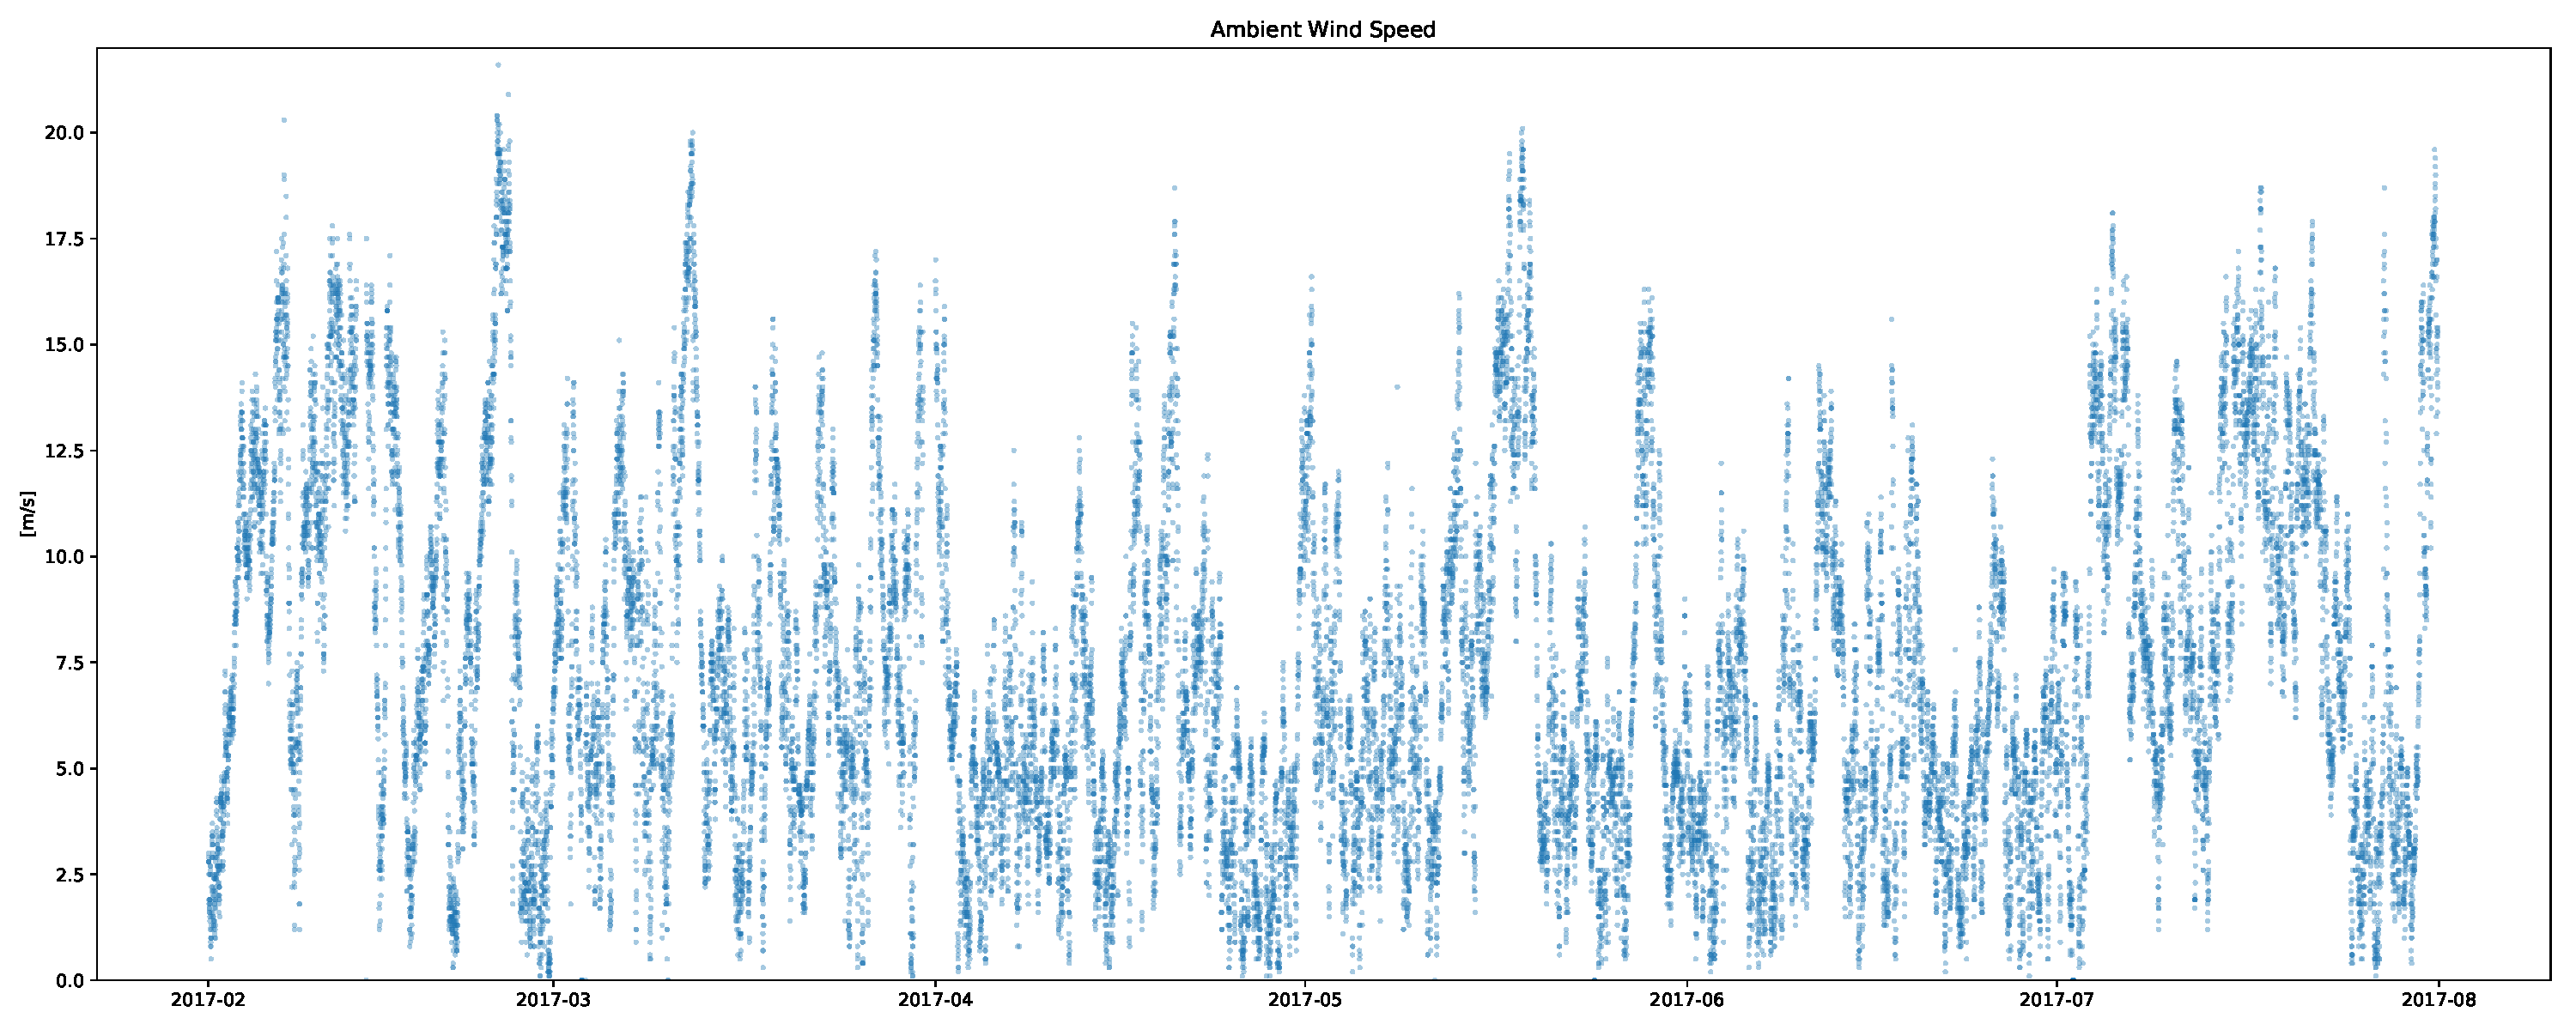
\includegraphics[width=0.9\textwidth]{wind.pdf}
        \label{fig:wind}
    }%
    
    \subfigure[Rotor speed graph as a time-series]{
        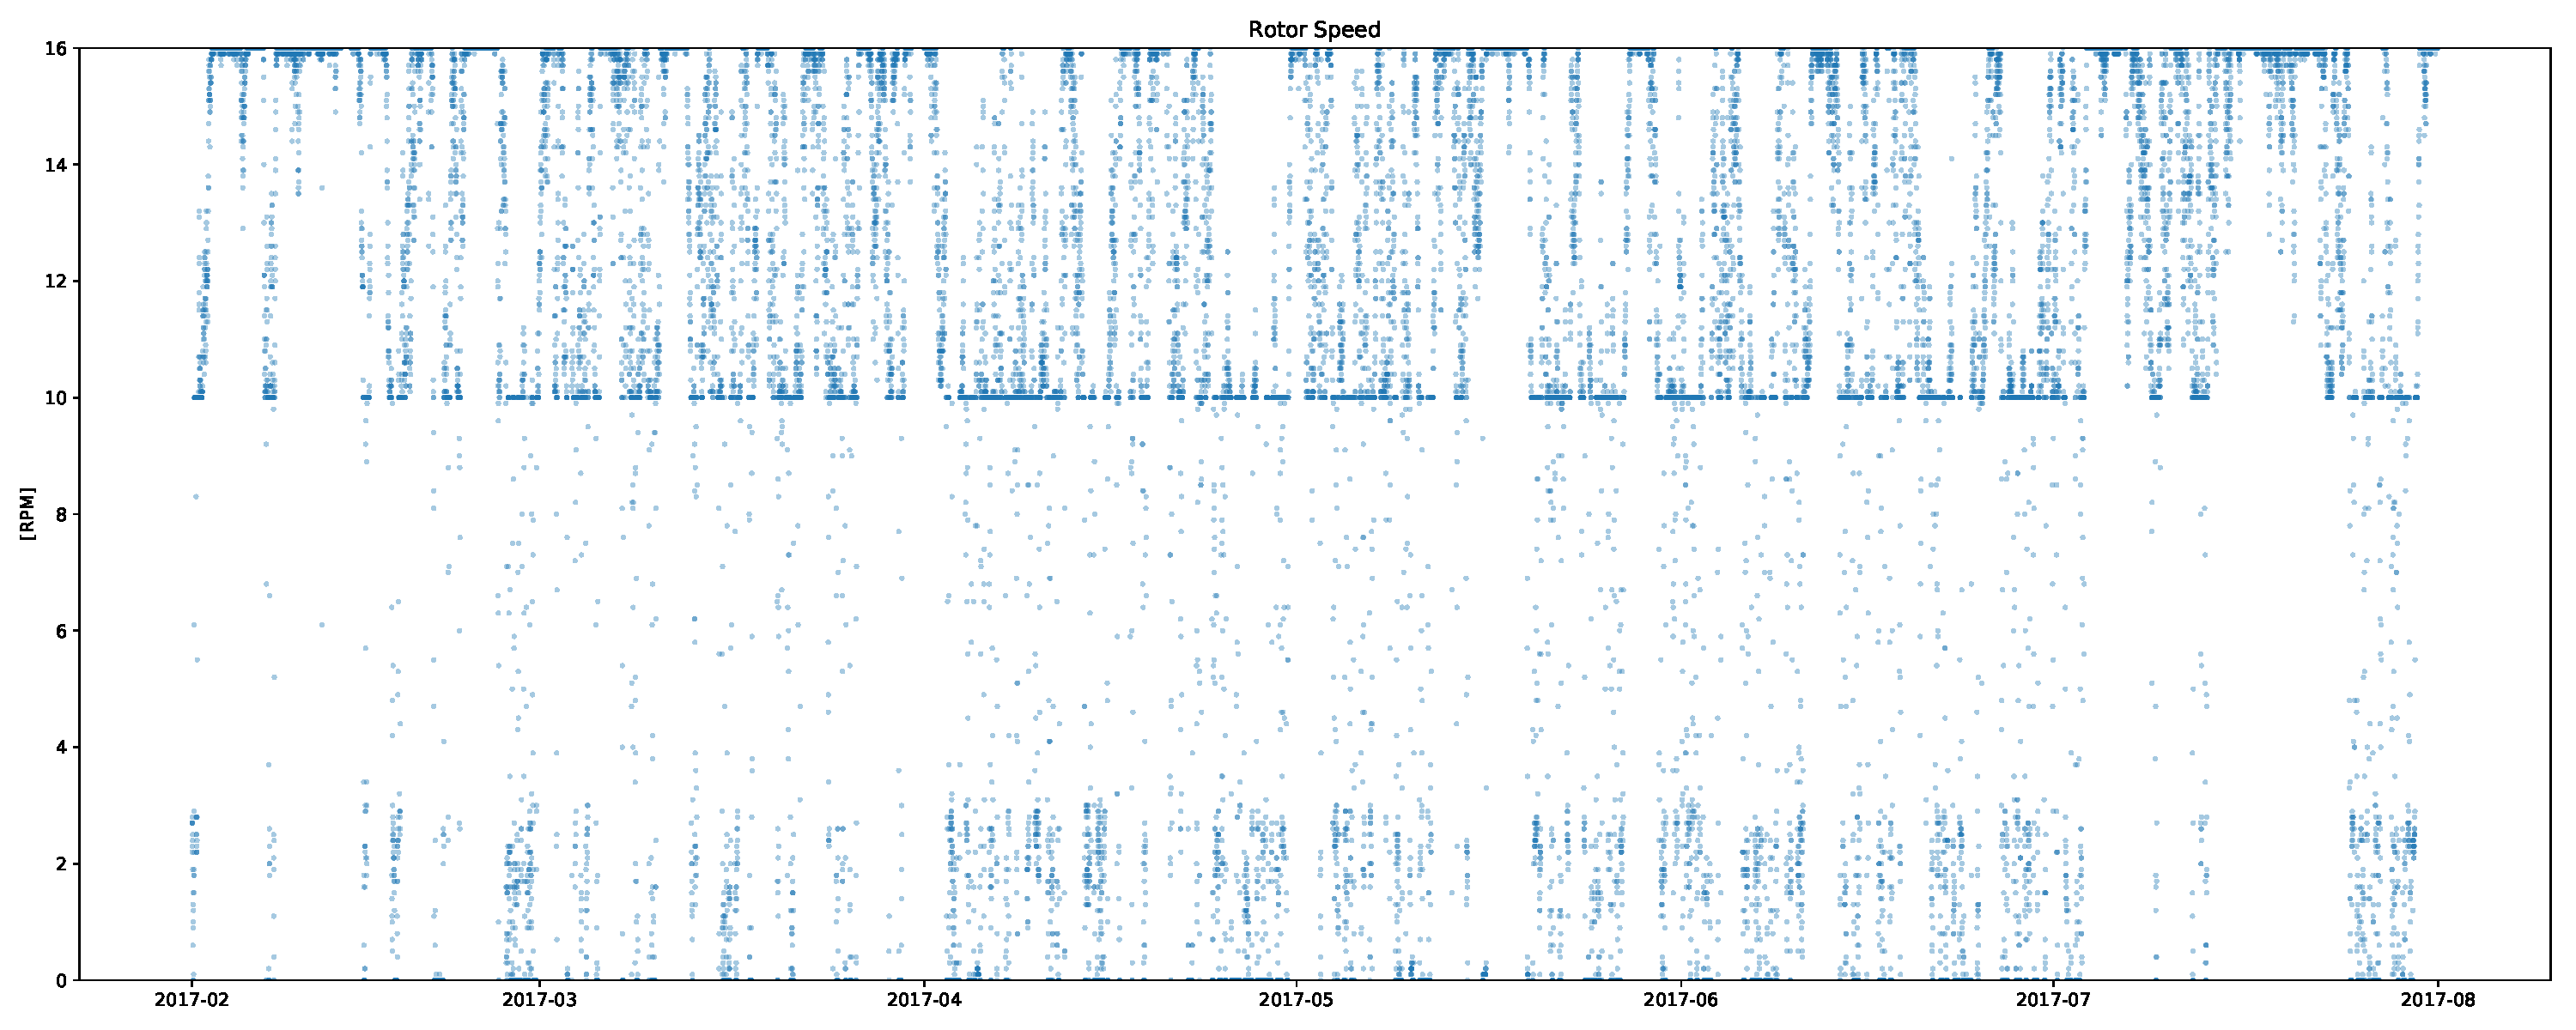
\includegraphics[width=0.9\textwidth]{rotor.pdf}
        \label{fig:rotor}
    }%
    
    \subfigure[Generated grid power graph as a time series]{
        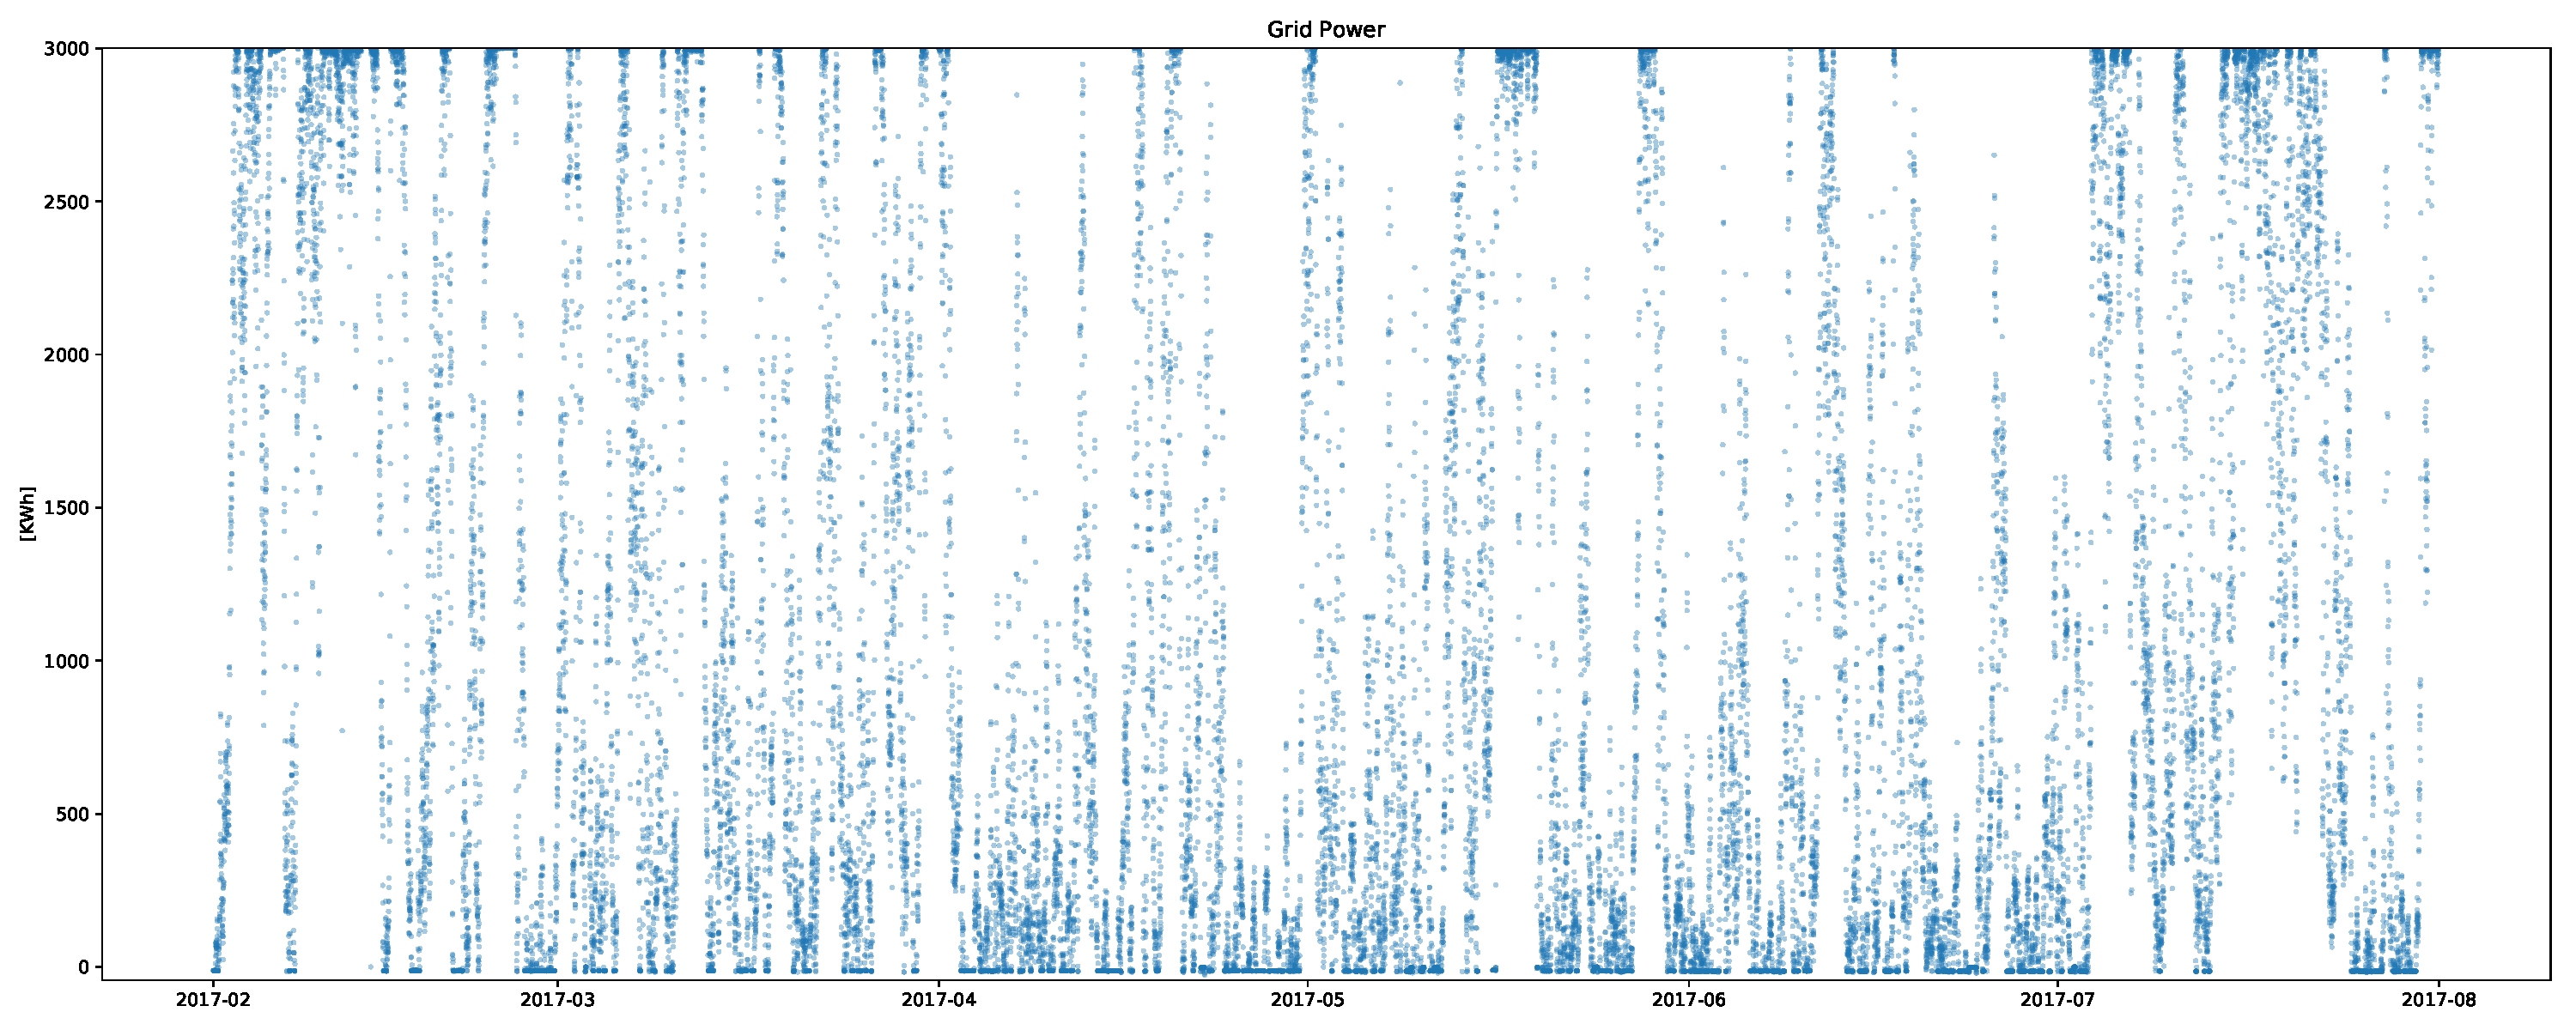
\includegraphics[width=0.9\textwidth]{grid_power.pdf}
        \label{fig:grid_power}
    }
    \caption{Individual sequential graphs for the sensory information}
    \label{fig:data}
\end{figure}

In this dataset, wind speed can be seen as an input to the system while the rotor speed and the generated power are the outputs of the system. However, it can be seen from Figure~\ref{fig:data} that there is not a direct relationship between these features. The reason behind this phenomena is that previous observations and working condition of the turbine affect the current time observations because of the physical relationships in the mechanical system of the wind turbines. Therefore, the outputs cannot be generated directly according to input data, and it requires the system state, which indicates how the system reacts to the given input. 
The interaction graph which is obtained from a limited time interval and does not consider the time series feature can be seen in Figure~\ref{fig:powercurve}.

\begin{figure}
    \centering
    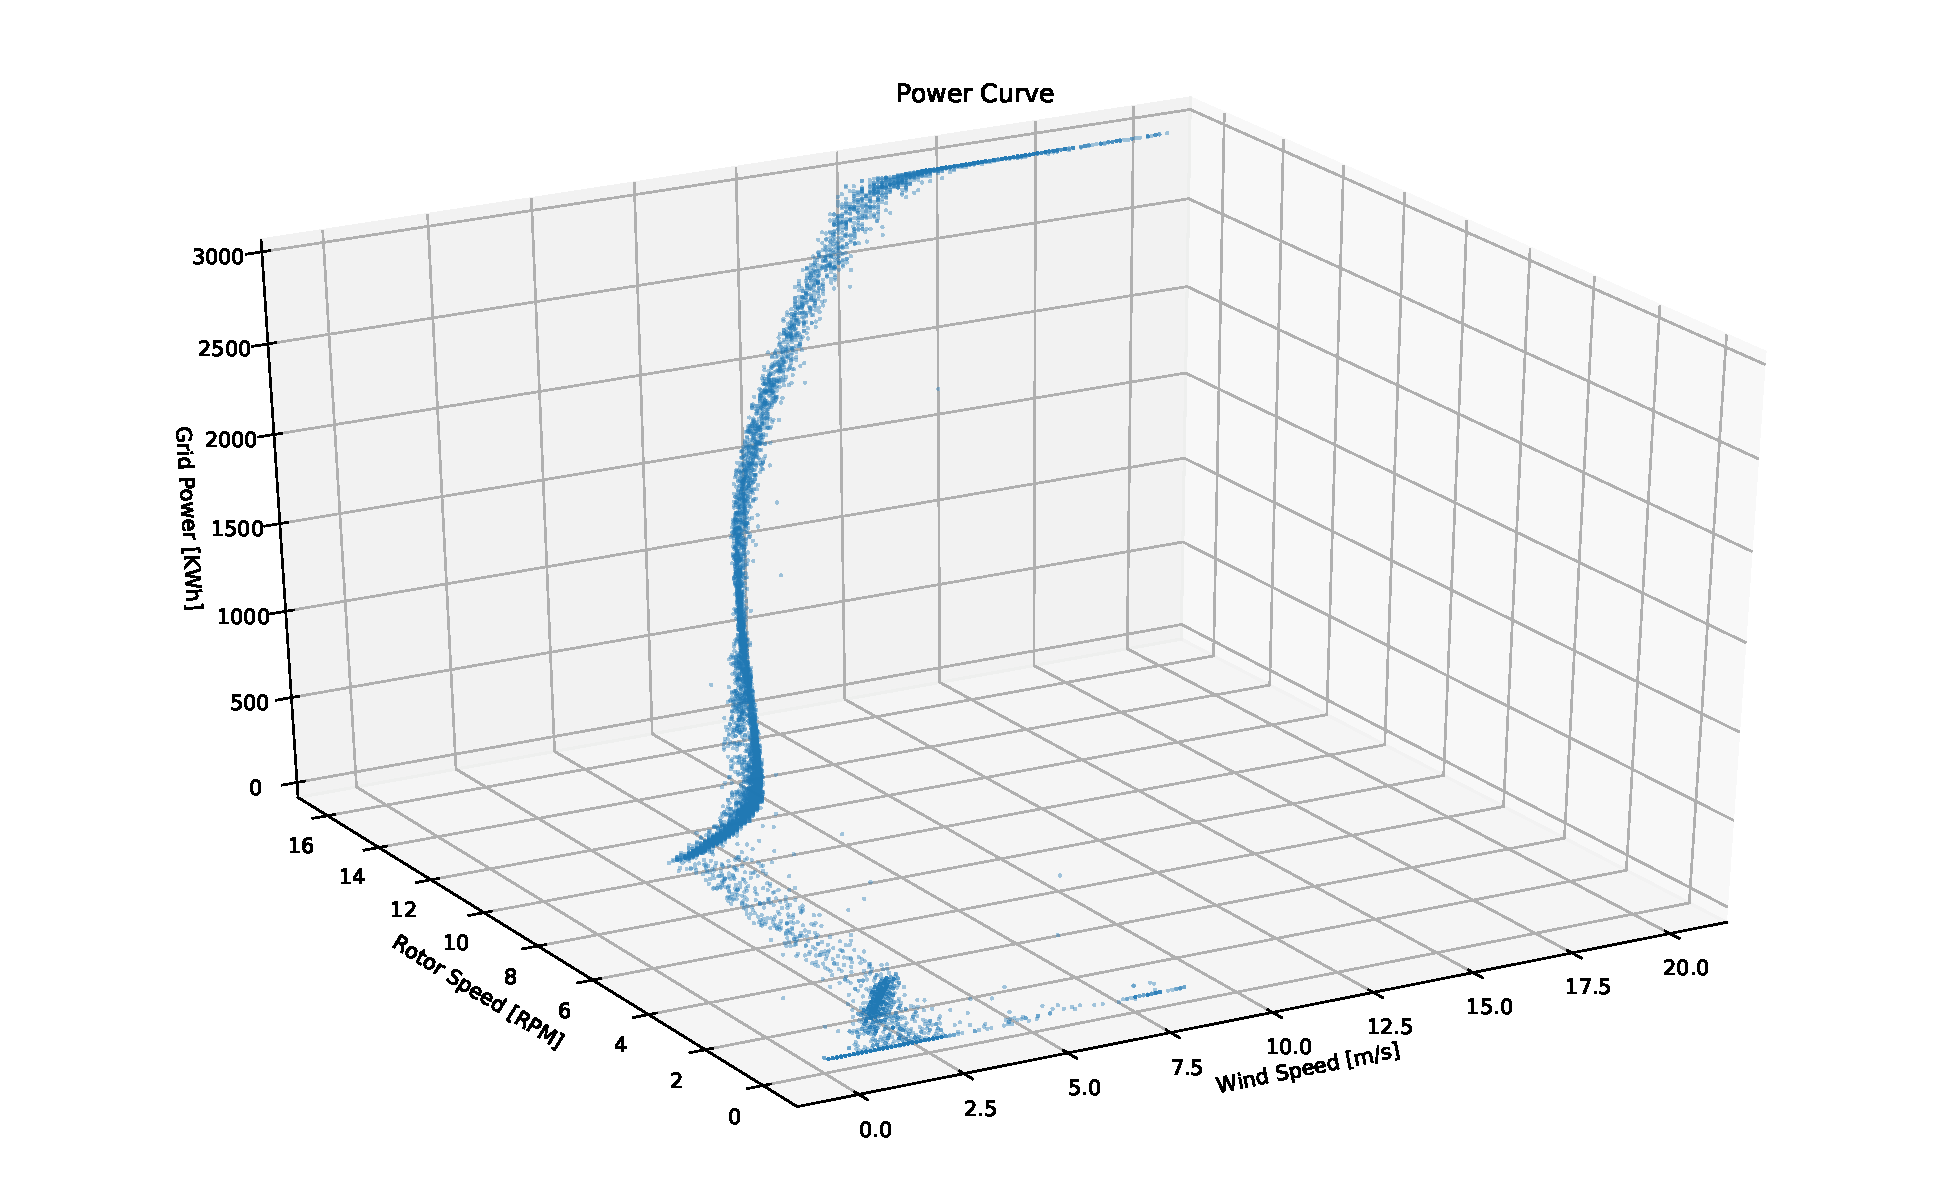
\includegraphics[width=\textwidth]{power.pdf}
    \caption{The relationship between the wind speed, rotor speed and grid power}
    \label{fig:powercurve}
\end{figure}

\subsection{Modeling The Power Curve of Wind Turbine}

The power curve of wind turbines defines the relationship of a wind speed or rotor speed, or both, to the amount of power generation. Since, the physical machinery has a sophisticated control mechanism, as well as environmental variations that are not directly measurable, makes this relationship more complicated. Therefore, we have to create a model that works under different circumstances according to basic working principals of the wind turbines. For this purpose, we use Bayesian approaches to generate the power curve of the wind turbine efficiently.

There are different approaches to the modeling of the power curve. Some of the works use wind speed and grid power to evaluate the power curve \cite{ouyang:17} and some other uses rotor speed and grid power to evaluate power curve \cite{romero:16}. On the other hand, we use both rotor speed and wind speed because only wind cannot give too much information because it has too much uncertainty and there is a lot of sudden changes in the wind speed. On the other hand, rotor speed itself again cannot give desired results because there is break points in the rotor speed - power curve graph. In addition to that, such a discontinuity is not desired in such a model. Therefore we use both wind speed and rotor speed to analyze power curve model. By this selection, we see that the discontinuity in the rotor speed - grid power model is gone, and the high variance in the wind speed - power curve is also reduced. Therefore increasing the dimensionality of the power curve significantly strengthens our hands in terms of better analysis.

The power curve shows us the critical features of the wind turbine machinery system. However, although the wind speed, rotor speed, and grid power are included, the turbine still contains some discontinuity in the power curve as a result of some states of the turbine. Since there is a gearbox in the turbine, we expect that kind of relationship, and we can see the location of this change points from the power curve.

In addition to the previous details, we can also add the time factor to the account. When we do this, we create the power curve using the incoming data sequence. On this page, we can analyze not only the power curve but also the trends of change on the power curve.

We aim to find the optimum power curve for each turbine individually because the physical machines are complex systems, and even if they work with precisely the same mechanism, they can show different production values. The power curve includes the main line that the turbine is likely to generate and the variance that occurs. It is important to note that since wind turbines are rotating systems, the variance of the production will increase with the rotor speed. Therefore our model should take into account that property.

\subsection{Experiments with the Probabilistic Models}

We started this study by reconstruction of the power curves of the wind turbines using \textit {Gaussian Mixture Model}(GMM).
This model learns the power curve of the wind turbine as a mixture of Gaussian distribution over the available data. 
At this point, we assume that our observations include both turbine states and anomalies.
Therefore we assume that, in the model, there are $10$ different Gaussian distributions for turbine operation states which should be learned and there is $1$ Gaussian distribution with the infinite variance, uniform over output space, for sensory information errors or anomalies. 
These Gaussian distributions are then learned using the EM algorithm, except the distribution corresponds to anomalies.
Once the distributions are learned, we can determine which distribution the incoming data belongs to, and what observations are anomalies.
Therefore, according to this model, the incoming data has a predictive error rate. 
This model, which is more straightforward than HMM, does not take into account the time effect and how the consecutive observations should behave is not taken into account.
Therefore, the Gaussian distributions in the model are learned without this knowledge.
Since the incoming data is not analyzed as a time series, the model is more susceptible to faulty data coming from the sensors and can not catch the faulty transitions between states. The mixtures are shown in Figure~\ref{fig:gmm-mixtures}. Moreover, the model may be insufficient to detect unexpected fluctuations in the power output of the turbine.

\begin{figure}
\centering
    \subfigure[The mixture of Gaussians]{
        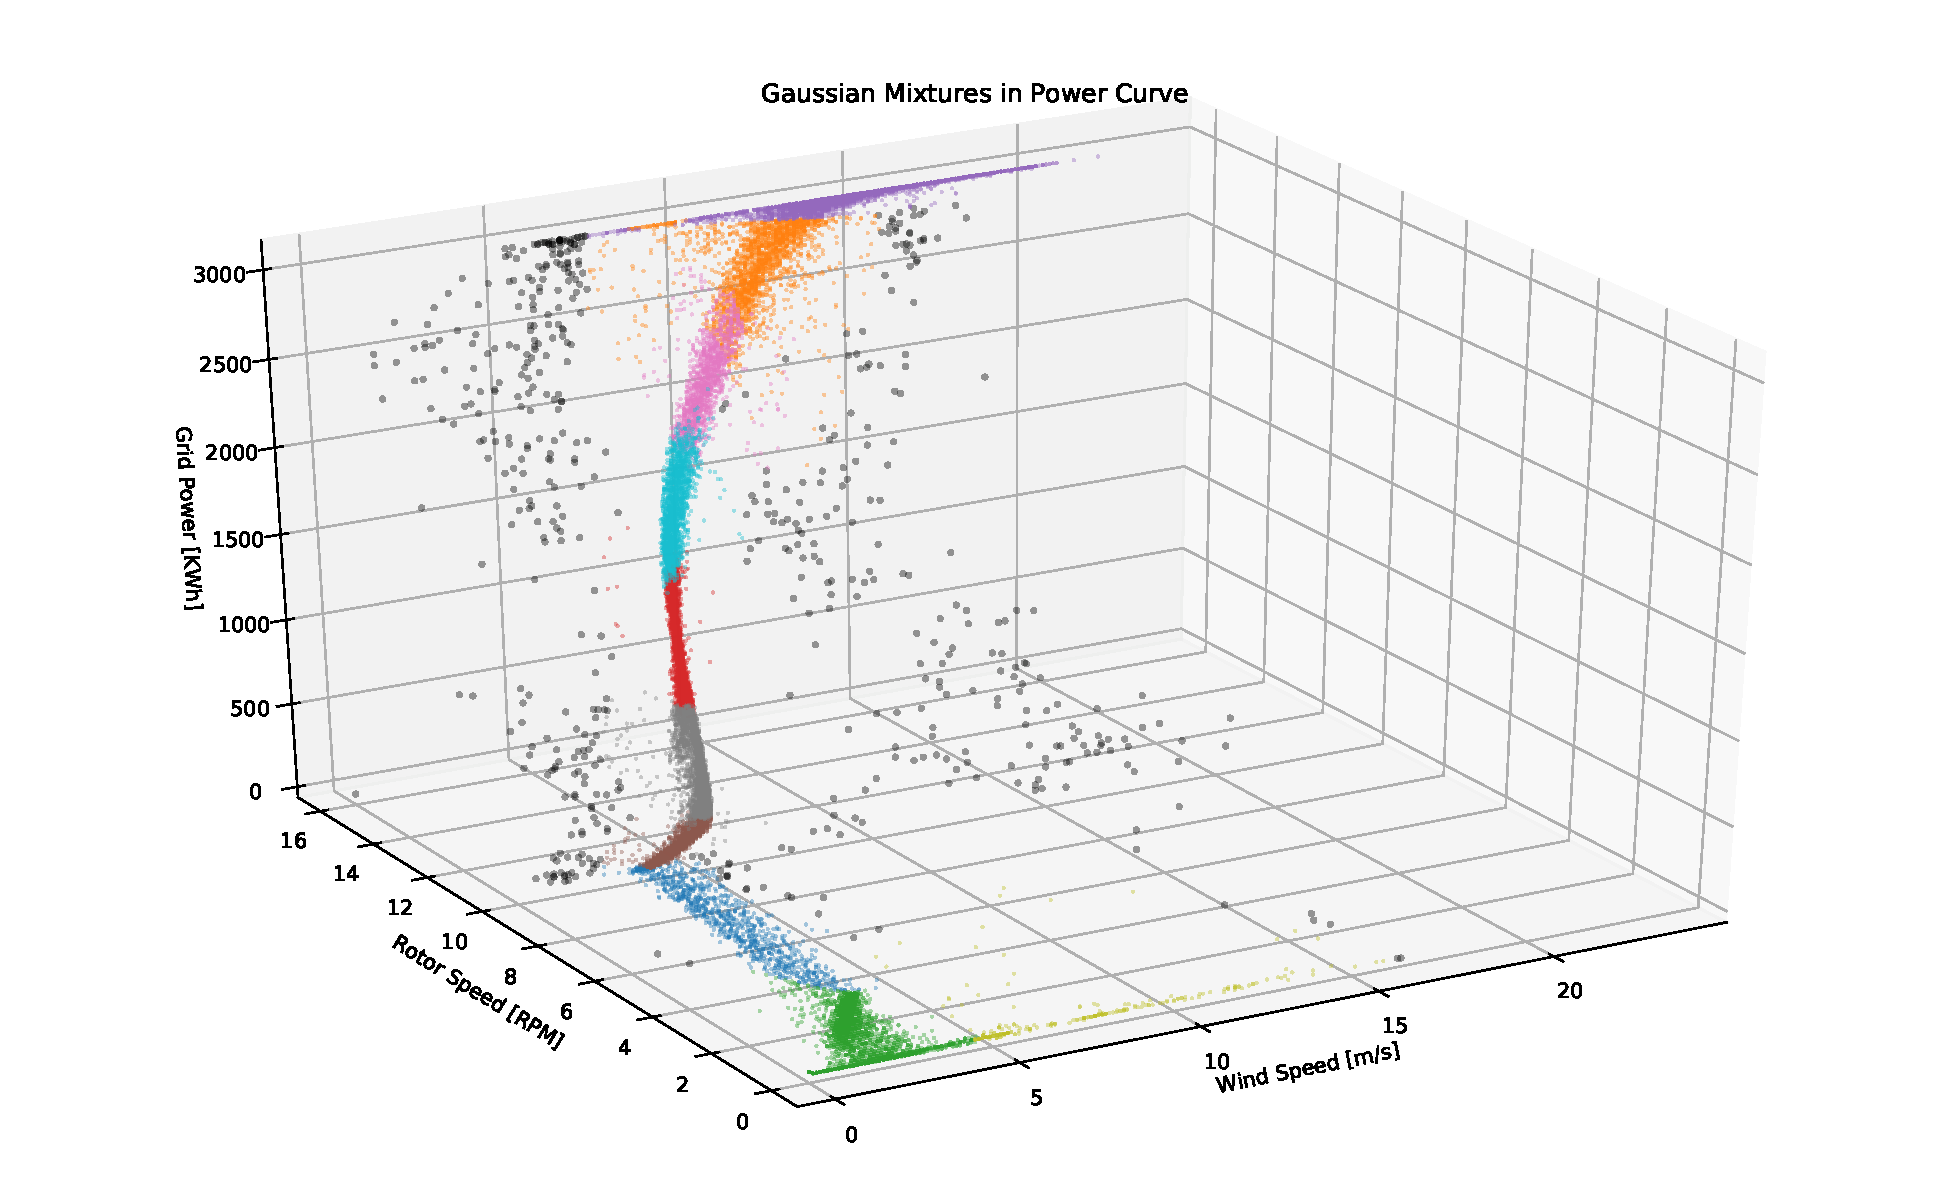
\includegraphics[width=0.95\textwidth]{gmm-mixtures.pdf}
        \label{fig:gmm-mixtures}
    }%
    
    \subfigure[Distributions in the latent space]{
        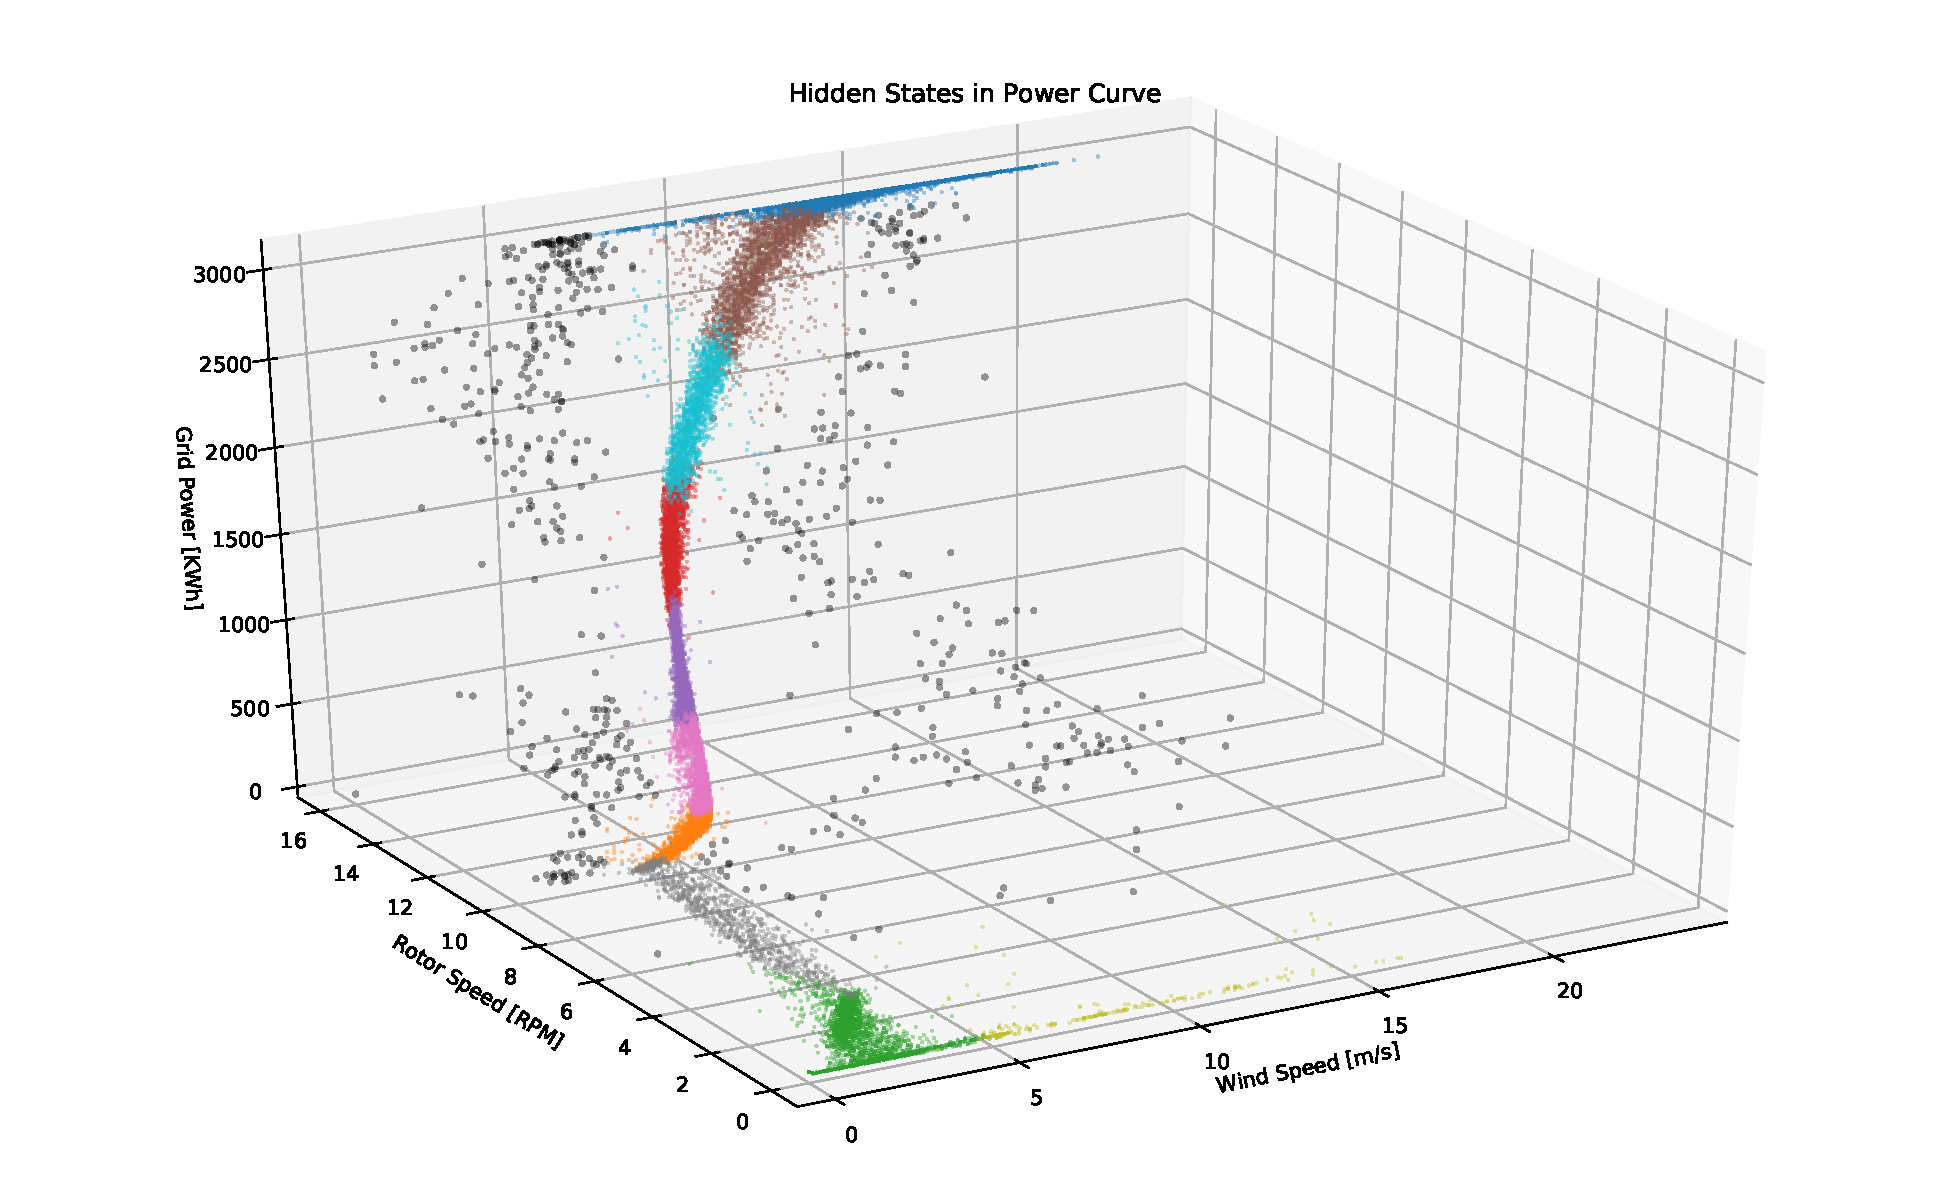
\includegraphics[width=0.95\textwidth]{hmm-mixtures.pdf}
        \label{fig:hmm-mixtures}
    }

    \caption{Comparison of the mixture of Gaussians in the GMM with distributions in the latent space of the HMM on the power curve.}
    \label{fig:mixtures}
\end{figure}

In the expanse of this study, the power curves of the wind turbines are constructed as time series using HMM. 
This model also learns the power curve of the wind turbine as a mixture of Gaussian distribution over the available data. 
Therefore we assume that, as in GMM, there are $10$ different Gaussian distributions for turbine operation states which should be learned and there is $1$ Gaussian distribution with the infinite variance, uniform over output space, for sensory information errors or anomalies. 
We design our model in such a way as to determine which distribution will come from which distribution.
Therefore, the previous distribution will have an impact on the distribution of the observations. Therefore the learned mixtures of the Gaussian distributions of the states will be slightly different from that obtained in the GMM.
The learned Gaussian mixtures by HMM are shown in Figure~\ref{fig:hmm-mixtures}. 
The better modeling of the system, as can be seen in Figure~\ref{fig:mixtures} has resulted in more obvious mixtures.
This model was trained by processing the sample mini-series of $144$ measurements, which corresponds to one-day observations. 
During this training, the learning speed was chosen as $\eta_t=1/\left(t+1\right)$. 
On the other hand, the state transition diagram of the HMM is shown in Figure~\ref{fig:transition}.
As can be seen from the transition diagram, it is possible to switch from any state to anomaly.
Therefore, the HMM model is more tolerant to incorrect measurements from the detectors and can detect abnormal changes in the power curve without being affected by false observations as it learns the operation of the turbine.
As a result of these studies, it can be seen that HMM can make error prediction more clear than GMM, according to Figure~\ref{fig:hmm-figc} and Figure~\ref{fig:hmm-figd}. However, the most critical point of HMM is that it minimizes the false positive error prediction. In most cases, the GMM tends to produce false positive predictions, as shown in Figure~\ref{fig:hmm-figf}, but HMM has achieved much better results in this regard. A detailed comparison between GMM and HMM model is given in Figure~\ref{fig:hmm-results}. Malfunctions are shown as black vertical lines in graphs. The collective anomaly result is cumulatively calculated from the anomaly forecast for each observation and converted into a warning signal.

\begin{figure}
    \centering
    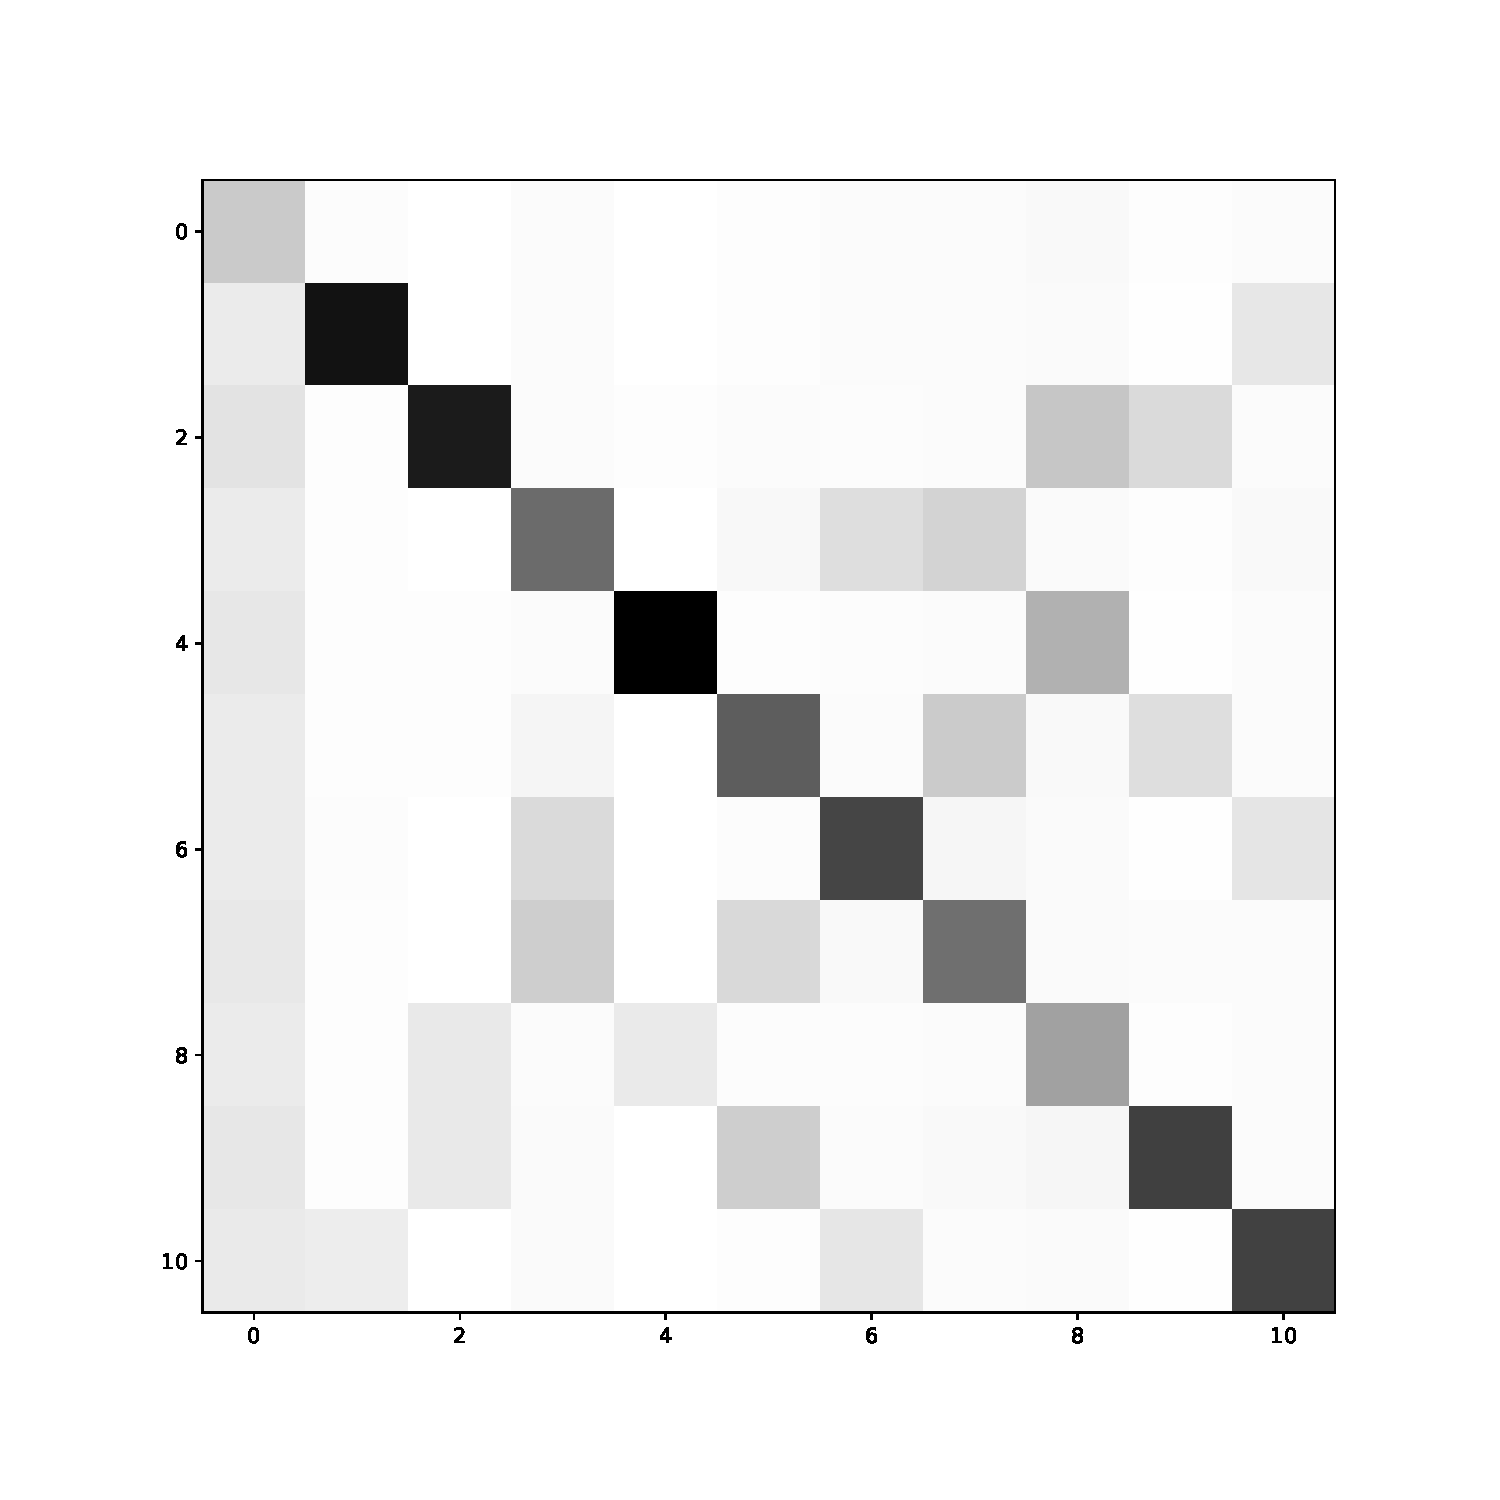
\includegraphics[width=0.6\textwidth]{transition.pdf}
    \caption{State transition diagram of the HMM}
    \label{fig:transition}
\end{figure}

\begin{figure}
    \centering
  \subfigure[The error prediction of HMM on the turbine which works under normal conditions]{
       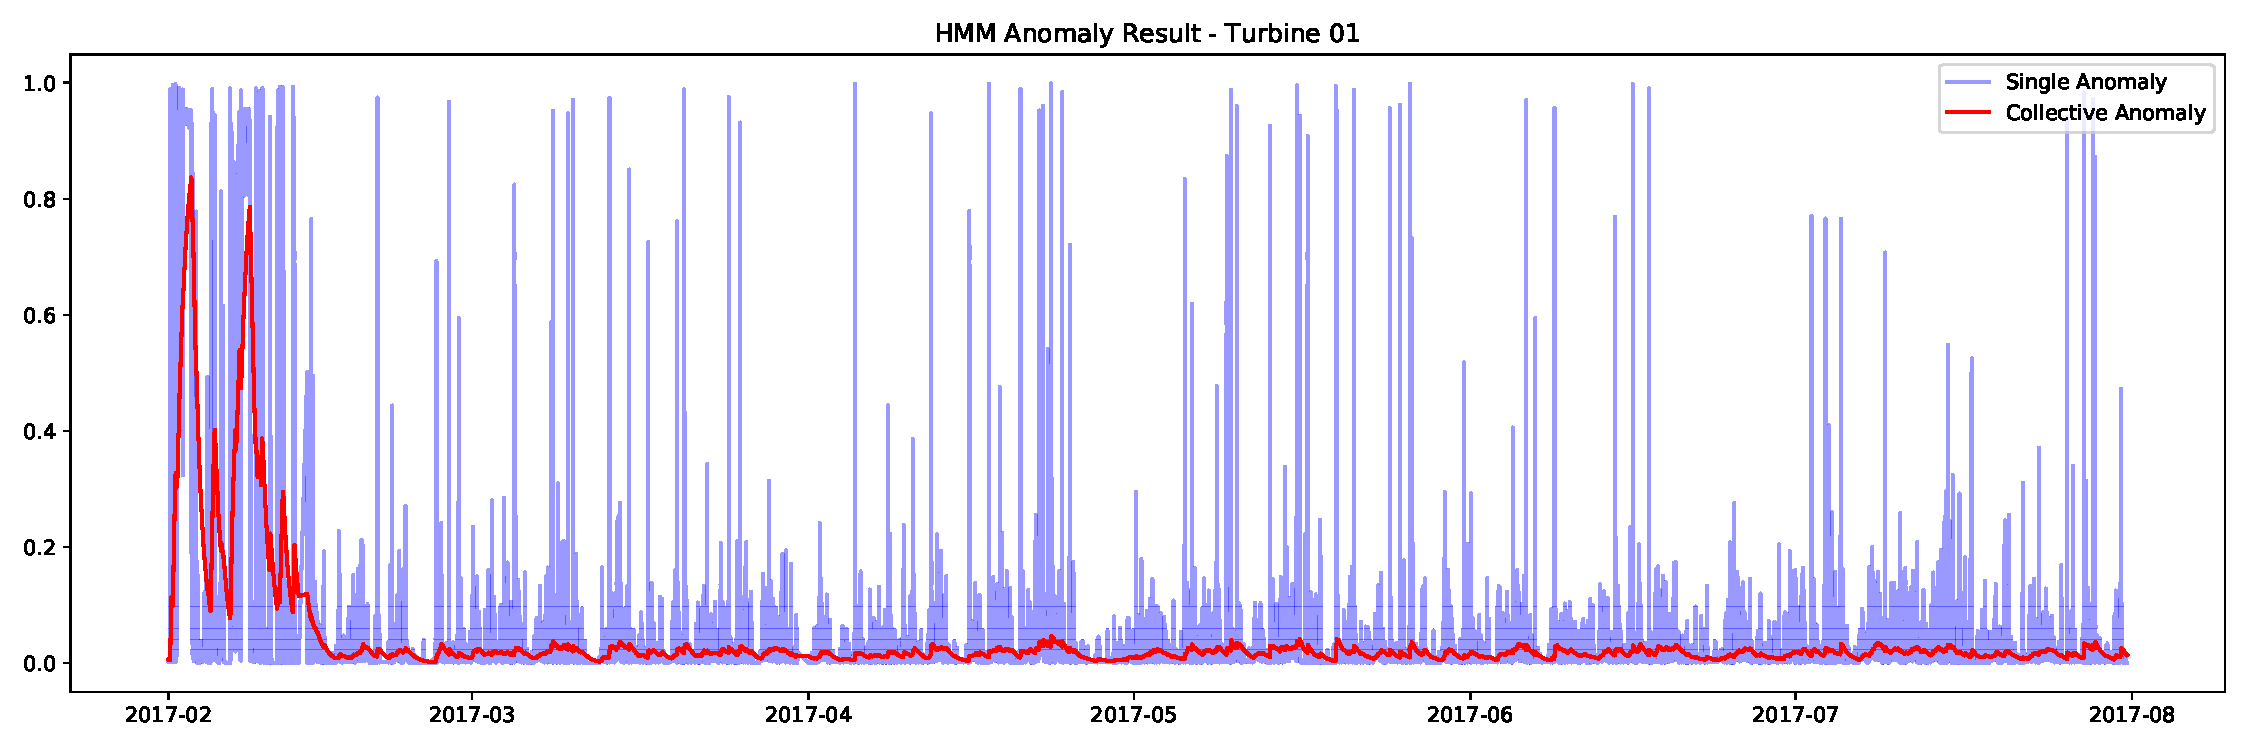
\includegraphics[width=0.48\textwidth]{hmm_t1.pdf}
       \label{fig:hmm-figa}
    }%
  \hfill
  \subfigure[The error prediction of GMM on the turbine which work under normal conditions]{
       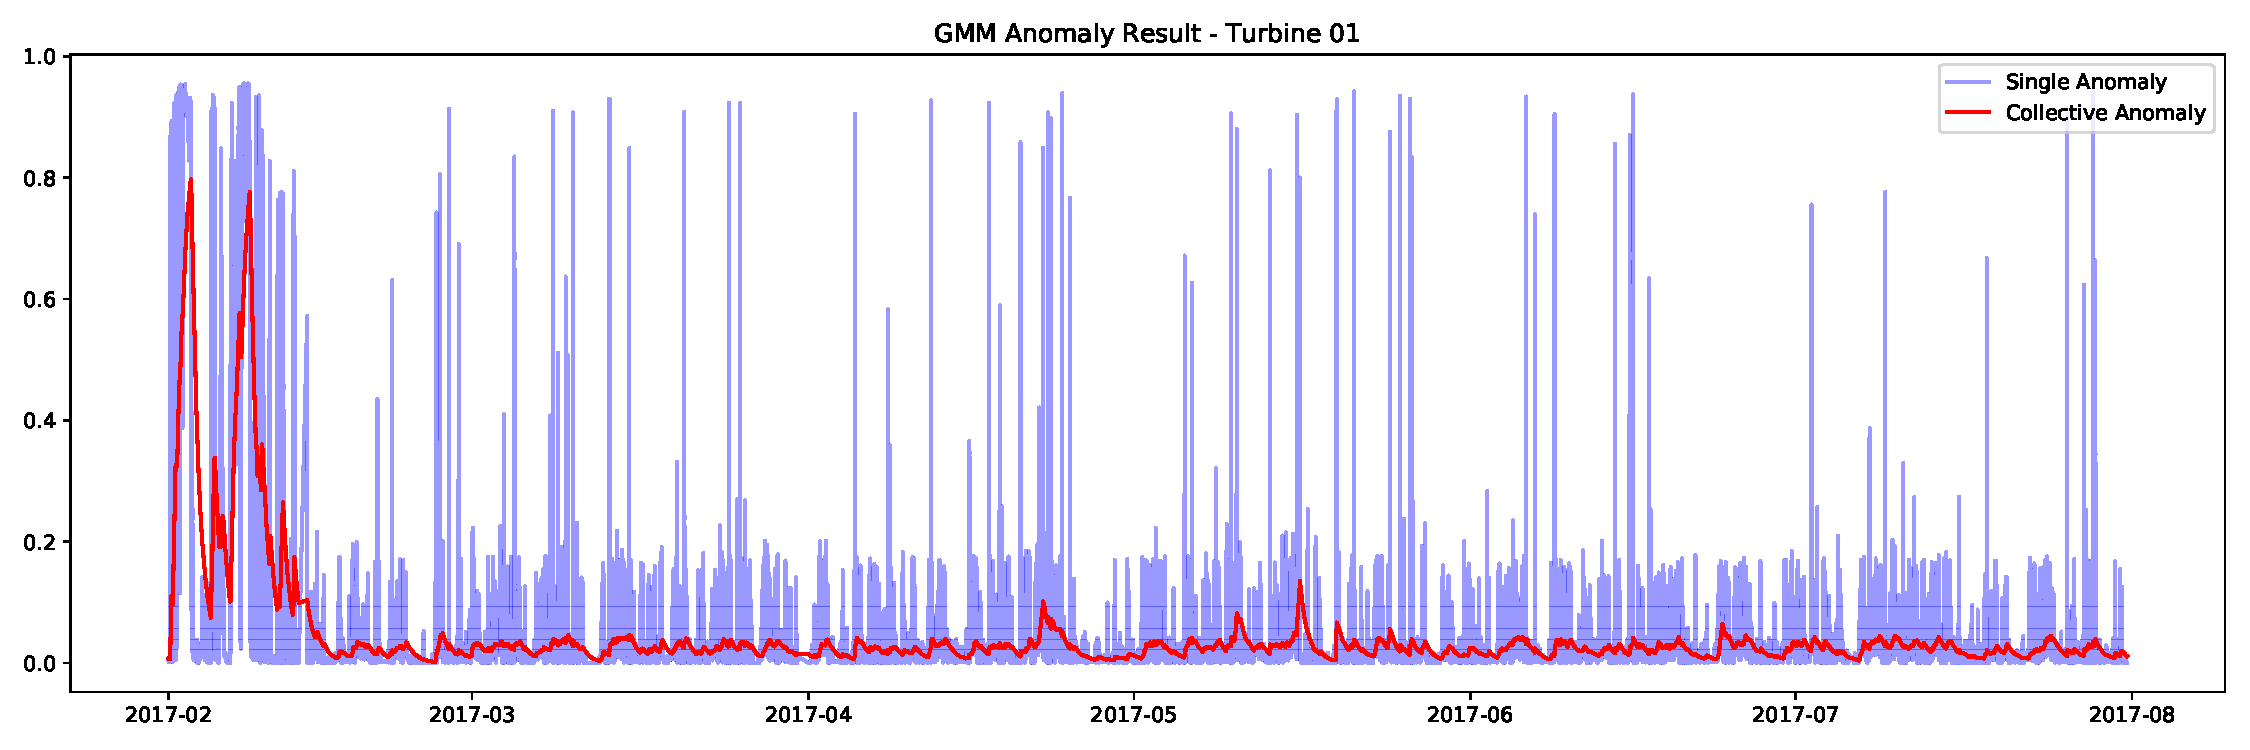
\includegraphics[width=0.48\textwidth]{gmm_t1.pdf}
       \label{fig:hmm-figb}
  }
  
  \subfigure[HMM generates two clear warning before malfunction on the June]{
       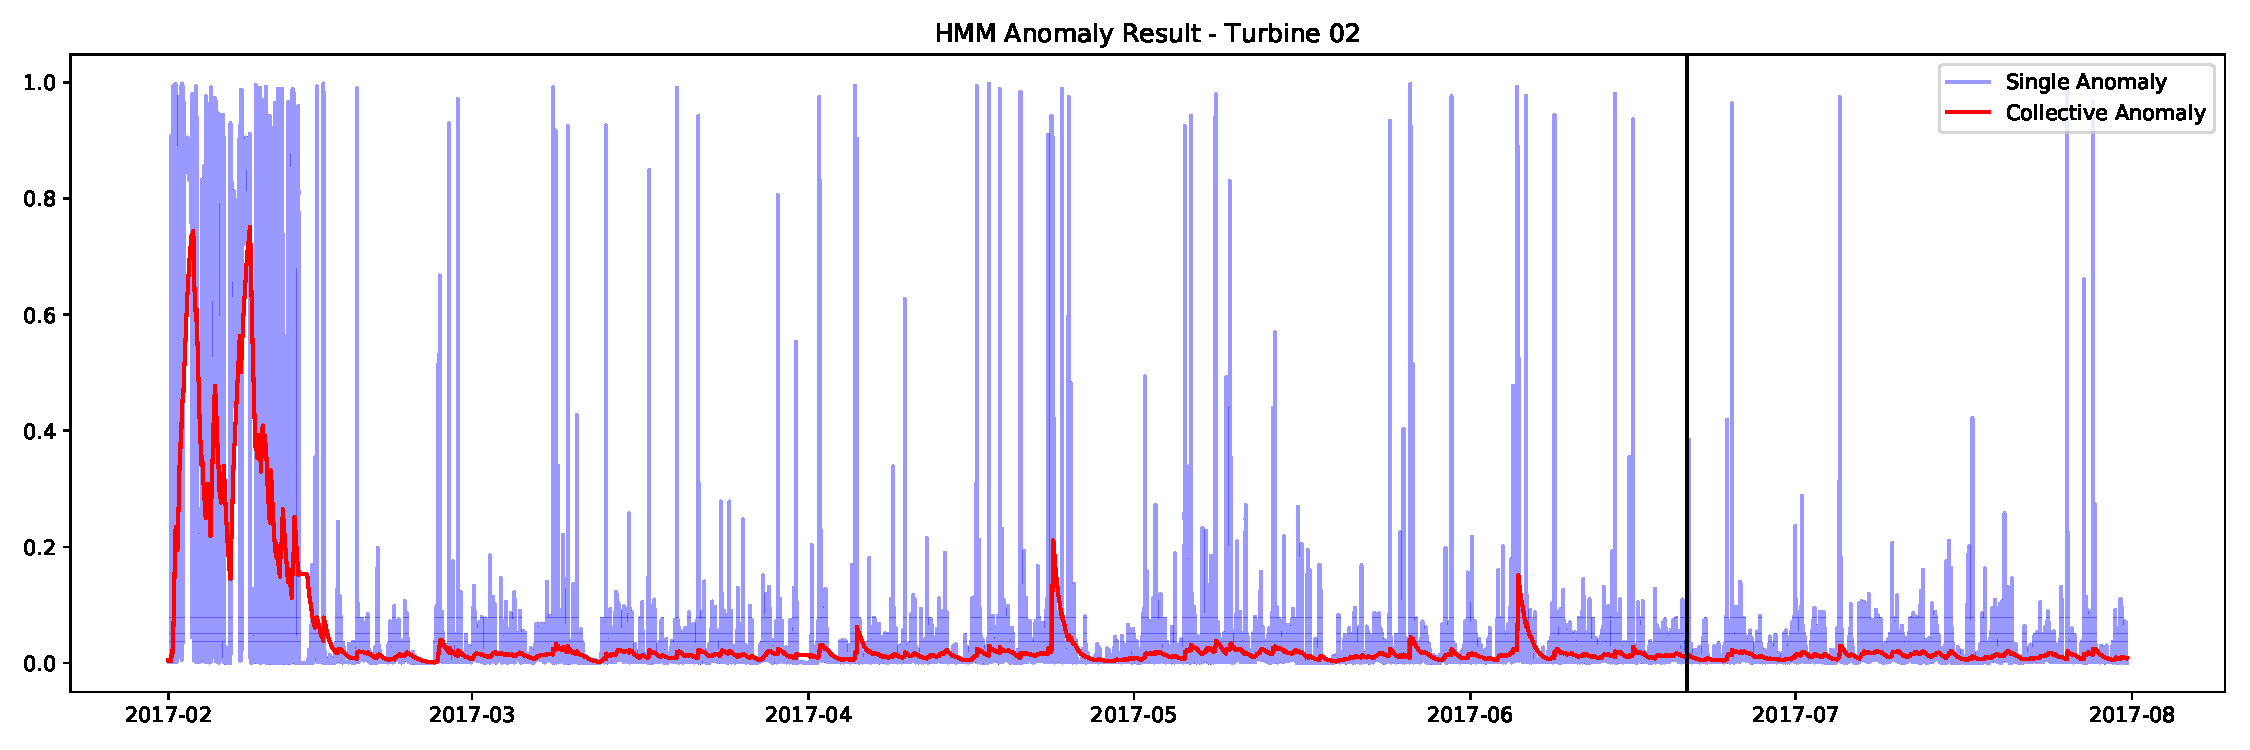
\includegraphics[width=0.48\textwidth]{hmm_t2.pdf}
       \label{fig:hmm-figc}
  }%
  \hfill
  \subfigure[Warnings of GMM are not clear as warning generated by HMM]{
       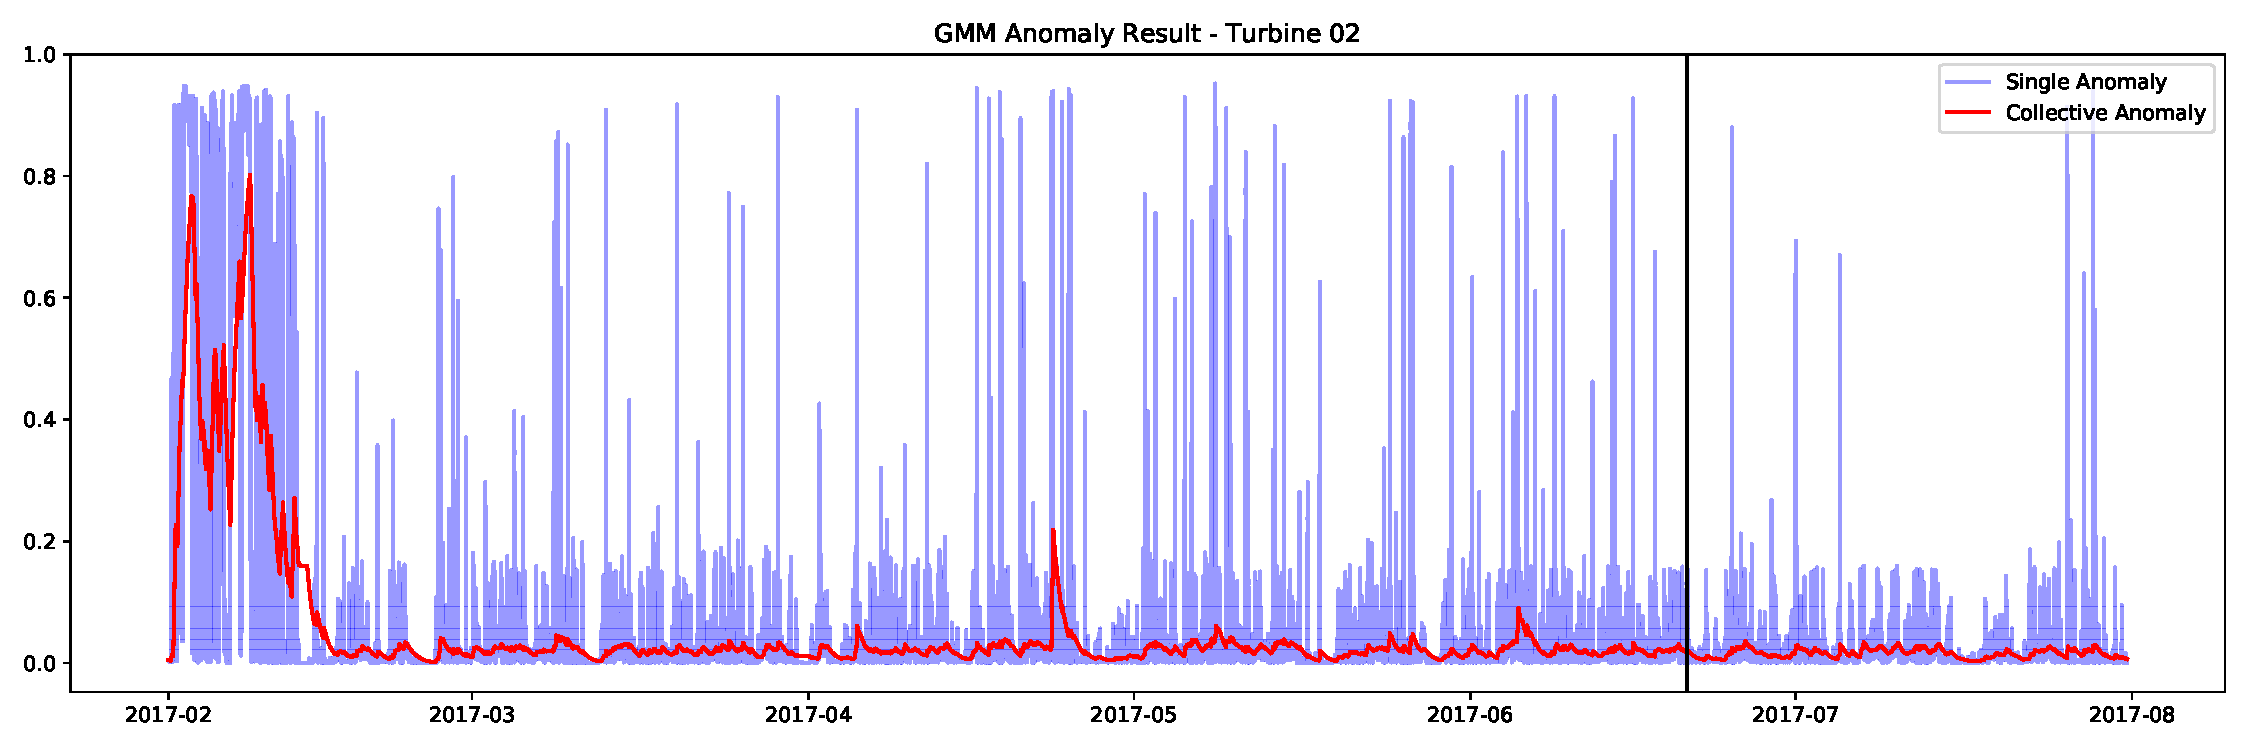
\includegraphics[width=0.48\textwidth]{gmm_t2.pdf}
        \label{fig:hmm-figd}
  }
  
  \subfigure[HMM does not predict error for the turbine which works under normal conditions]{
       %\centering
       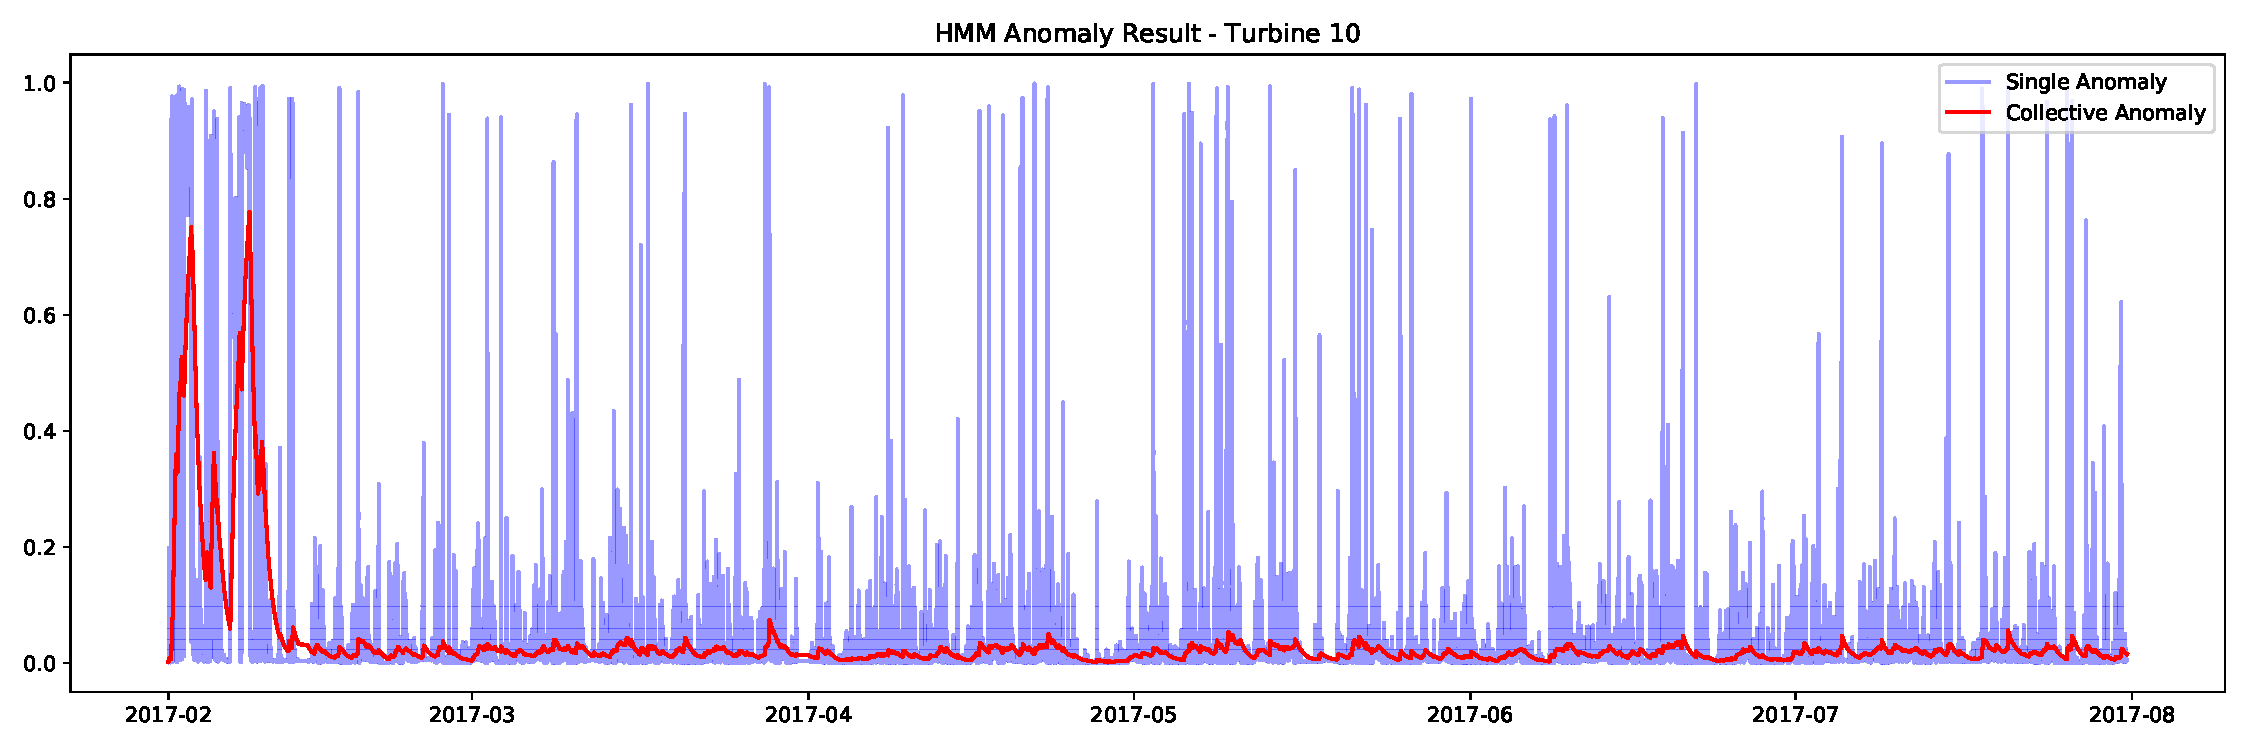
\includegraphics[width=0.48\textwidth]{hmm_t10.pdf}
        \label{fig:hmm-fige}
  }%
  \hfill
  \subfigure[GMMs tend to produce false positive warnings on the normally working turbine]{
       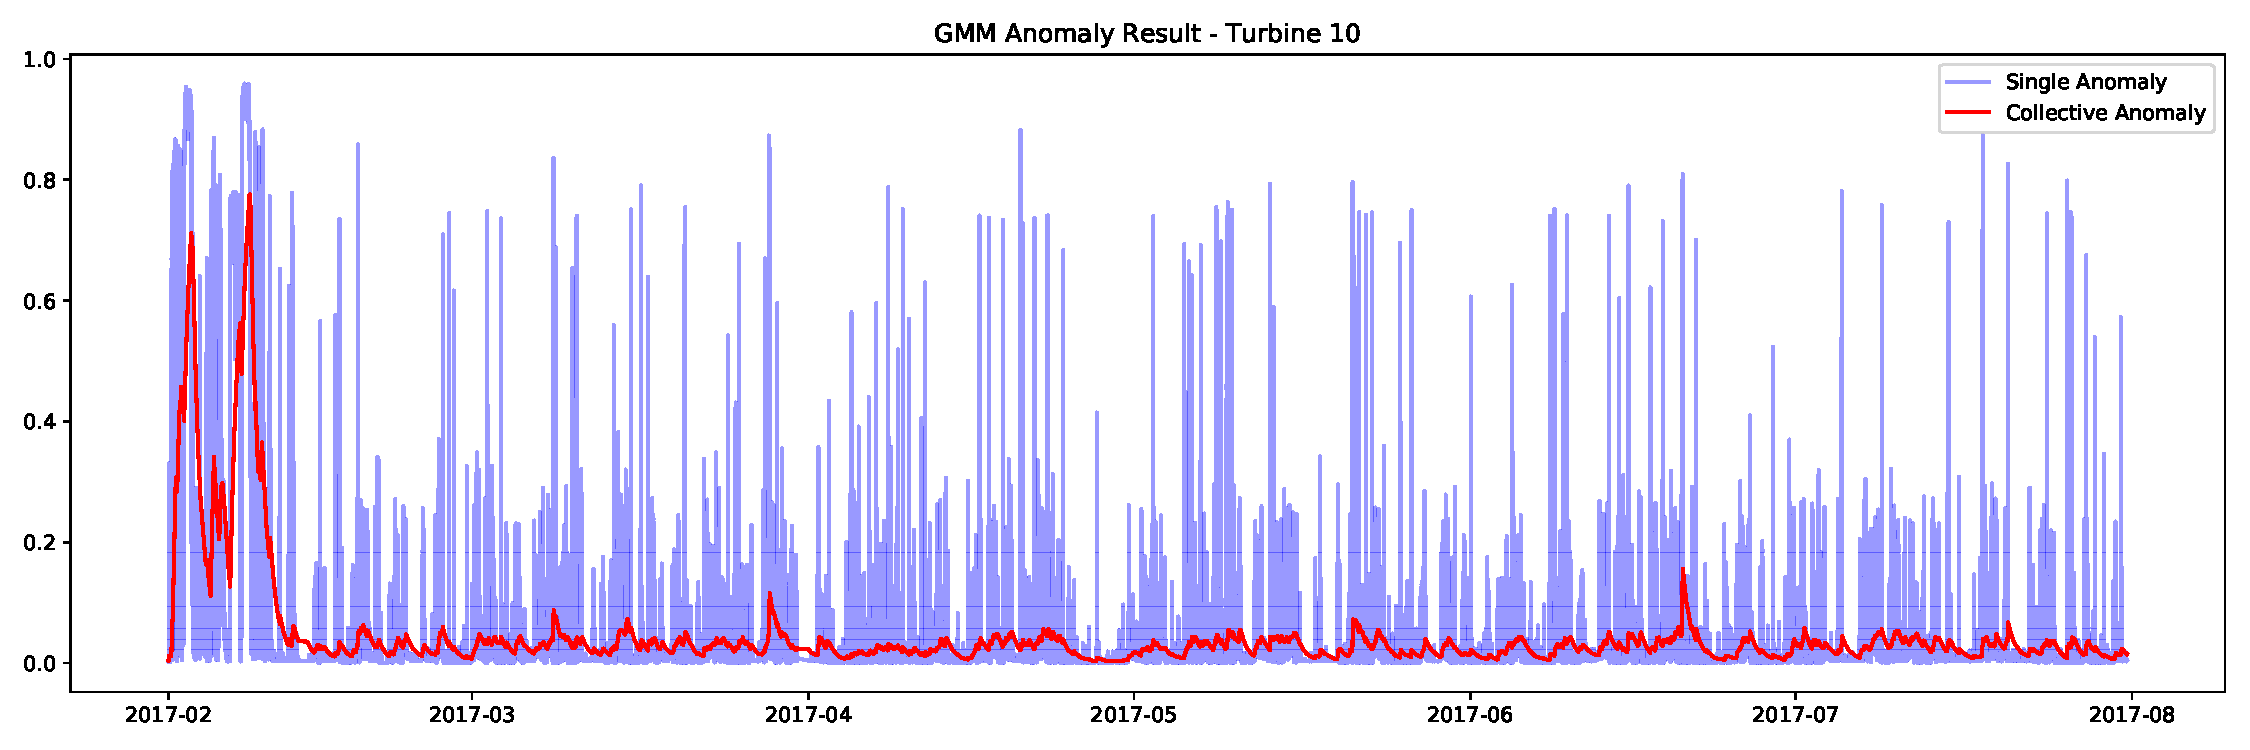
\includegraphics[width=0.48\textwidth]{gmm_t10.pdf}
       \label{fig:hmm-figf}
  }
  \caption{Comparison of the performance of HMM with GMM}
  \label{fig:hmm-results}
\end{figure}

\subsection{Experiments with the Deep Learning Sequence Models}

In this part of the study, we are interested in deep learning models to detect anomalies. 
Therefore we apply such models to the power curve of the wind turbines to learn about the system dynamics.
The main idea behind this study is to reconstruct the power curve of the wind turbines with developed models.
Then, in the test phase, we will first reconstruct the power curve, and compare this reconstruction with the new observations and measure how wrong they are.
This measurement will also determine our anomaly score.
In the experimental setup, we basically compare the RNN network with LSTM network.
While making this comparison, we will do our experiments by changing two additional parameters.
The first parameter to examine the effect on the model is the depth of the network.
For both RNN and LSTM, we compare the results with $1$-layer network with $2$-layer network (stacked) \cite{malhotra2015long}.
The other parameter to examine the effect on the model is loss function.
We examine the effect of the L1 loss and MSE loss on the developed model.
We focus on these two losses because both models have the rectified linear output layer, and these loss functions are more appropriate for such a model. 
In the rest of the experimental setup, we set all hyperparameters to the same for the healthy comparison.
We set learning rate $\eta = 0.01$ for all of the network setups, and we train each network for $1000$ number of the epoch. All the experimental setups use the same batch size, $144$ observation time-step for one batch. In the experiments, both RNN and LSTM network has the number of hidden layer size $128$.

\begin{figure}
\centering
    \subfigure{
        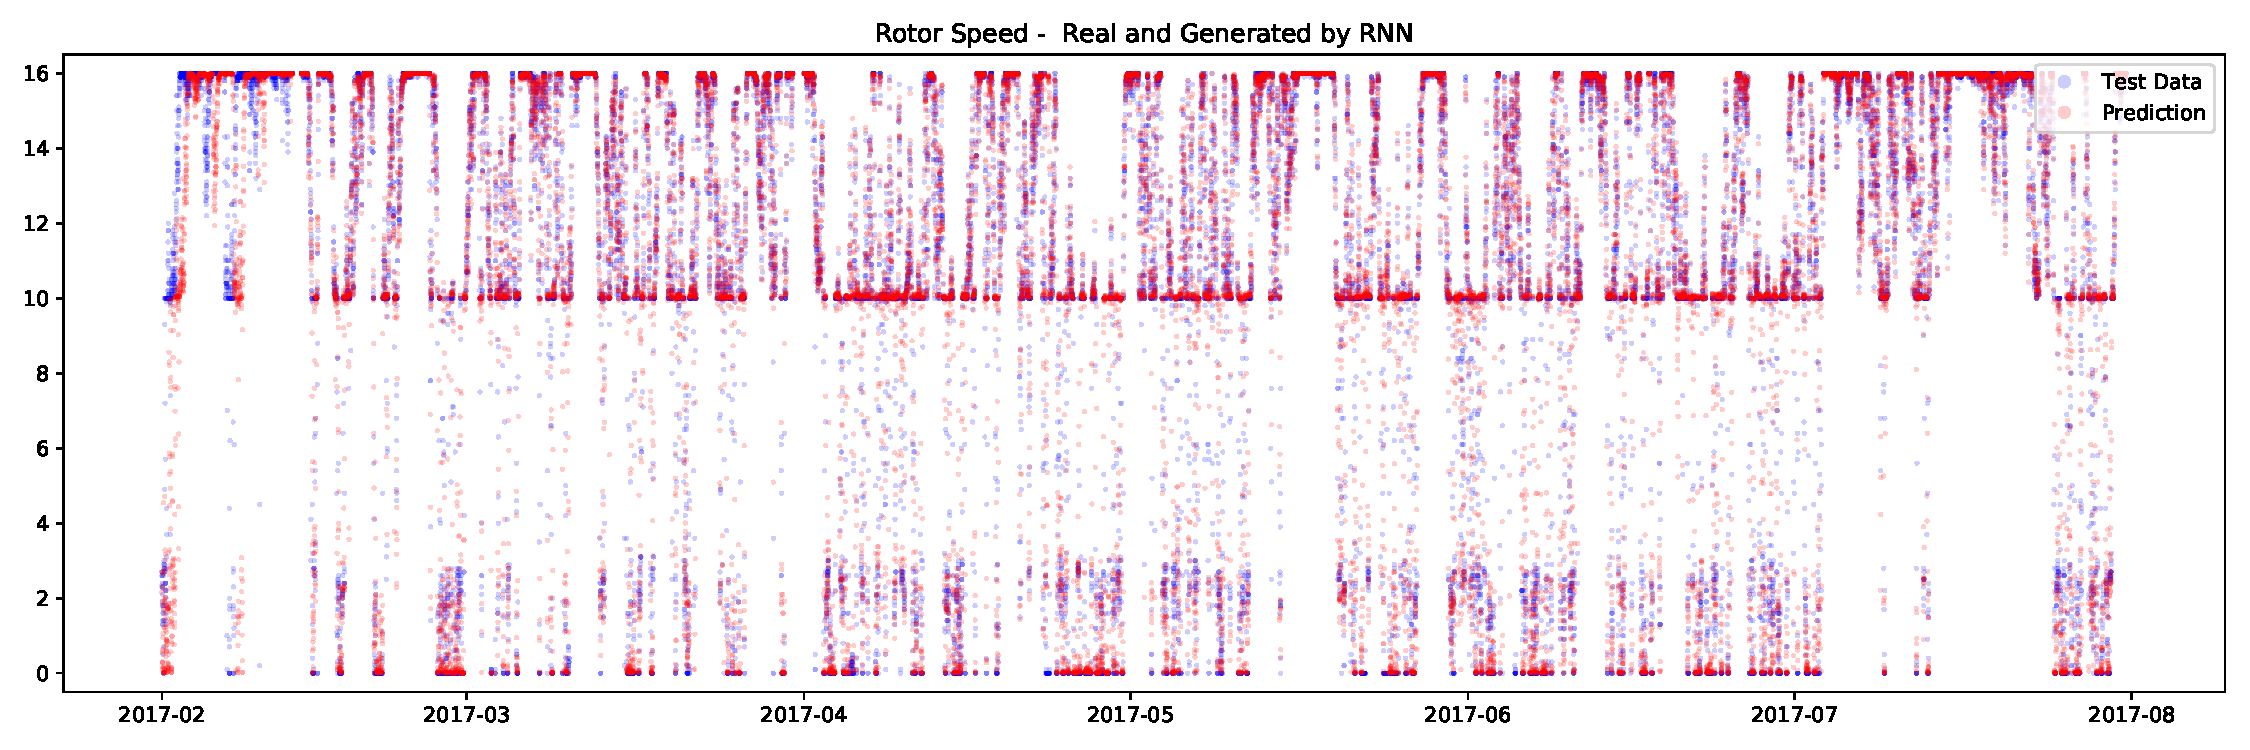
\includegraphics[width=0.9\textwidth]{rnn_rotor_128_2_tukey.pdf}
        \label{fig:rnn_rotor}
    }%
    
    \subfigure{
        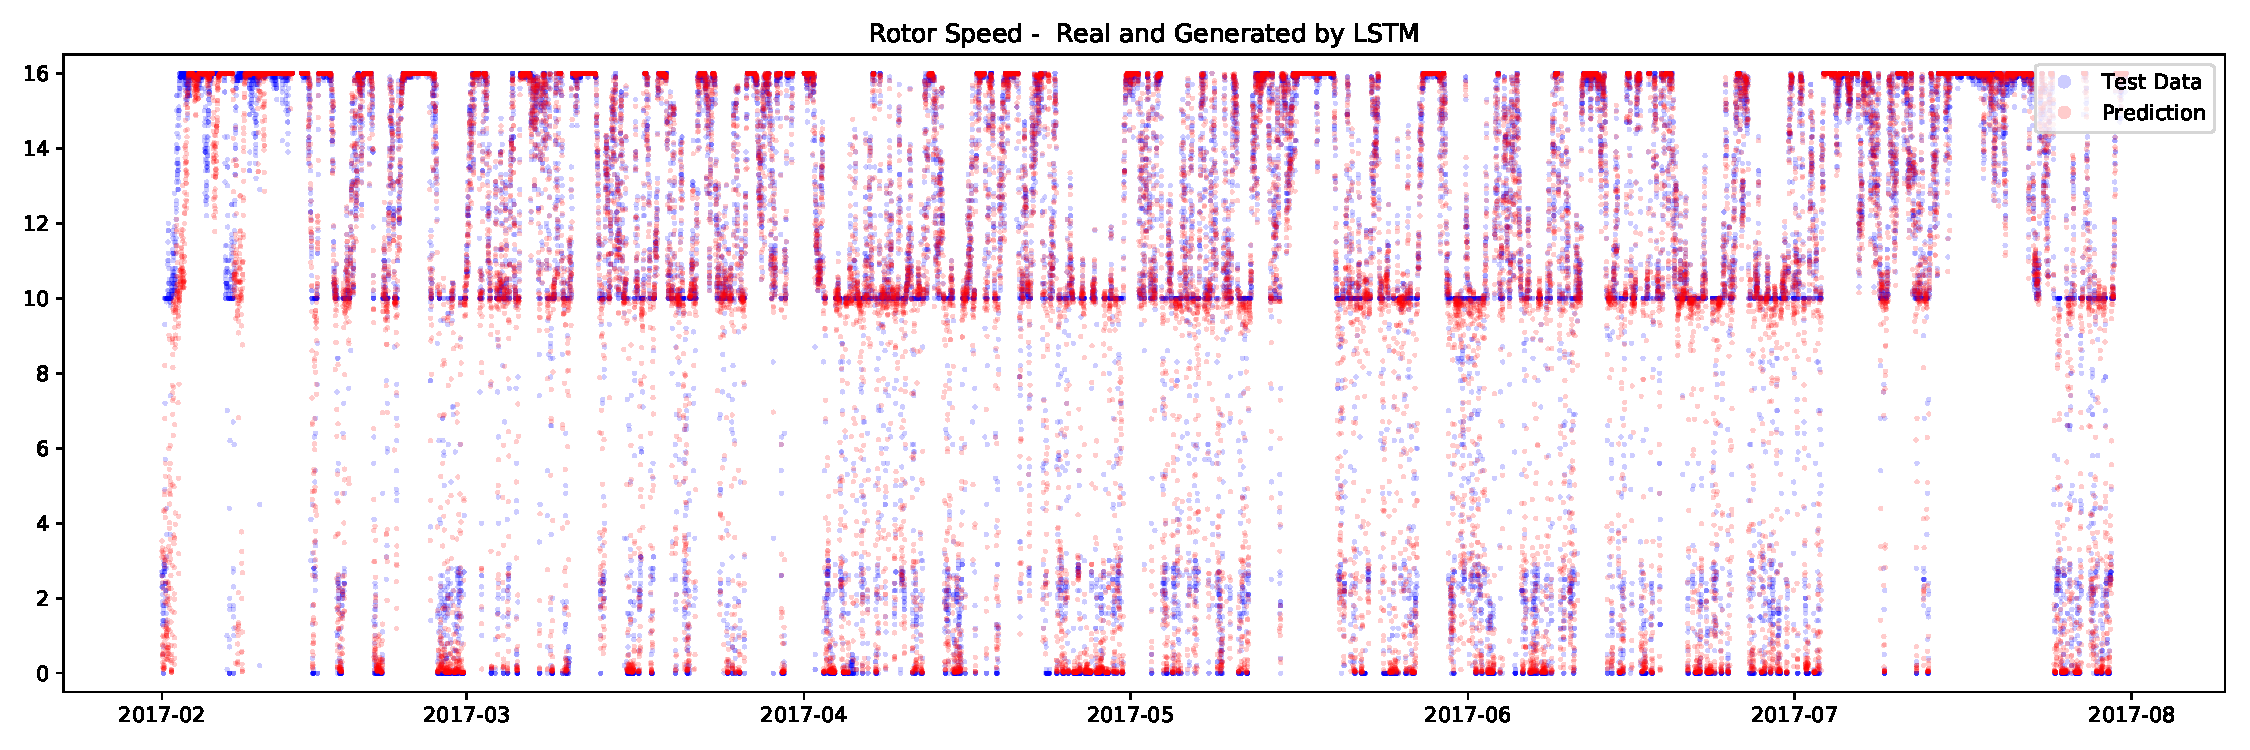
\includegraphics[width=0.9\textwidth]{lstm_rotor_128_2_tukey.pdf}
        \label{fig:lstm_rotor}
    }
    
    \caption{Predicted rotor speed data for RNN and LSTM model with Tukey's biweight loss}
    \label{fig:deep_rotors}
\end{figure}

In these experiments, we implement $12$ different experiment setup. 
These setups include RNN or LSTM, $1$-layer or $2$-layer, and L1 loss or MSE loss or Tukey's biweight loss.
Our experiments show that both RNN and LSTM setups have almost similar performance on the system.
This is because wind turbine dataset does not contain long-term dependencies and to obtain good estimation we do not need to know information from the future. 
On the other side, experiments show us that stacked networks perform better on the power curves.
This situation may be due to the complexity of the power curve.
Finally, we see in the experiments that L1 loss is a better choice to model such data because data includes anomalous observations and MSE loss not robust for such observations while L1 does.
Tukey's biweight loss, on the other hand, allow us to perform more robust optimizations and perform better on our task.
These networks almost totally correctly estimate the generated power and rotor speed values from the given wind speed, as in Figure~\ref{fig:deep_rotors}, Figure~\ref{fig:deep_powers}, Figure~\ref{fig:1-deep_power_curves} and Figure~\ref{fig:2-deep_power_curves}. 
The first two figures are generated from the stacked RNN and stacked LSTM network with the Tuckey's biweight loss.
Except for a small difference, both the RNN and LSTM model creates almost the same predictions on rotor speed and grid power values.
The third figure includes generated power curves for all experimental setups. In all figures, blue dots represent the observations while red dots show the model outputs.
In Figure~\ref{fig:1-deep_power_curves}, one can detailly analyze the performance of the 1-layer models with a different setting.
Similarly, in Figure~\ref{fig:2-deep_power_curves}, we share the performance of stacked (2-layered) networks.
Despite their small differences, all models produced acceptable results and found almost the same anomaly result. The anomaly scores are shown in Figure~\ref{fig:1-deep_anomalies} and Figure~\ref{fig:2-deep_anomalies}. 
Black vertical lines in the figures represent the malfunction in turbines, and the system generates warning before the malfunction.
Additionally, we know that at the February there is an iciness on the turbines. 
Models successfully detect these anomalies in all experiments.
These figures show that the results are very similar to each other and also similar to the ones that we find with probabilistic models in Figure~\ref{fig:hmm-results}.
Detailed analysis of the 1-layer networks can be found in Figure~\ref{fig:1-deep_anomalies}, while Figure~\ref{fig:2-deep_anomalies} includes detailed analysis of the 2-layer (stacked) networks.
In both experiments, blue dots represent the observations while red dots represent the predictions.

\begin{figure}
\centering
    \subfigure{
        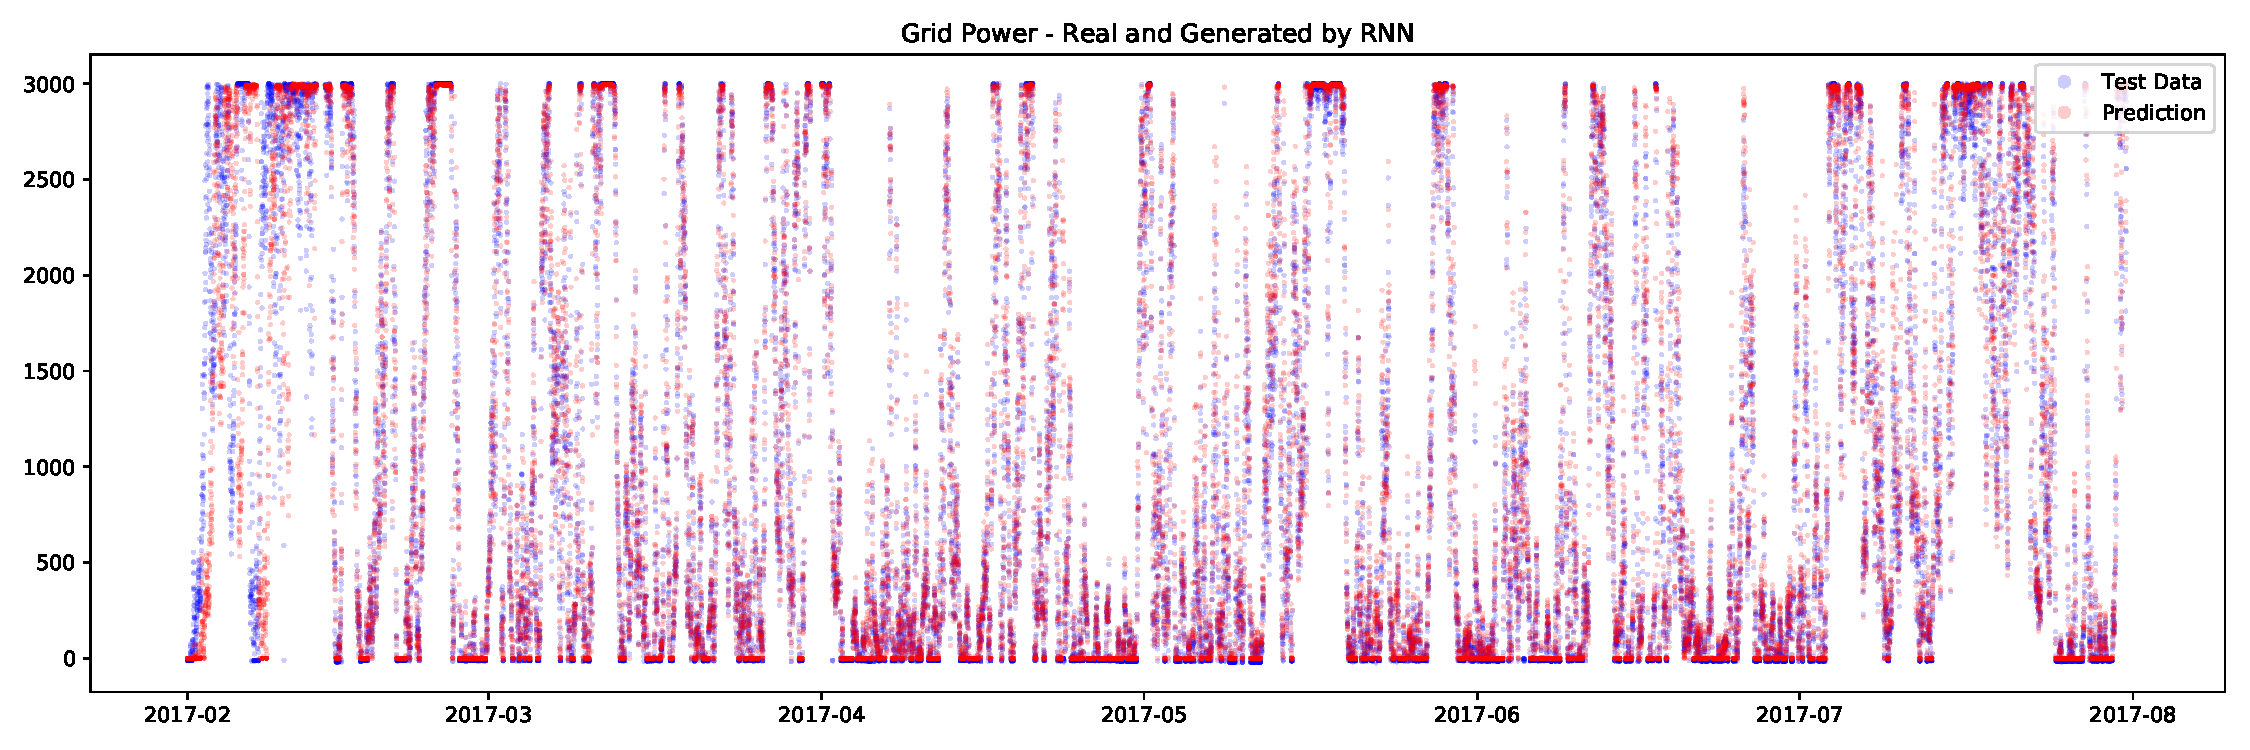
\includegraphics[width=0.9\textwidth]{rnn_grid_power_128_2_tukey.pdf}
        \label{fig:rnn_power}
    }%
    
    \subfigure{
        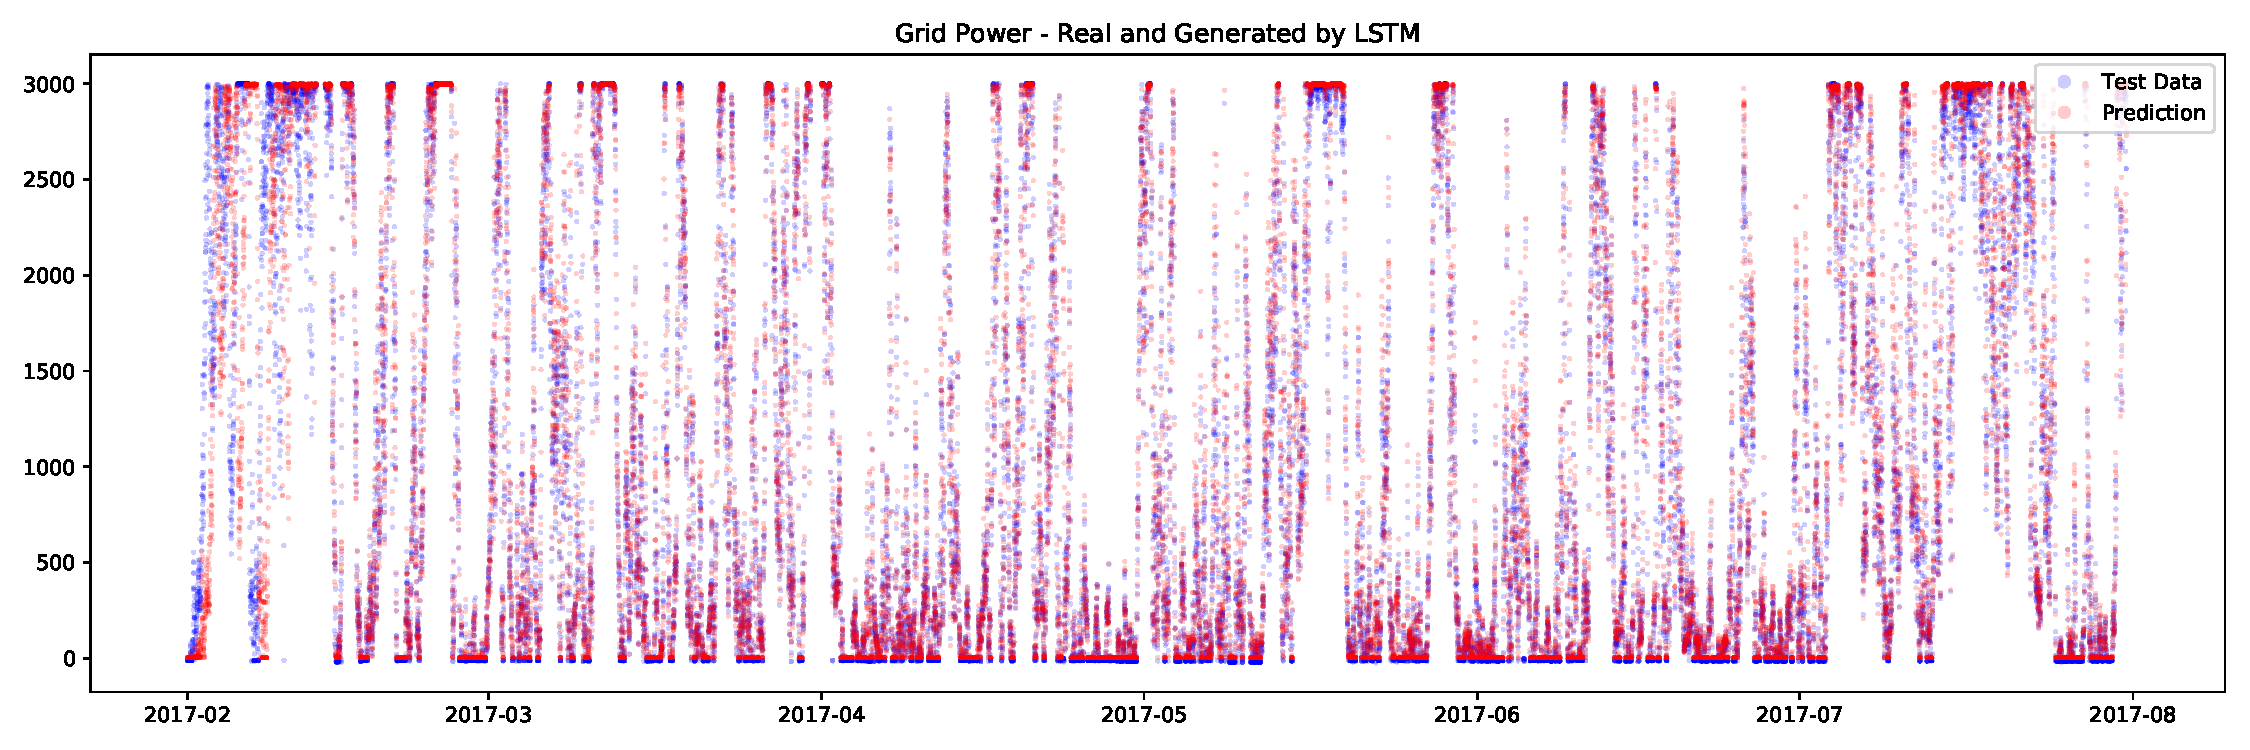
\includegraphics[width=0.9\textwidth]{lstm_grid_power_128_2_tukey.pdf}
        \label{fig:lstm_power}
    }
    
    \caption{Predicted generated power data for RNN and LSTM model with Tukey's biweight loss}
    \label{fig:deep_powers}
\end{figure}

\begin{figure}
    \centering
  \subfigure[RNN with MSE loss]{
       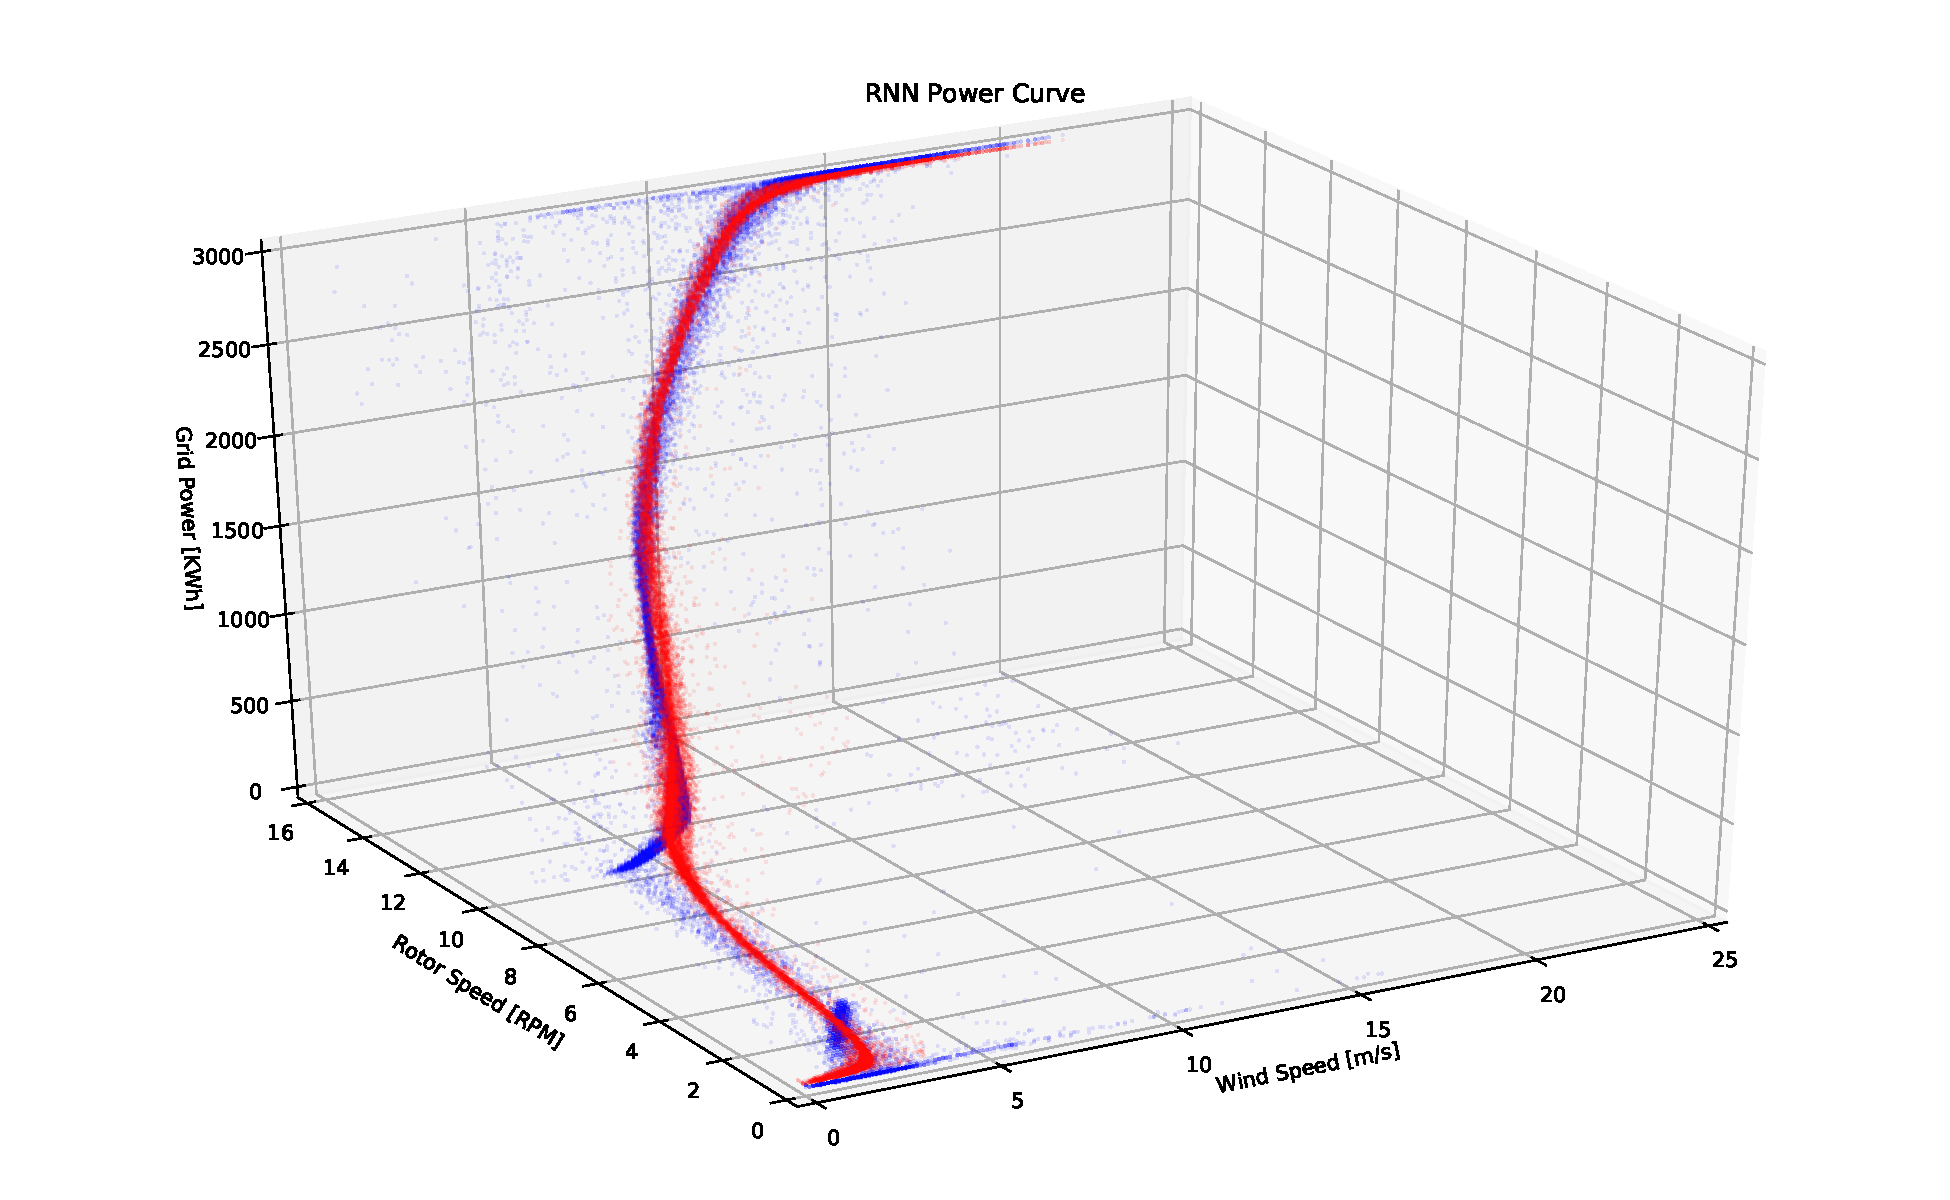
\includegraphics[width=0.47\textwidth]{rnn_power_curve_128_1_MSE.pdf}
       \label{fig:1-rnn-power_curve-figa}
    }%
  \hfill
  \subfigure[LSTM with MSE loss]{
       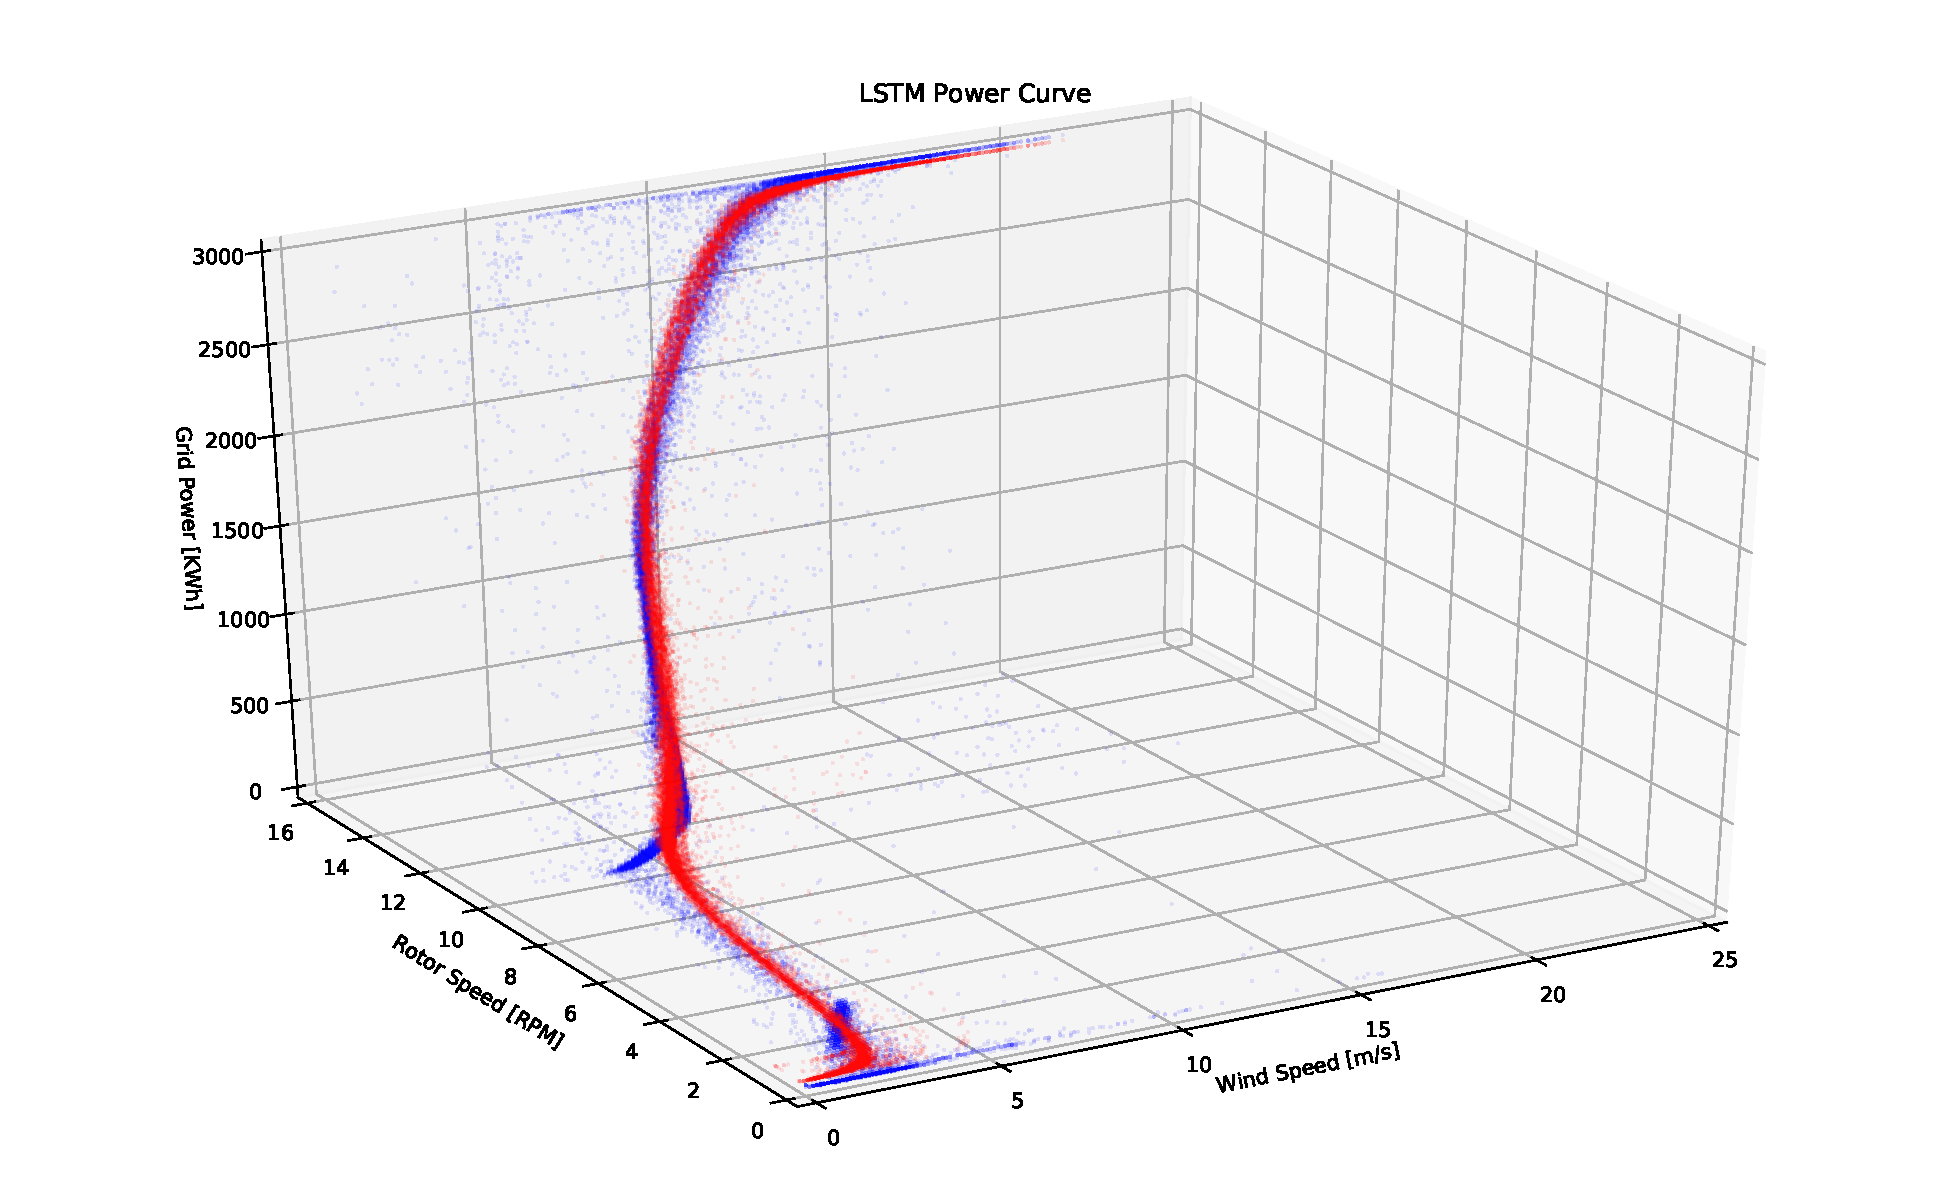
\includegraphics[width=0.47\textwidth]{lstm_power_curve_128_1_MSE.pdf}
       \label{fig:1-lstm-power_curve-figa}
  }
  
  \subfigure[RNN with L1 loss]{
       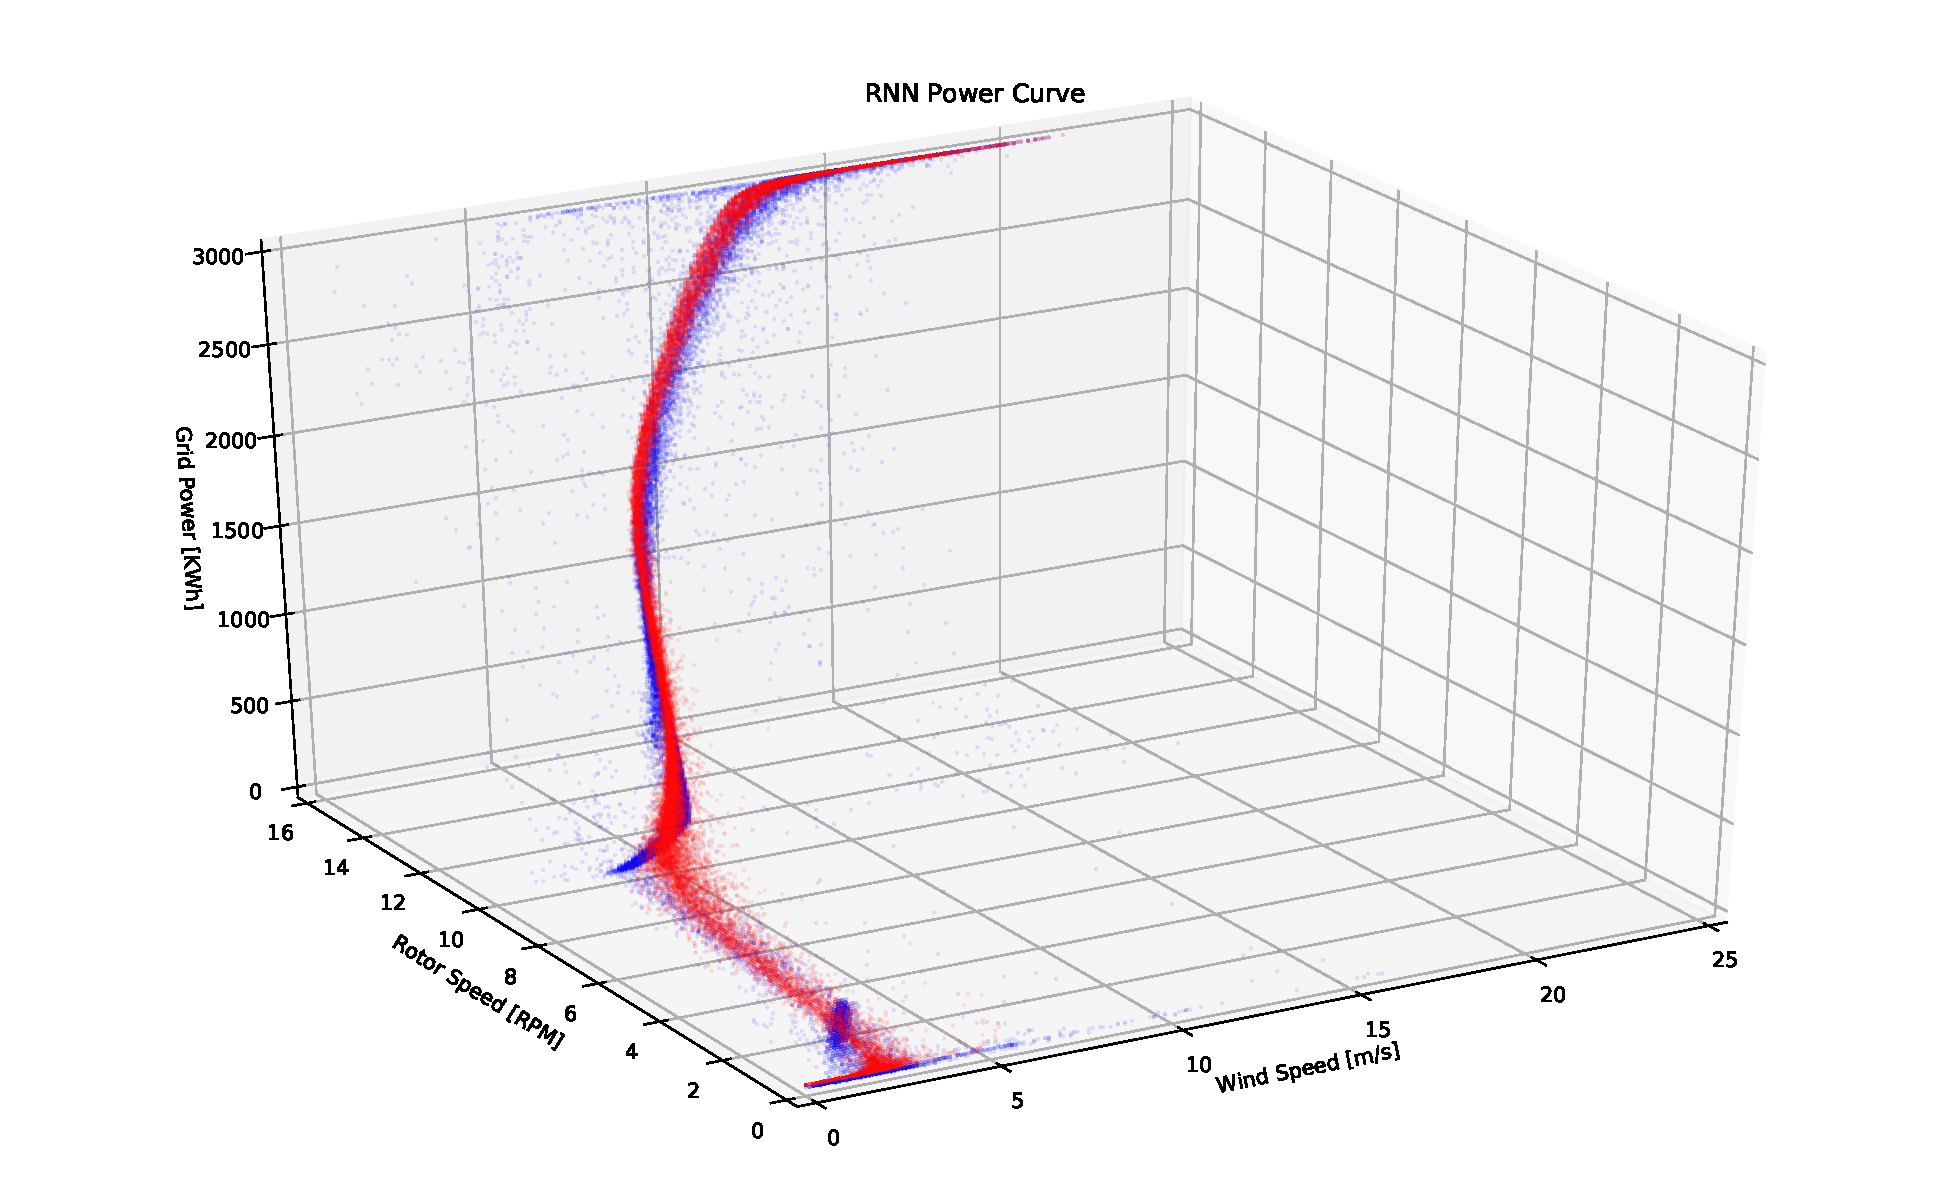
\includegraphics[width=0.47\textwidth]{rnn_power_curve_128_1_L1.pdf}
       \label{fig:1-rnn-power_curve-figb}
  }%
  \hfill
  \subfigure[LSTM with L1 loss]{
       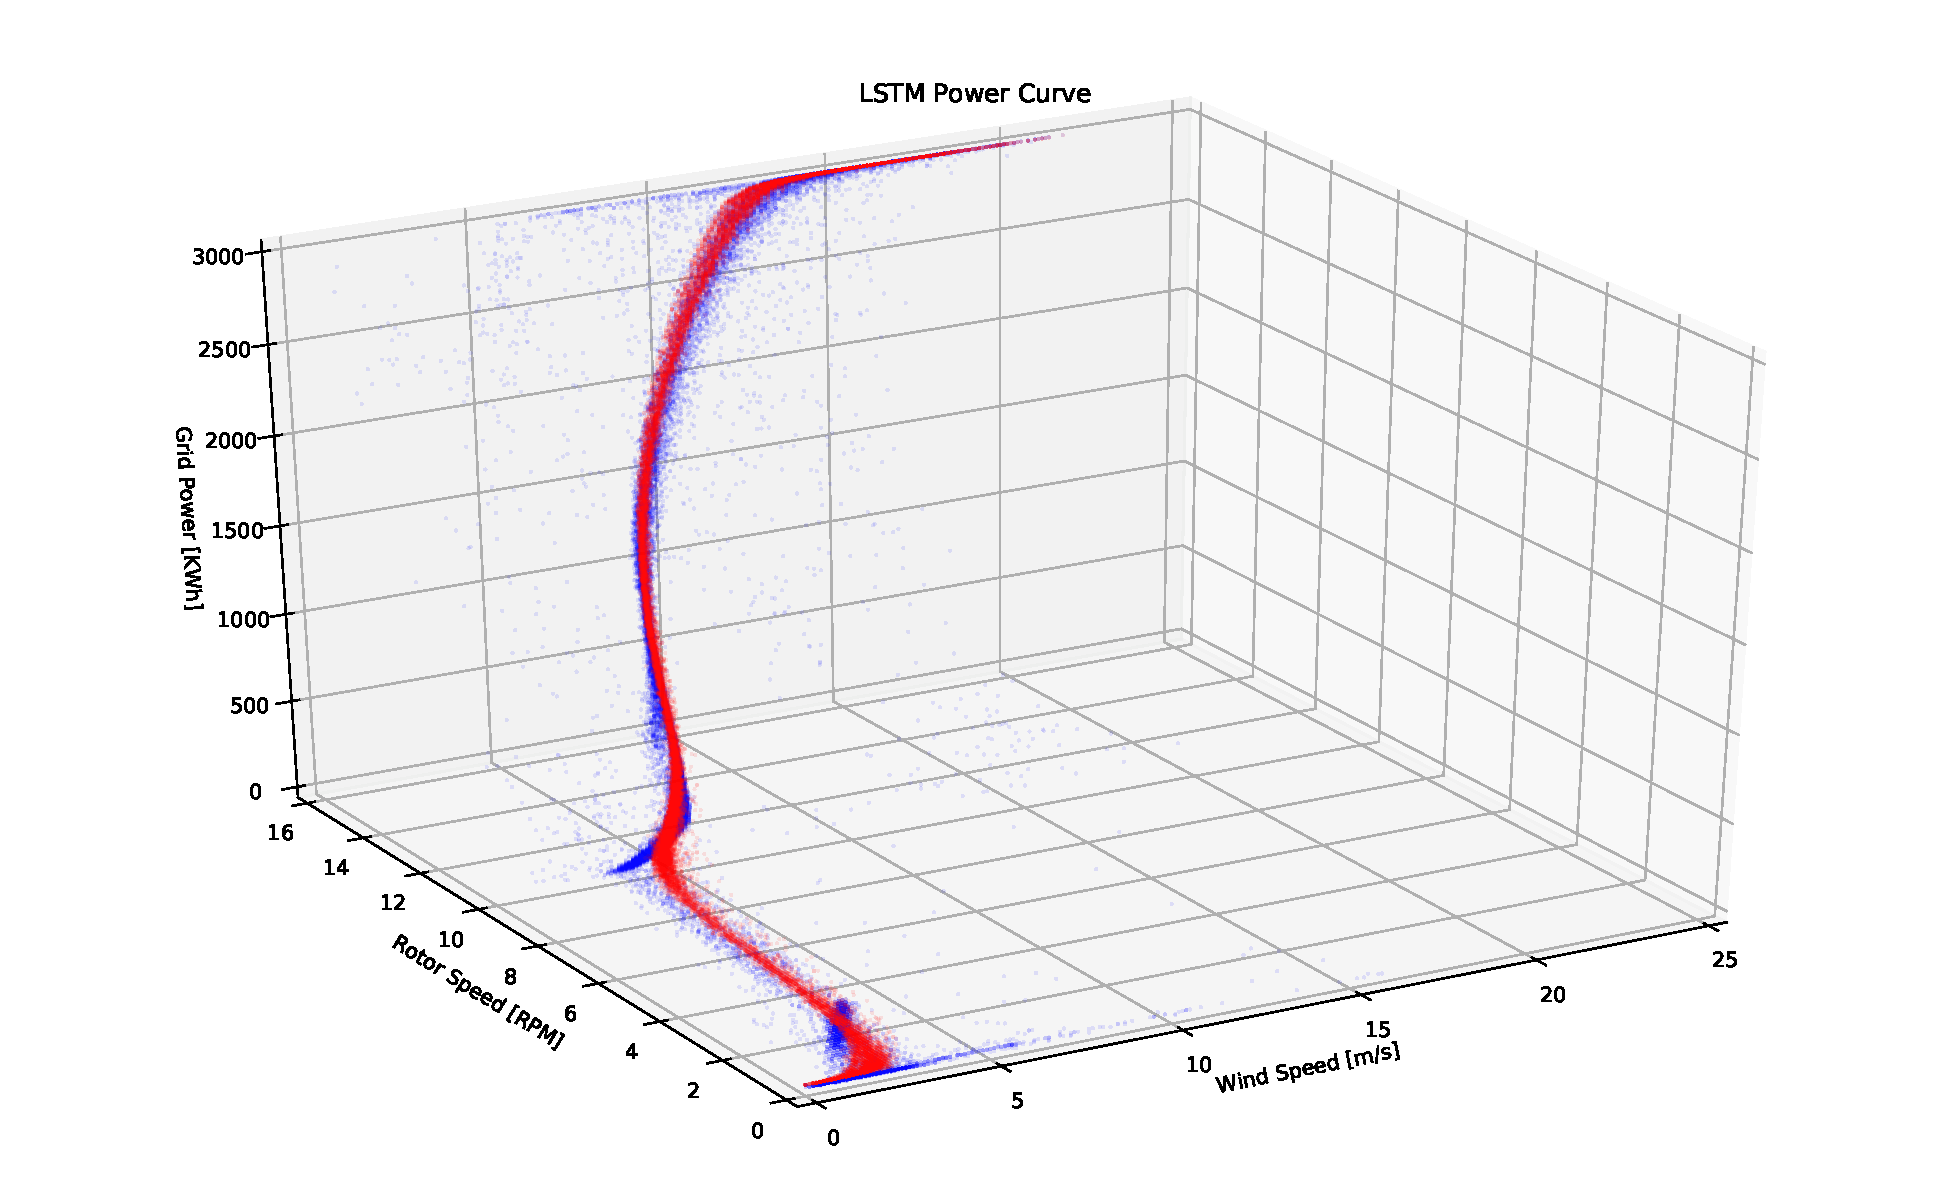
\includegraphics[width=0.47\textwidth]{lstm_power_curve_128_1_L1.pdf}
        \label{fig:1-lstm-power_curve-figb}
  }
  
  \subfigure[RNN with Tukey's biweight loss]{
       %\centering
       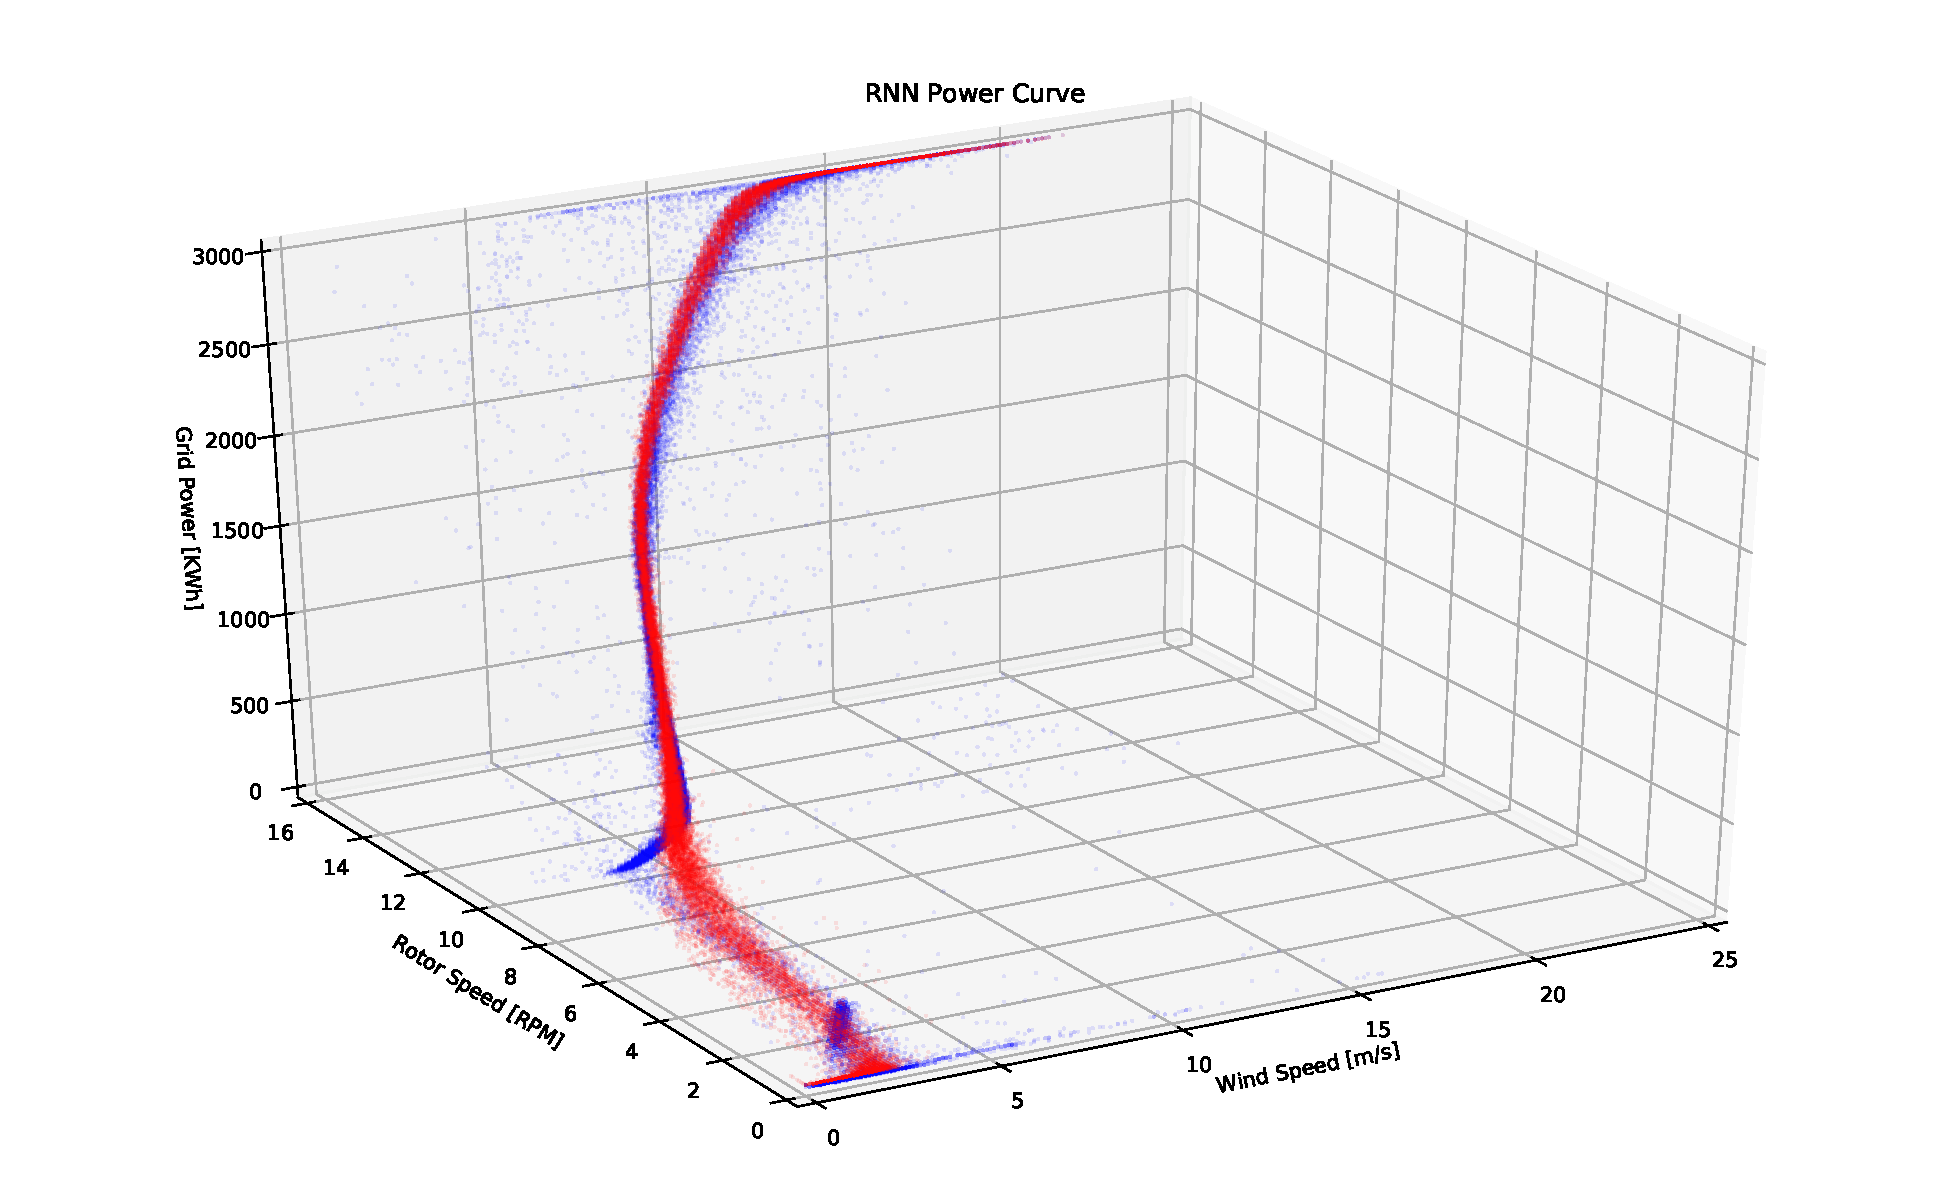
\includegraphics[width=0.47\textwidth]{rnn_power_curve_128_1_tukey.pdf}
        \label{fig:1-rnn-power_curve-figc}
  }%
  \hfill
  \subfigure[LSTM with Tukey's biweight loss]{
       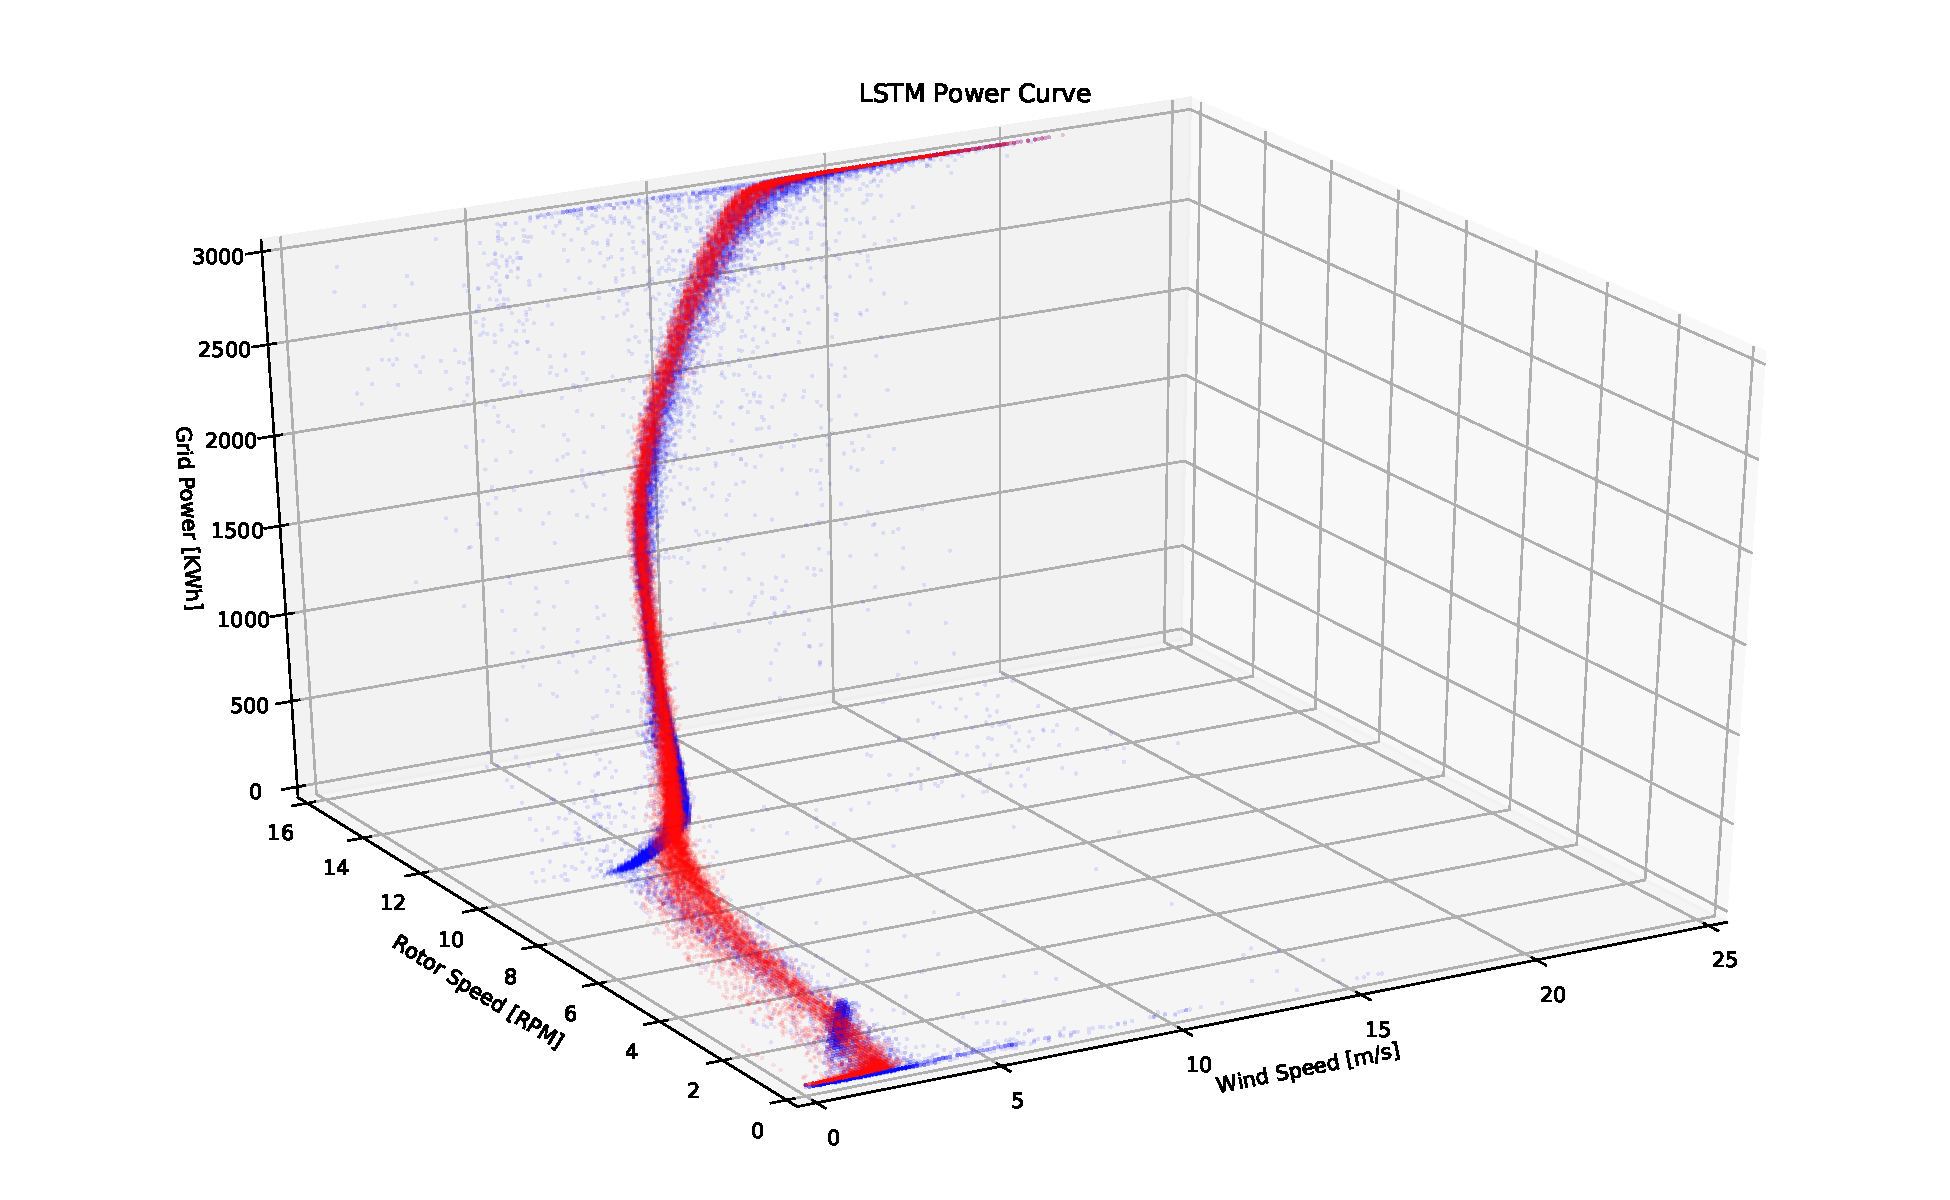
\includegraphics[width=0.47\textwidth]{lstm_power_curve_128_1_tukey.pdf}
       \label{fig:1-lstm-power_curve-figc}
  }
  \vspace{10pt}
  \caption{Generated from 1-layer network and observed power curves}
  \label{fig:1-deep_power_curves}
\end{figure}

\begin{figure}
    \centering
  \subfigure[RNN with MSE loss]{
       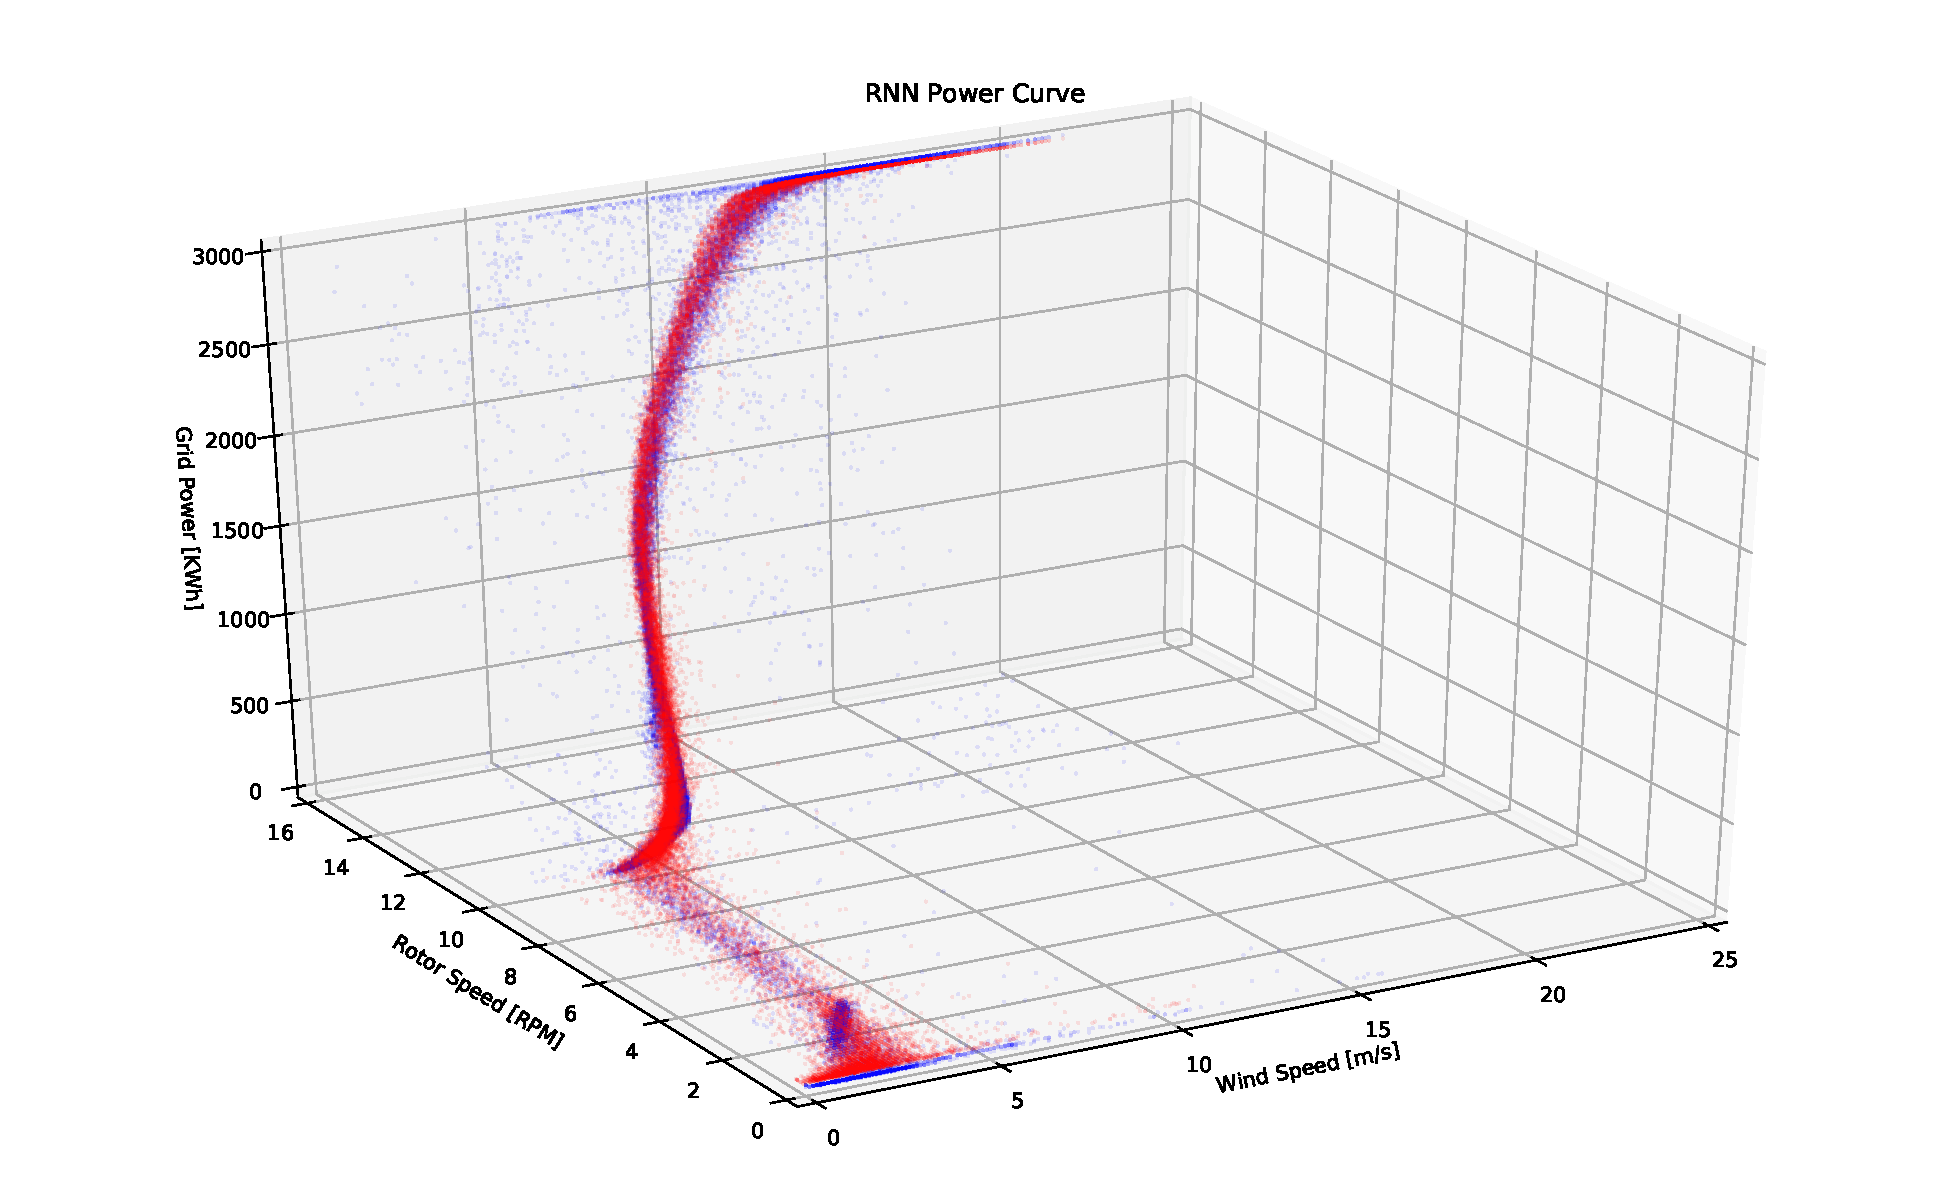
\includegraphics[width=0.47\textwidth]{rnn_power_curve_128_2_MSE.pdf}
       \label{fig:2-rnn-power_curve-figa}
    }%
  \hfill
  \subfigure[LSTM with MSE loss]{
       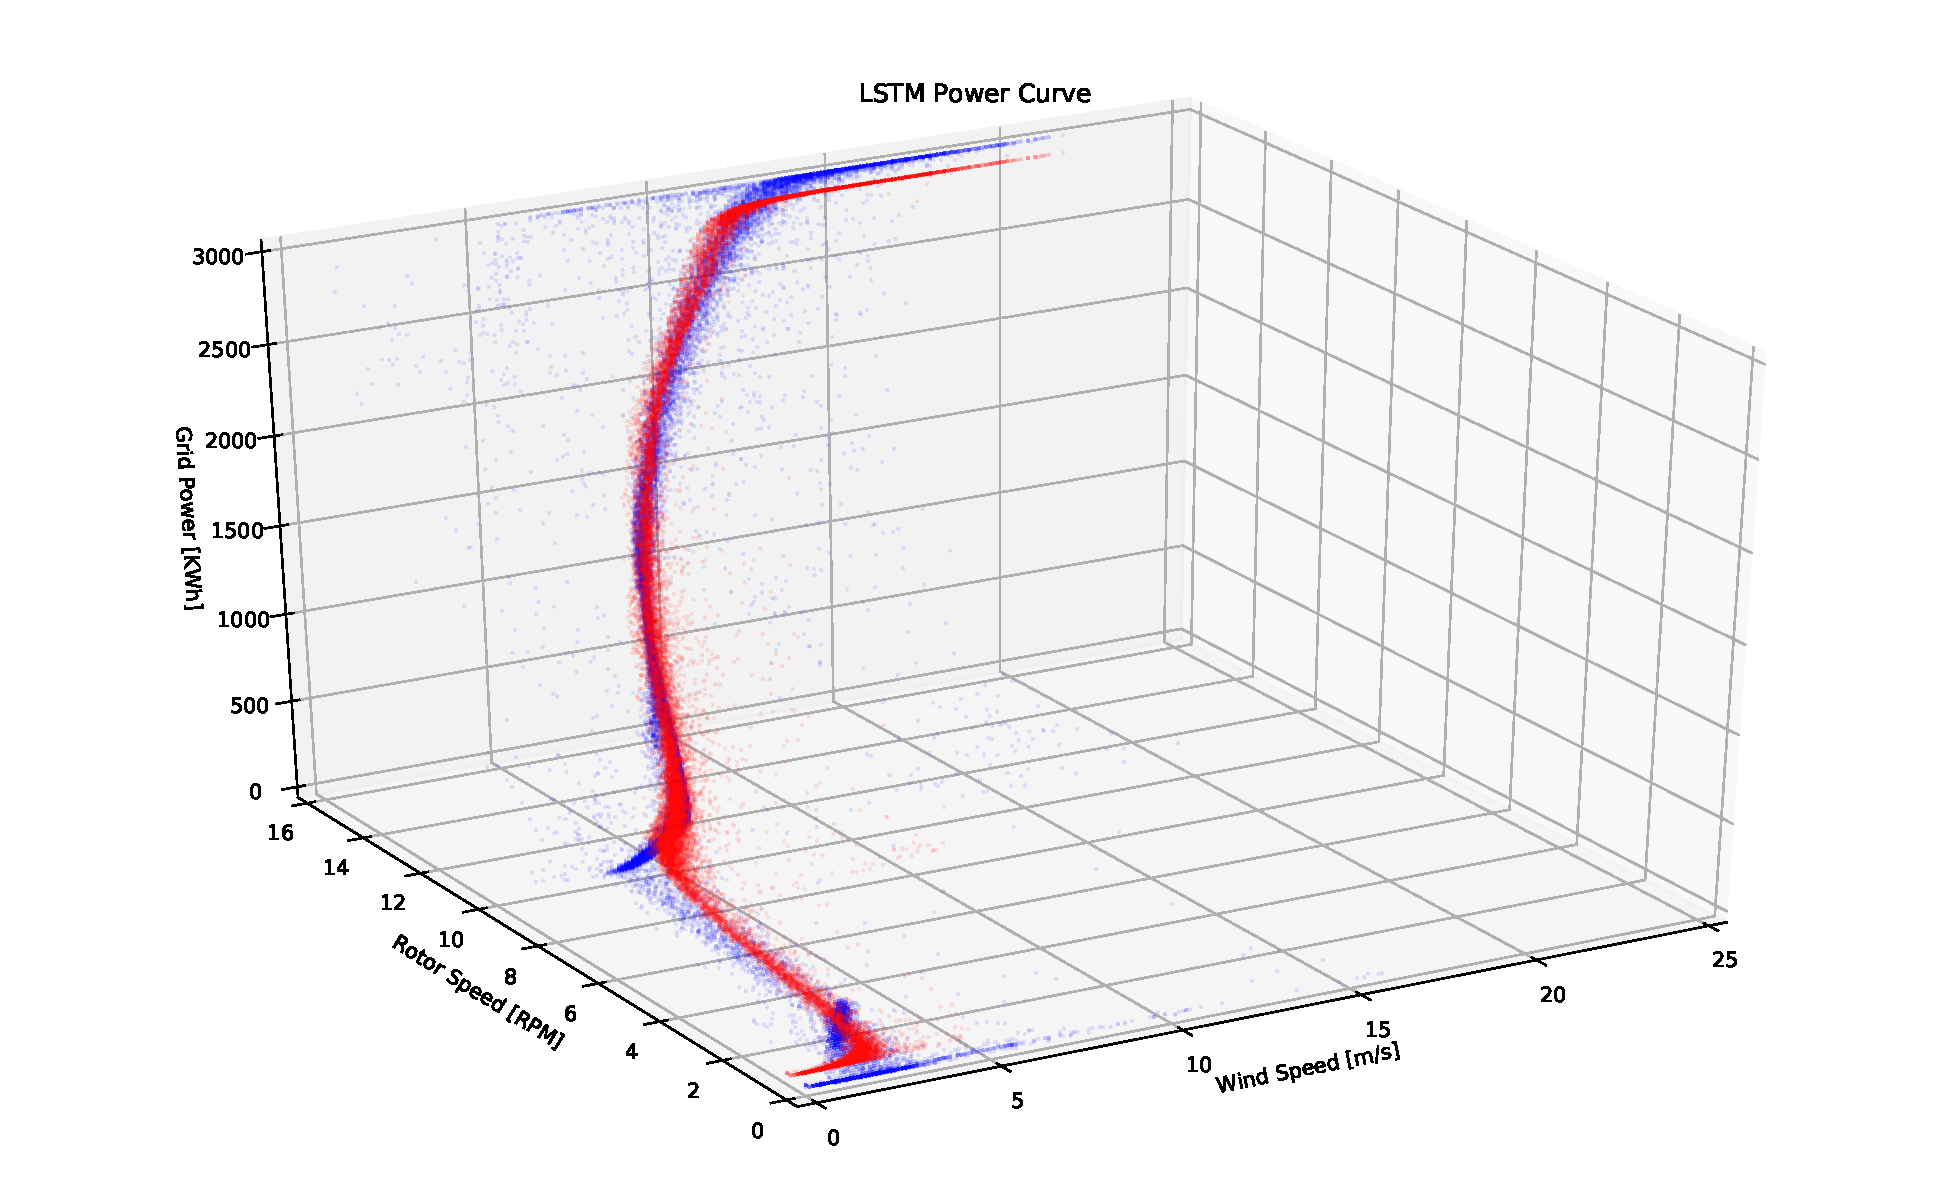
\includegraphics[width=0.47\textwidth]{lstm_power_curve_128_2_MSE.pdf}
       \label{fig:2-lstm-power_curve-figa}
  }
  
  \subfigure[RNN with L1 loss]{
       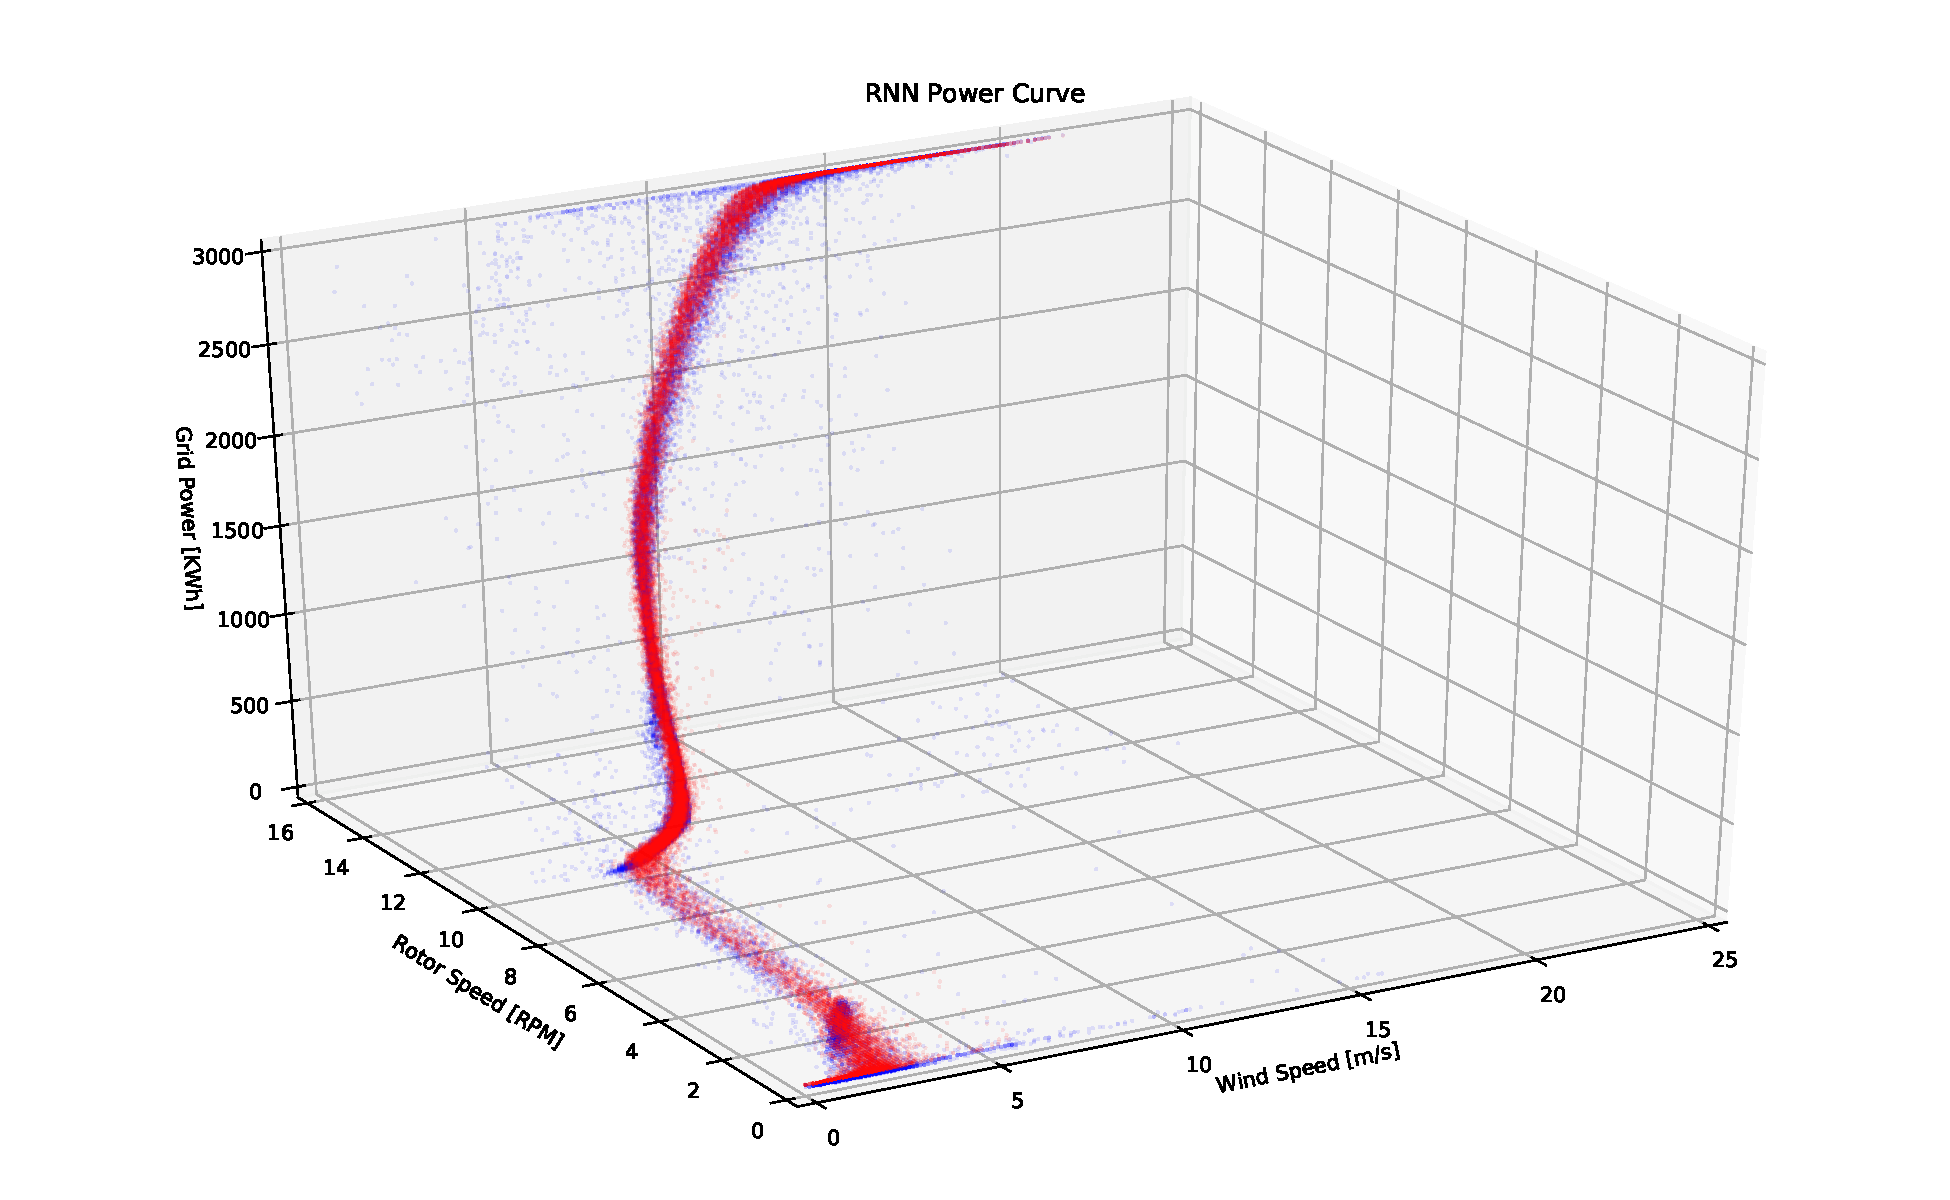
\includegraphics[width=0.47\textwidth]{rnn_power_curve_128_2_L1.pdf}
       \label{fig:2-rnn-power_curve-figb}
  }%
  \hfill
  \subfigure[LSTM with L1 loss]{
       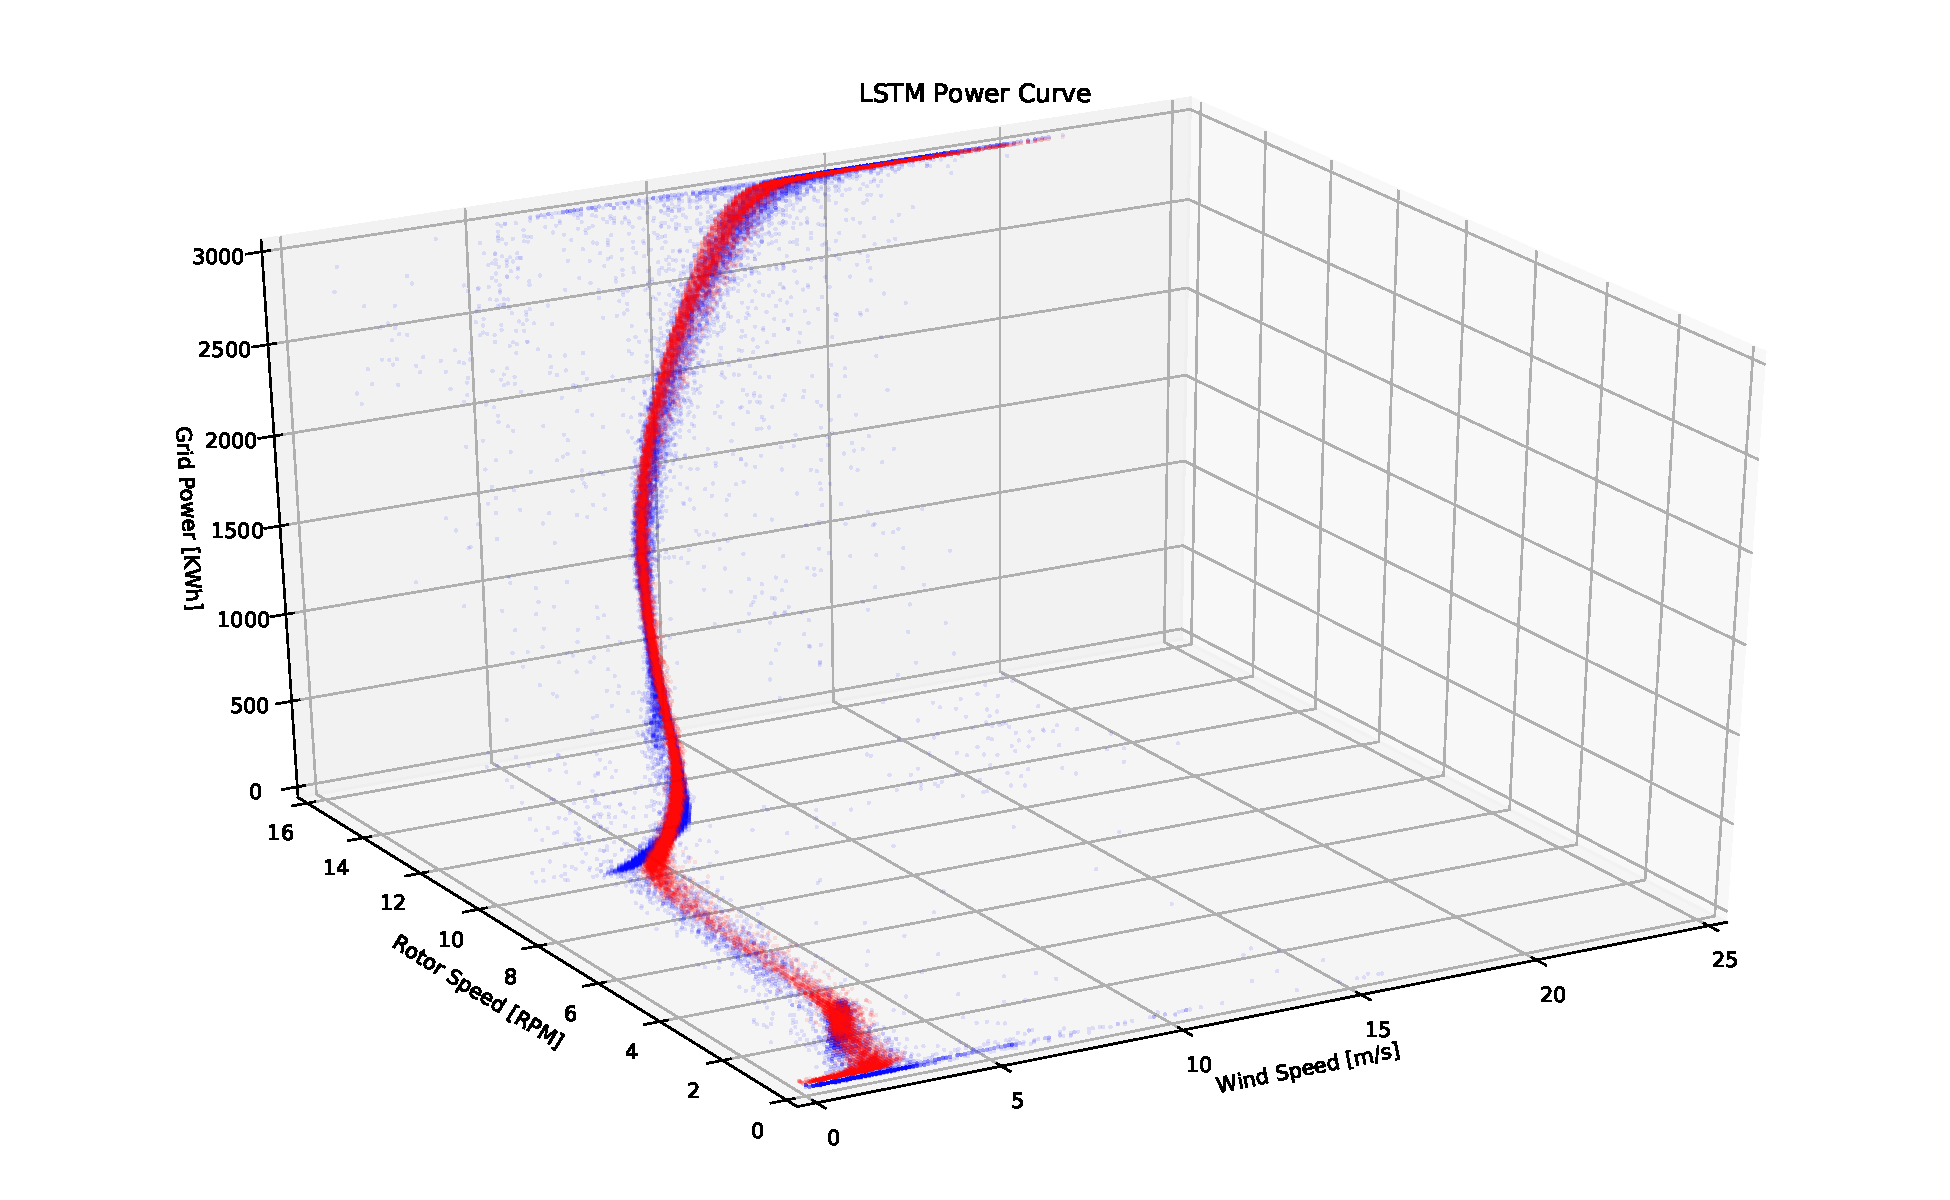
\includegraphics[width=0.47\textwidth]{lstm_power_curve_128_2_L1.pdf}
        \label{fig:2-lstm-power_curve-figb}
  }
  
  \subfigure[RNN with Tukey's biweight loss]{
       %\centering
       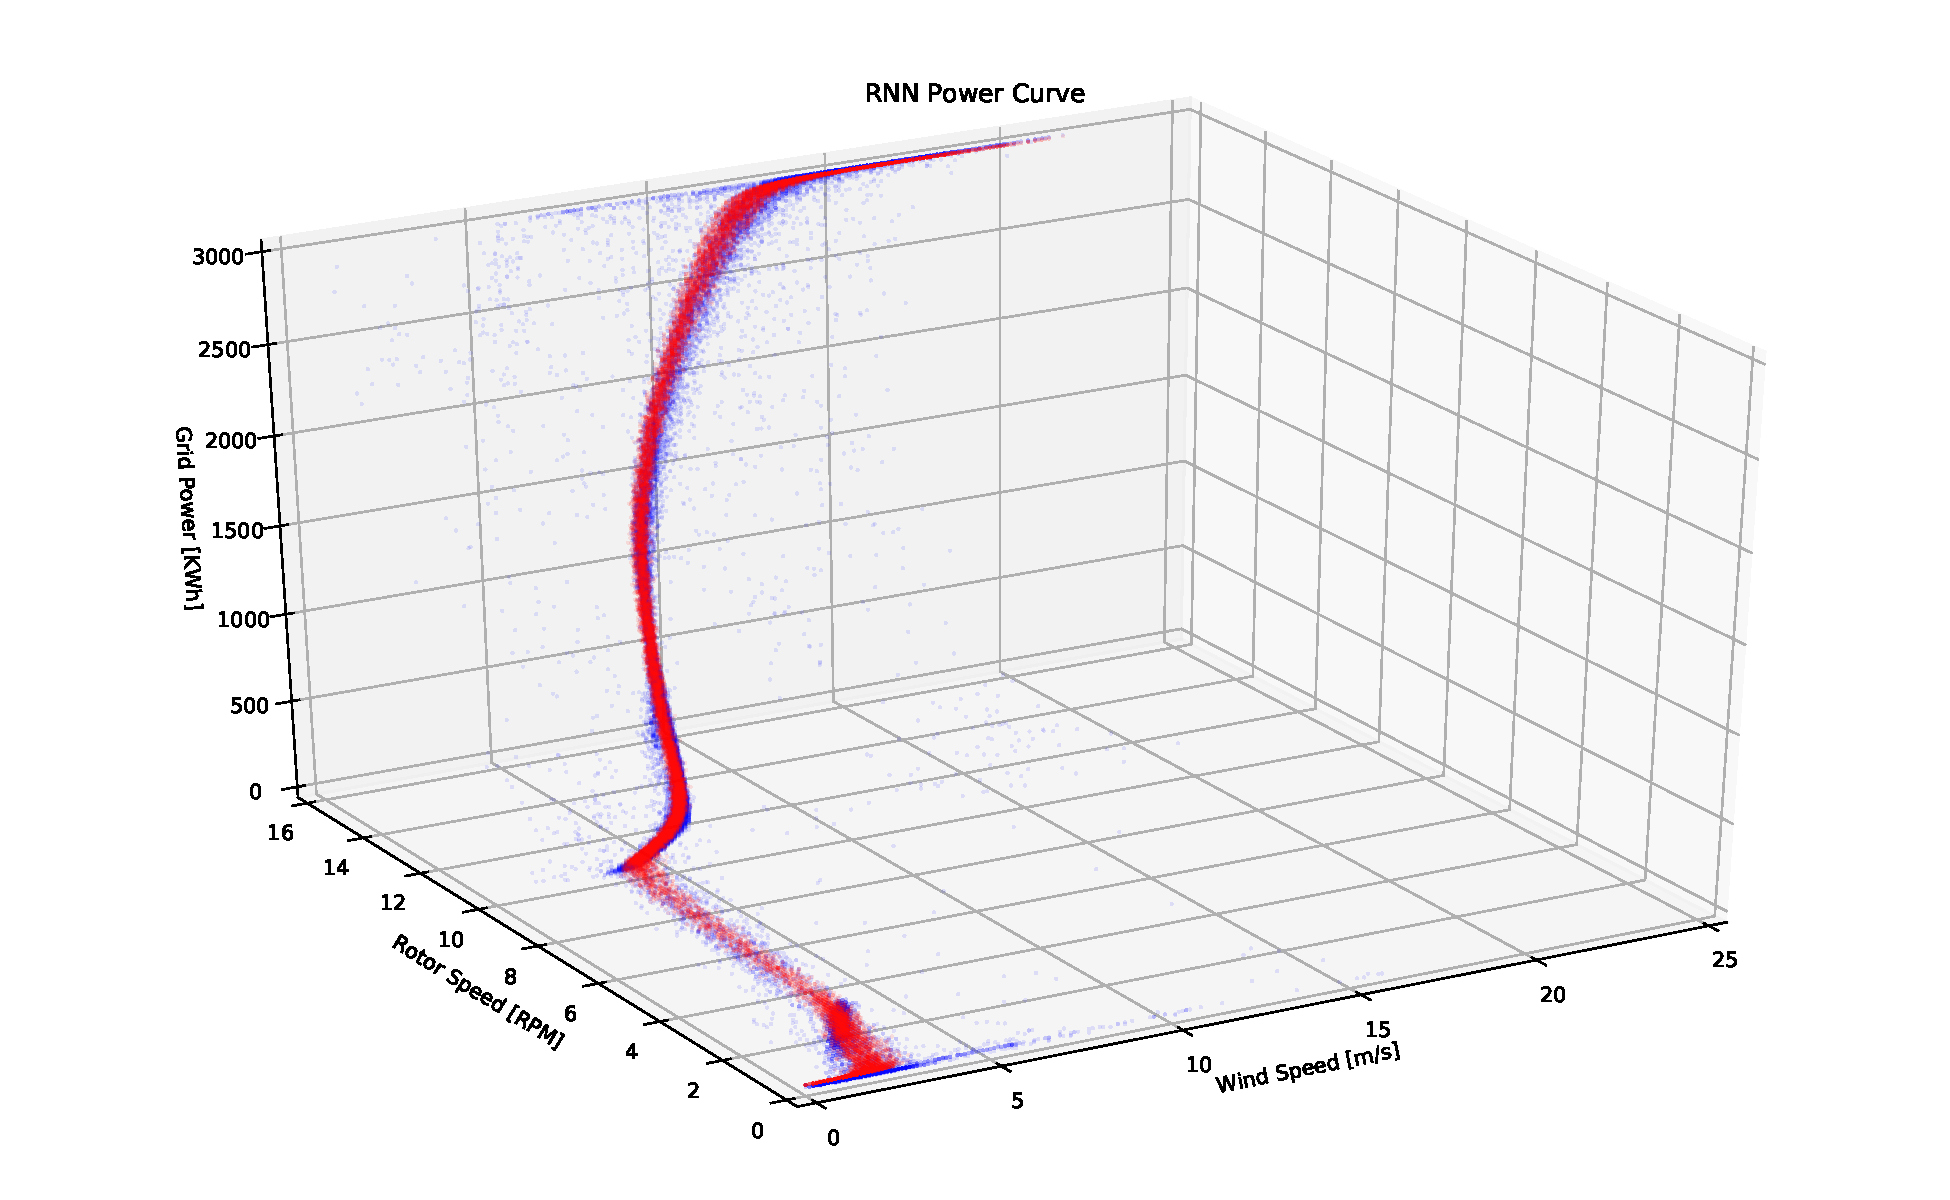
\includegraphics[width=0.47\textwidth]{rnn_power_curve_128_2_tukey.pdf}
        \label{fig:2-rnn-power_curve-figc}
  }%
  \hfill
  \subfigure[LSTM with Tukey's biweight loss]{
       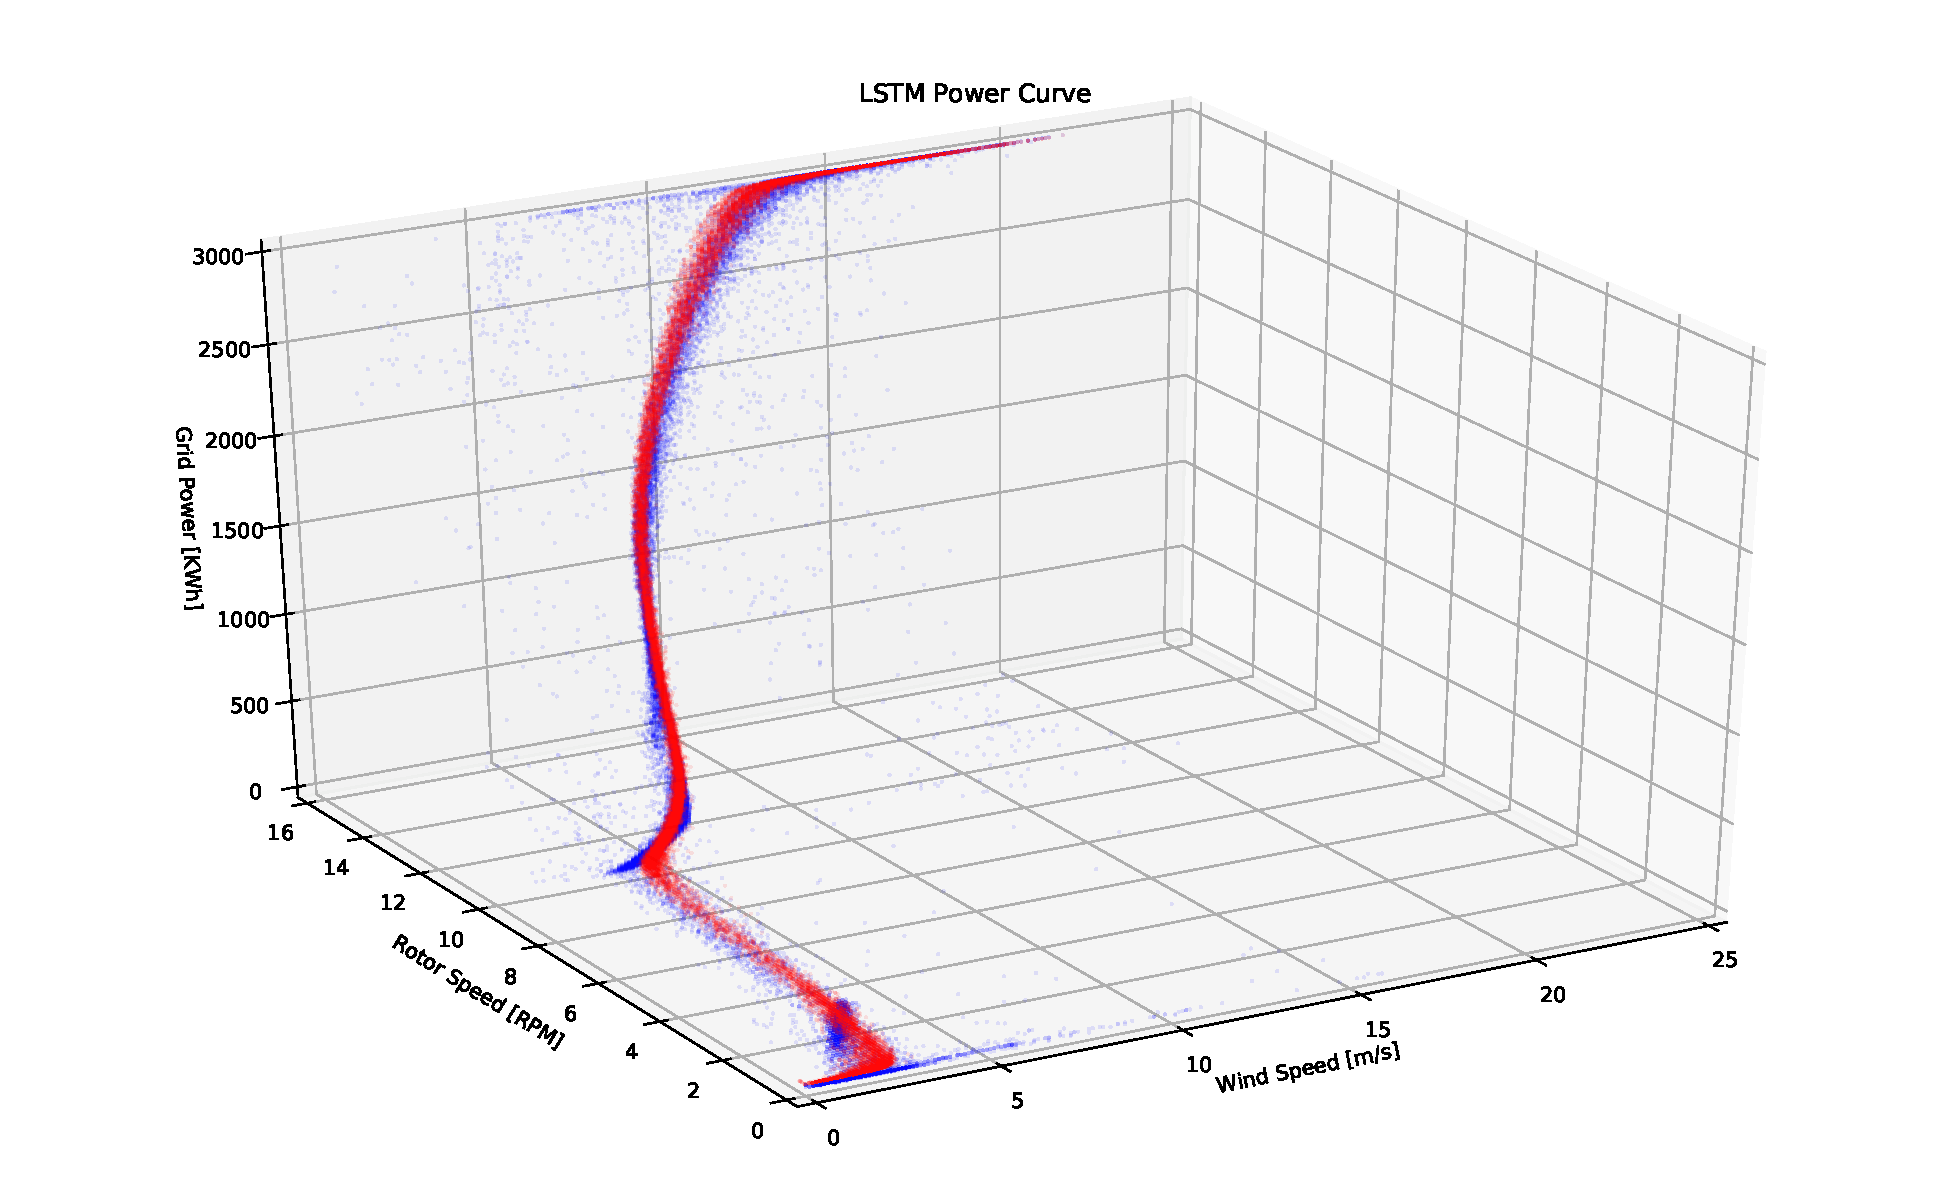
\includegraphics[width=0.47\textwidth]{lstm_power_curve_128_2_tukey.pdf}
       \label{fig:2-lstm-power_curve-figc}
  }
  \vspace{10pt}
  \caption{Generated from 2-layer network and observed power curves}
  \label{fig:2-deep_power_curves}
\end{figure}



\begin{figure}
    \centering
  \subfigure[RNN with MSE loss]{
       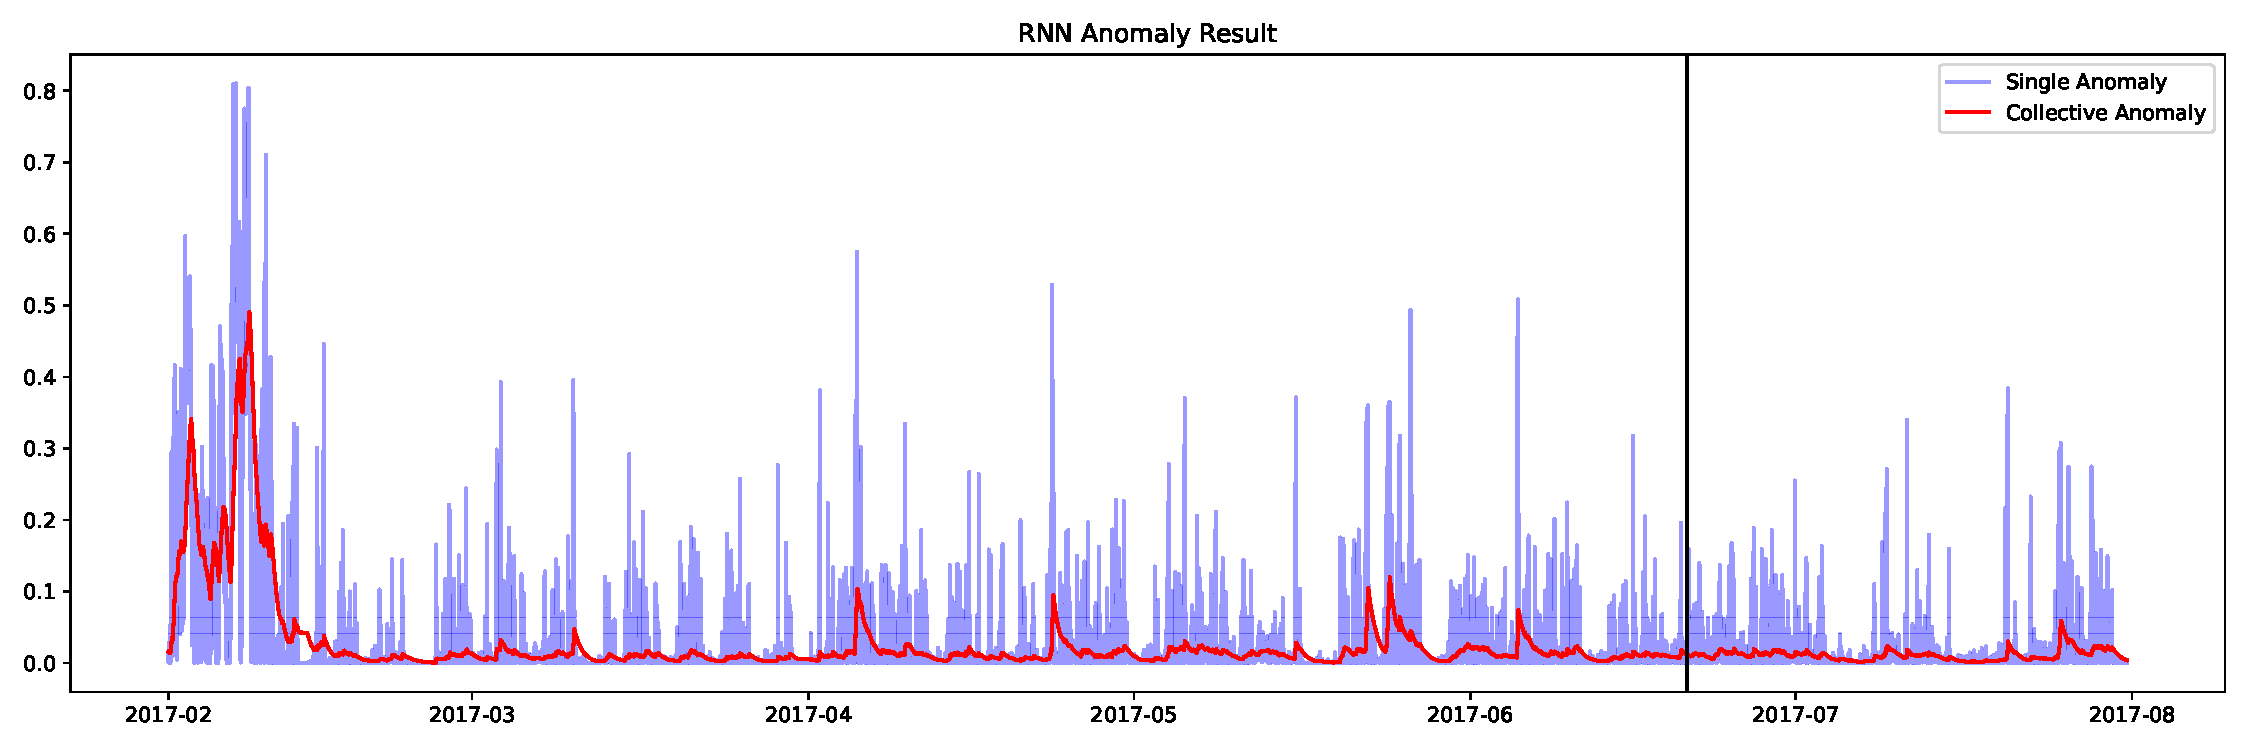
\includegraphics[width=0.48\textwidth]{rnn_anomaly_128_1_MSE.pdf}
       \label{fig:1-rnn-anomaly-figa}
    }%
  \hfill
  \subfigure[LSTM with MSE loss]{
       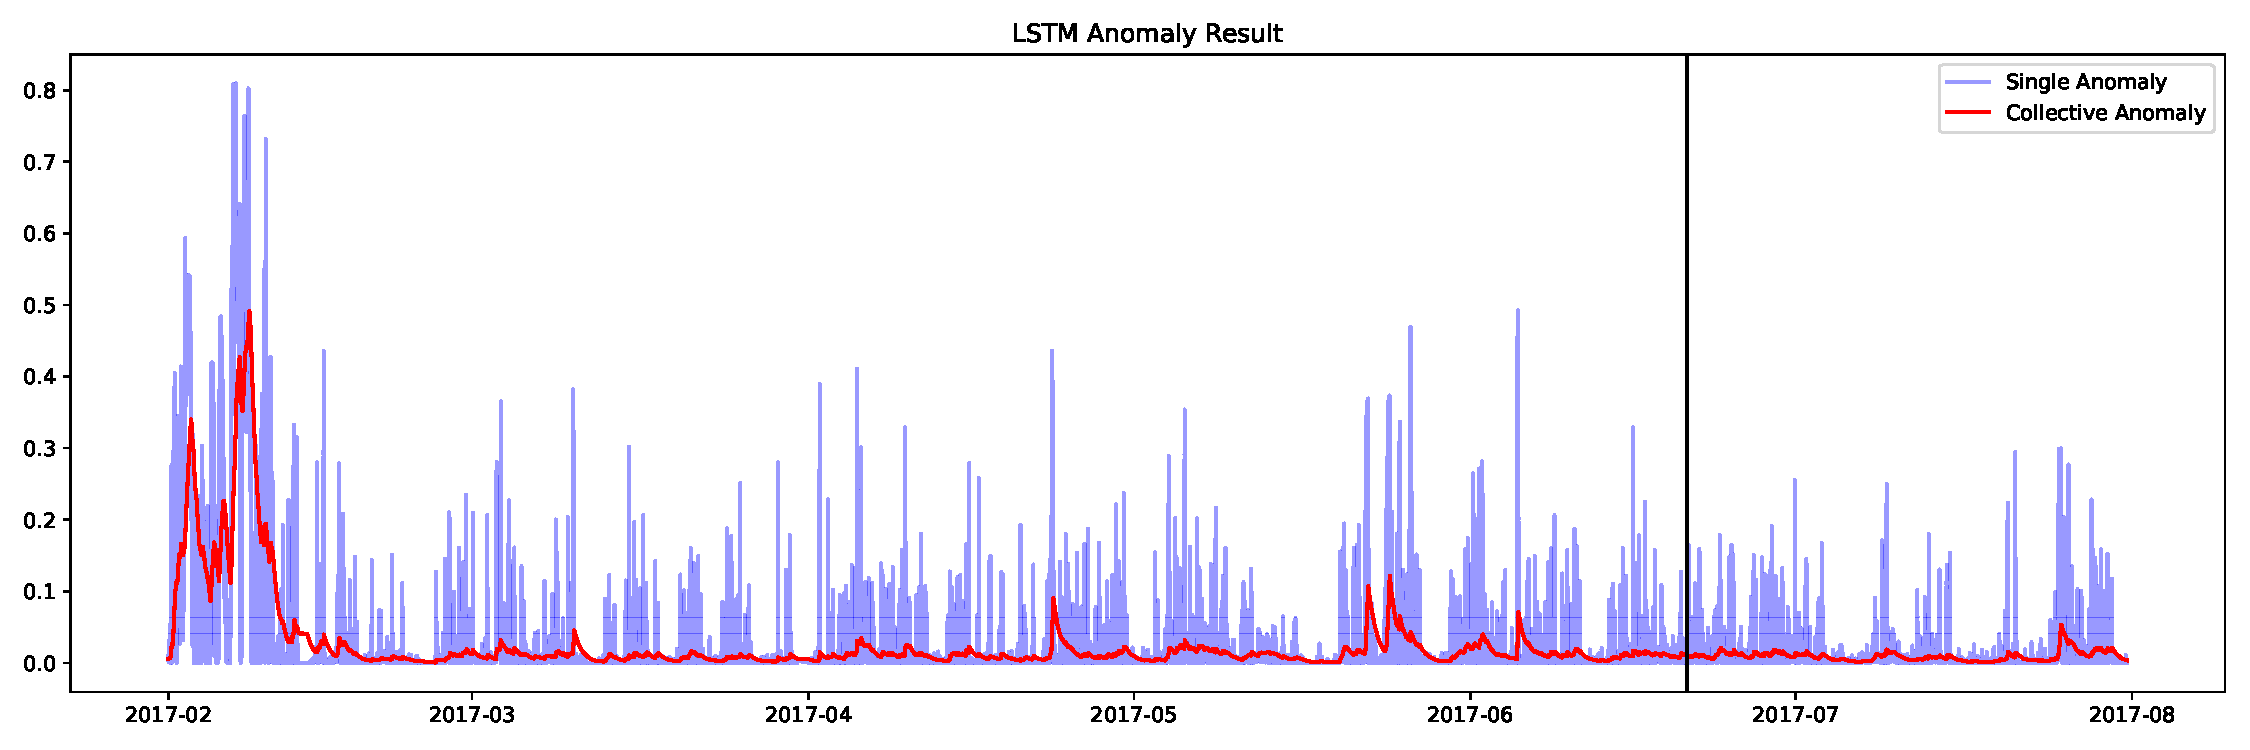
\includegraphics[width=0.48\textwidth]{lstm_anomaly_128_1_MSE.pdf}
       \label{fig:1-lstm-anomaly-figa}
  }
  
  \subfigure[RNN with L1 loss]{
       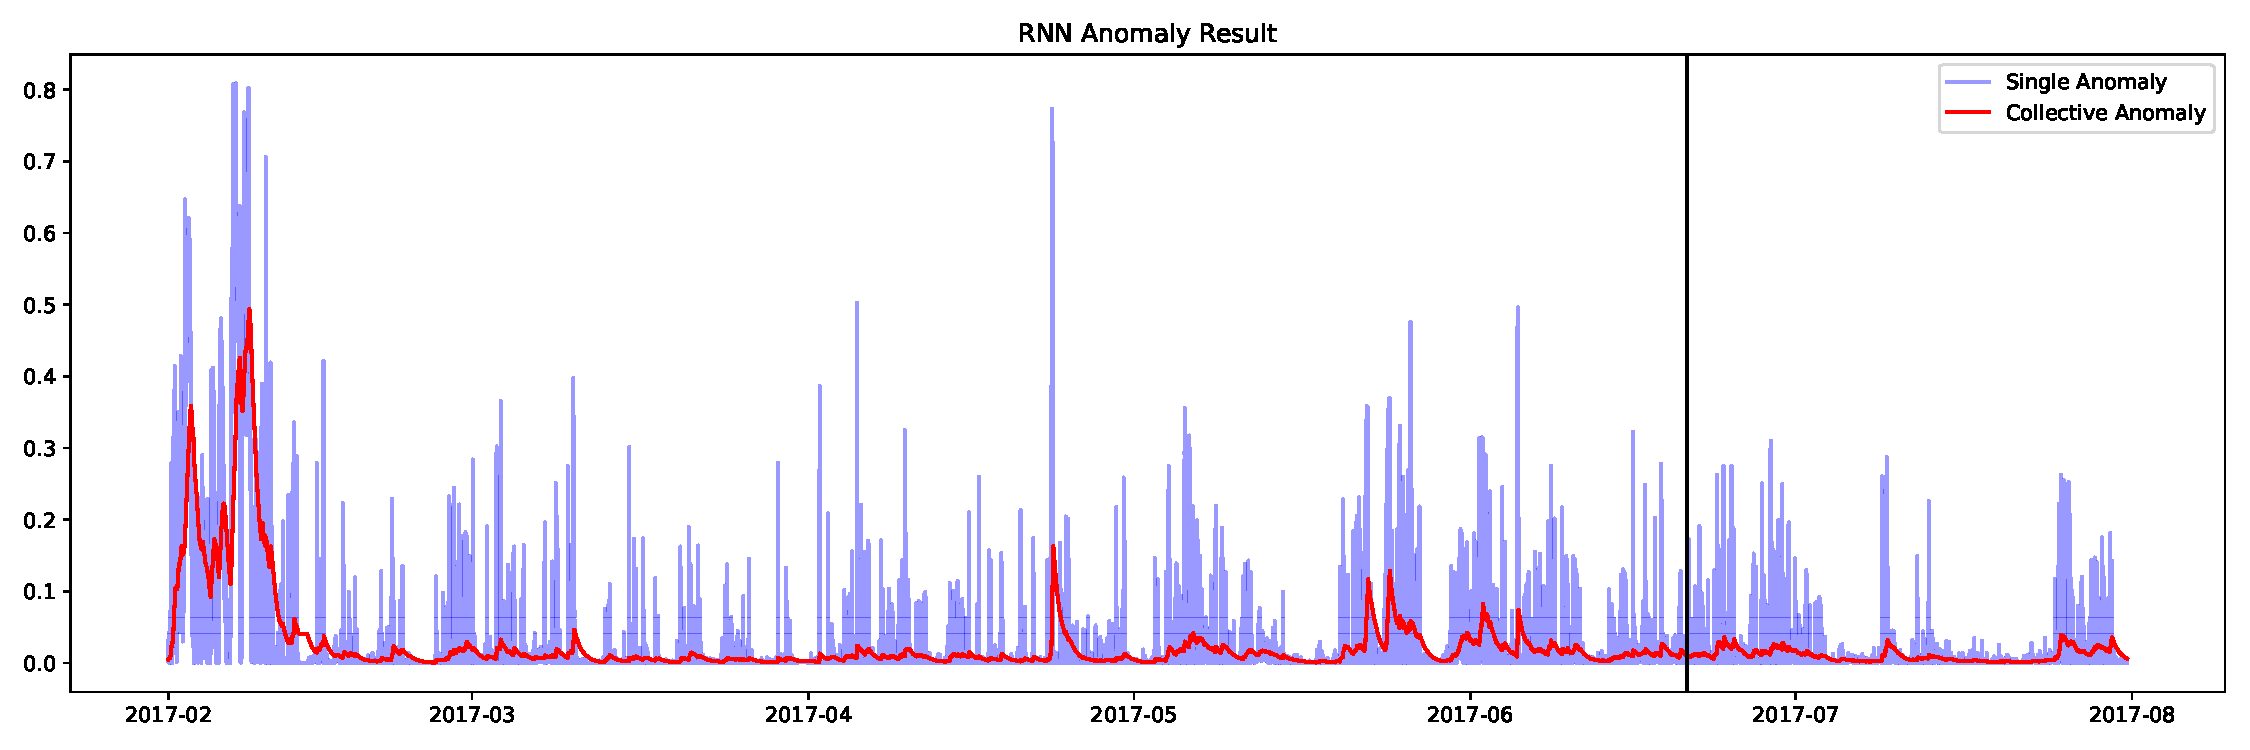
\includegraphics[width=0.48\textwidth]{rnn_anomaly_128_1_L1.pdf}
       \label{fig:1-rnn-anomaly-figb}
  }%
  \hfill
  \subfigure[LSTM with L1 loss]{
       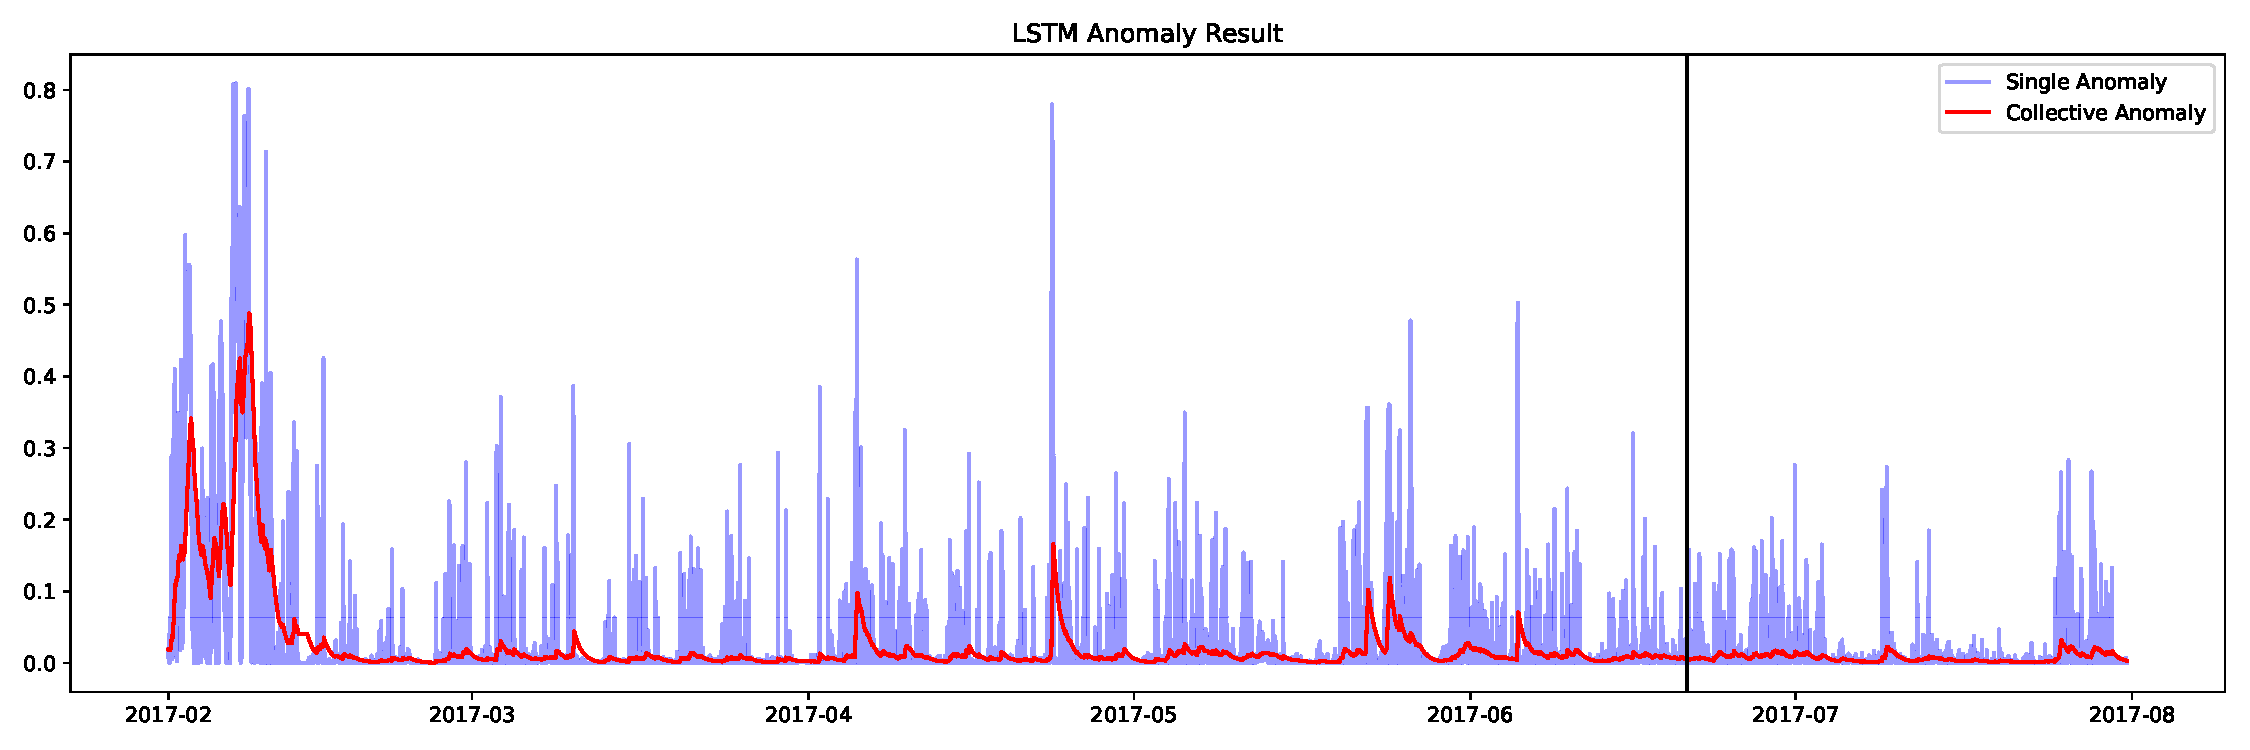
\includegraphics[width=0.48\textwidth]{lstm_anomaly_128_1_L1.pdf}
        \label{fig:1-lstm-anomaly-figb}
  }
  
  \subfigure[RNN with Tukey's biweight loss]{
       %\centering
       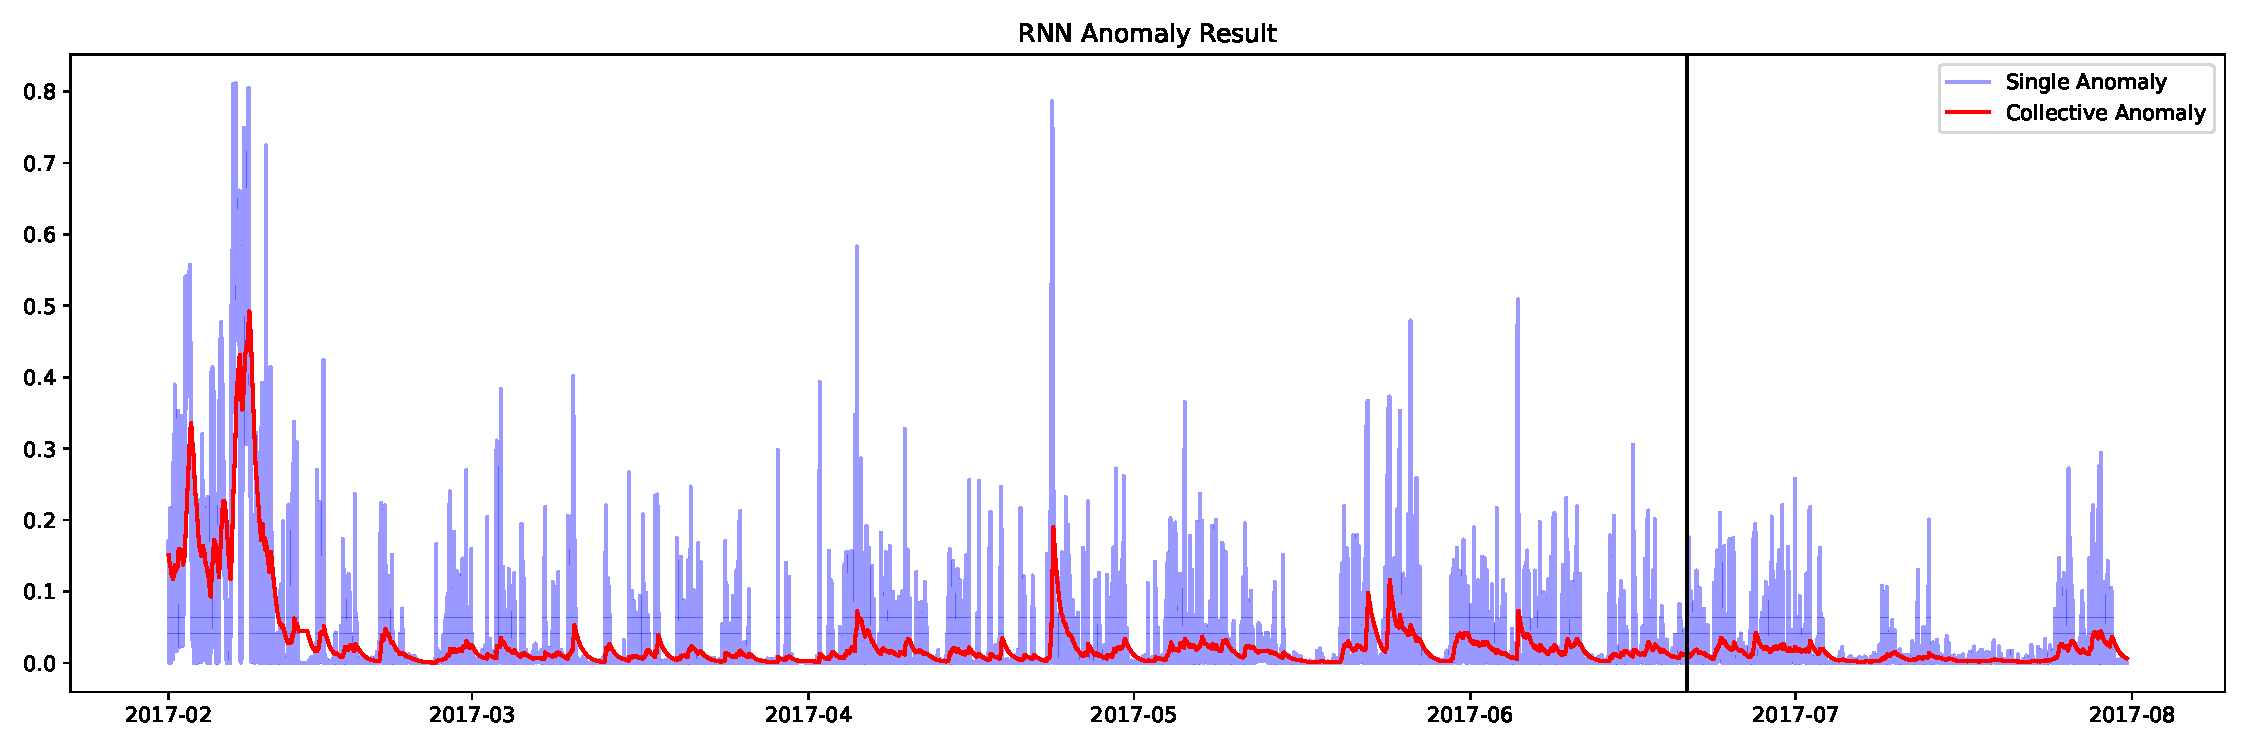
\includegraphics[width=0.48\textwidth]{rnn_anomaly_128_1_tukey.pdf}
        \label{fig:1-rnn-anomaly-figc}
  }%
  \hfill
  \subfigure[LSTM with Tukey's biweight loss]{
       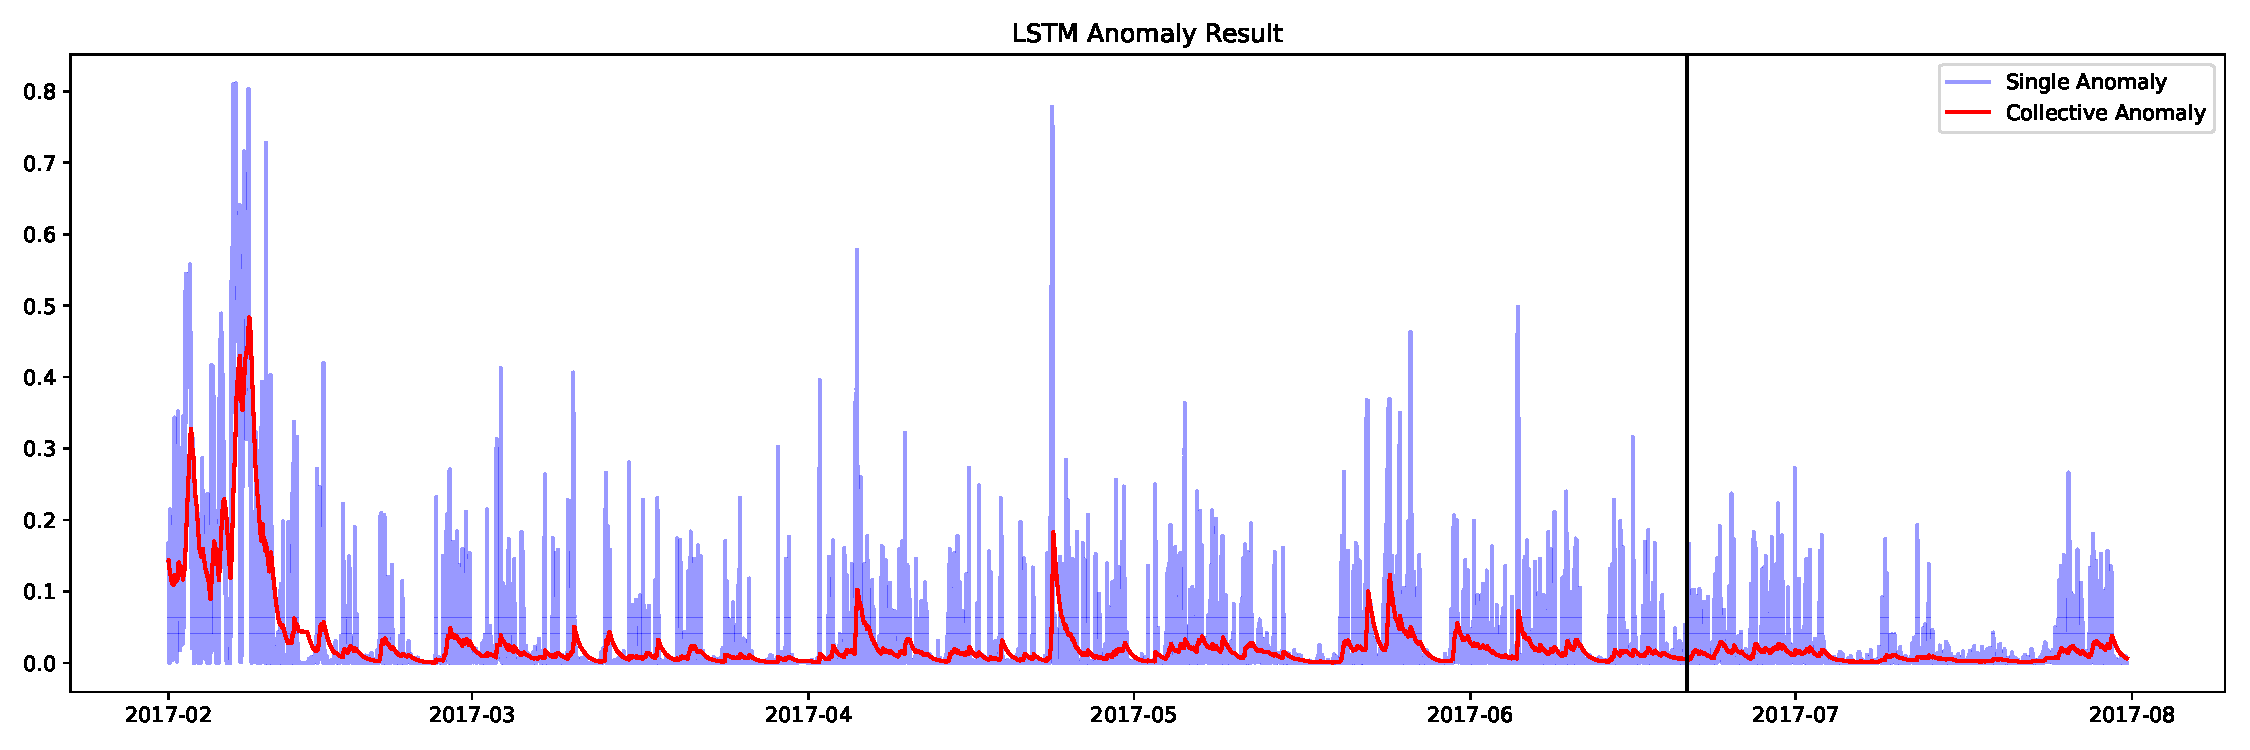
\includegraphics[width=0.48\textwidth]{lstm_anomaly_128_1_tukey.pdf}
       \label{fig:1-lstm-anomaly-figc}
  }
  \vspace{10pt}
  \caption{Anomaly scores of the $1$-layered networks on test data.}
  \label{fig:1-deep_anomalies}
\end{figure}


\begin{figure}
    \centering
  \subfigure[RNN with MSE loss]{
       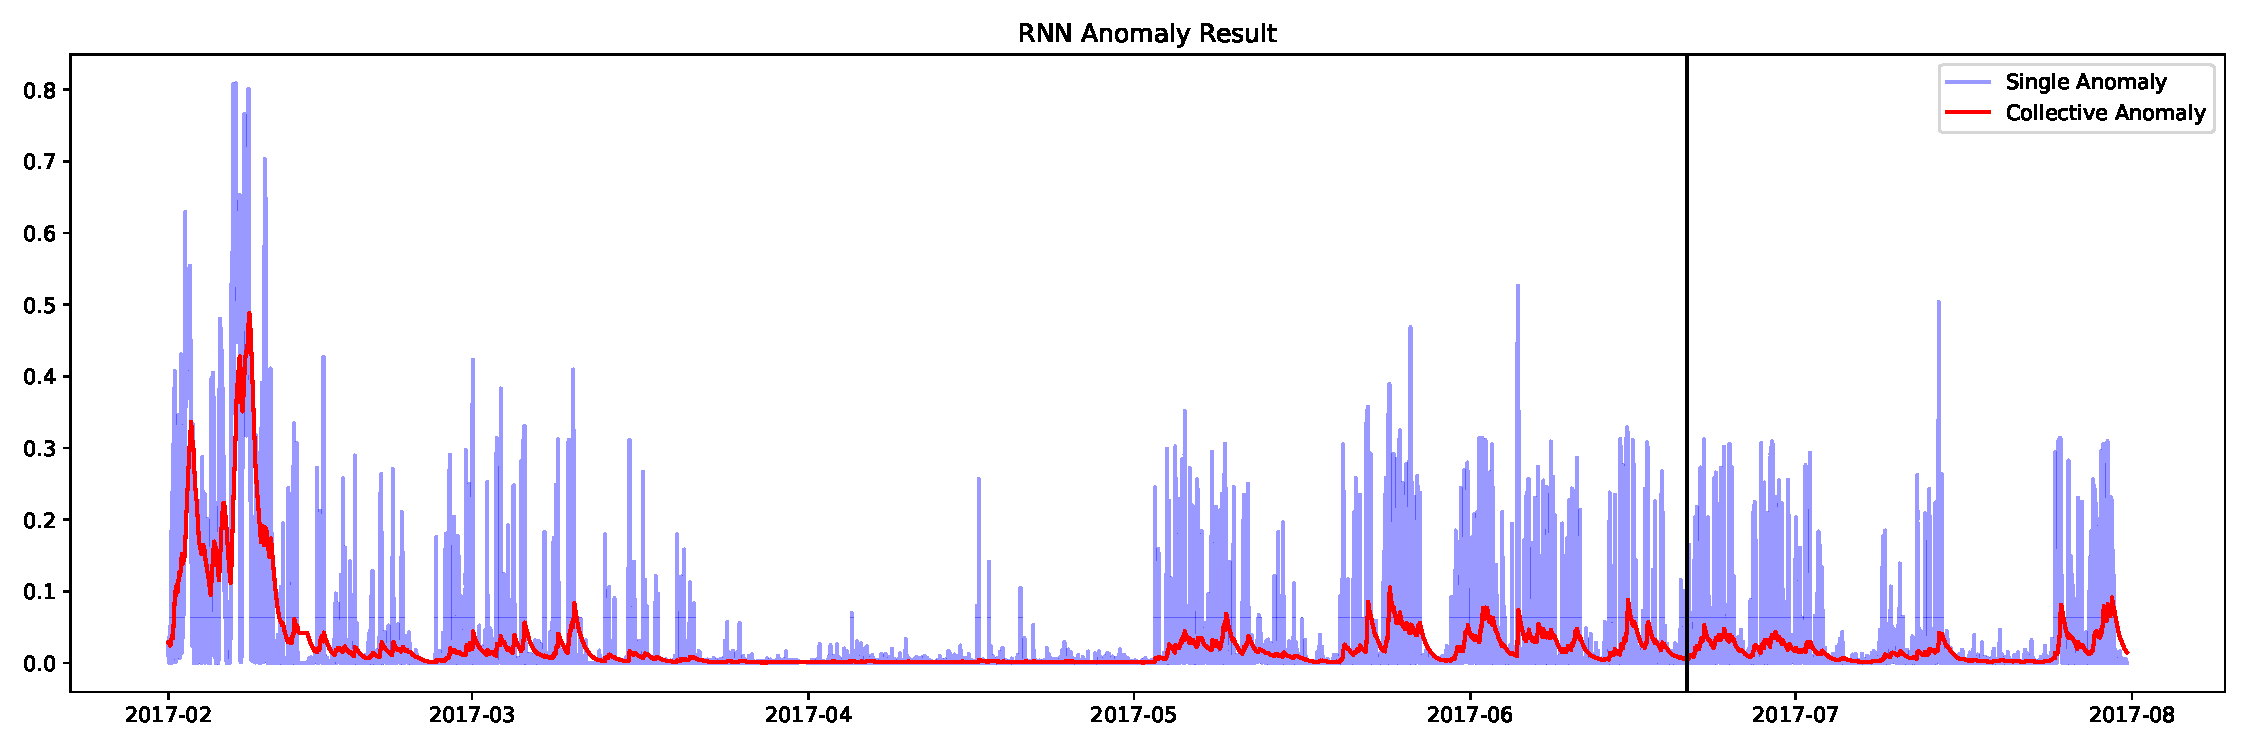
\includegraphics[width=0.48\textwidth]{rnn_anomaly_128_2_MSE.pdf}
       \label{fig:2-rnn-anomaly-figa}
    }%
  \hfill
  \subfigure[LSTM with MSE loss]{
       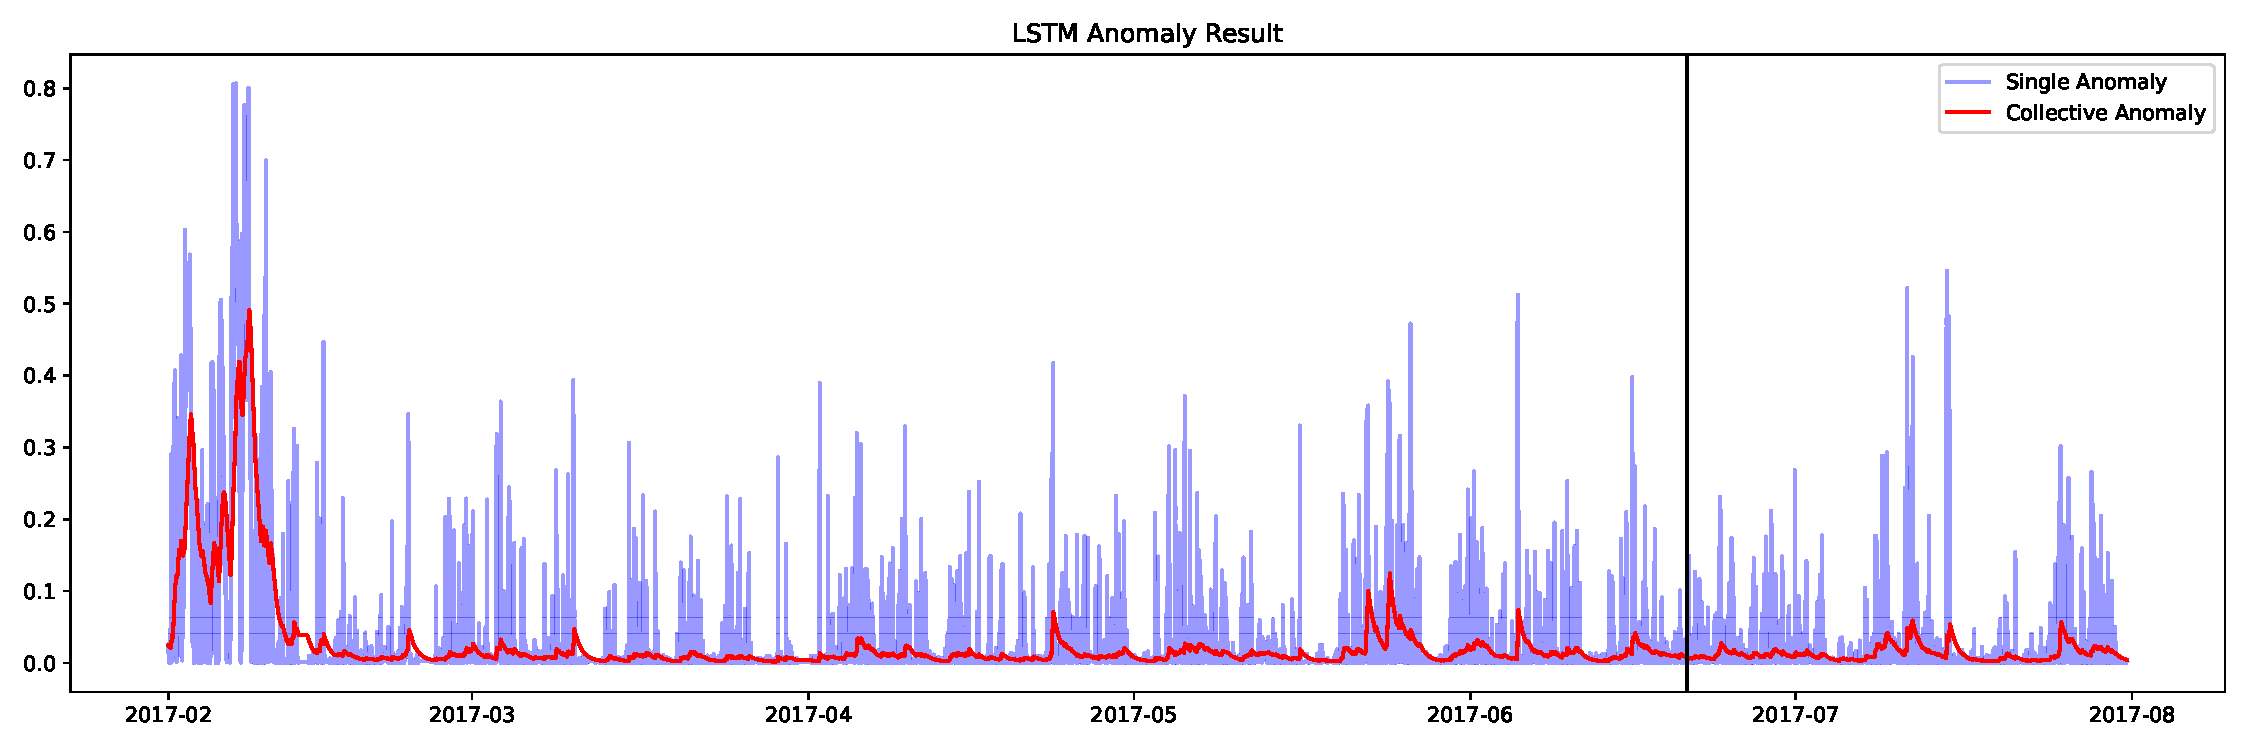
\includegraphics[width=0.48\textwidth]{lstm_anomaly_128_2_MSE.pdf}
       \label{fig:2-lstm-anomaly-figa}
  }
  
  \subfigure[RNN with L1 loss]{
       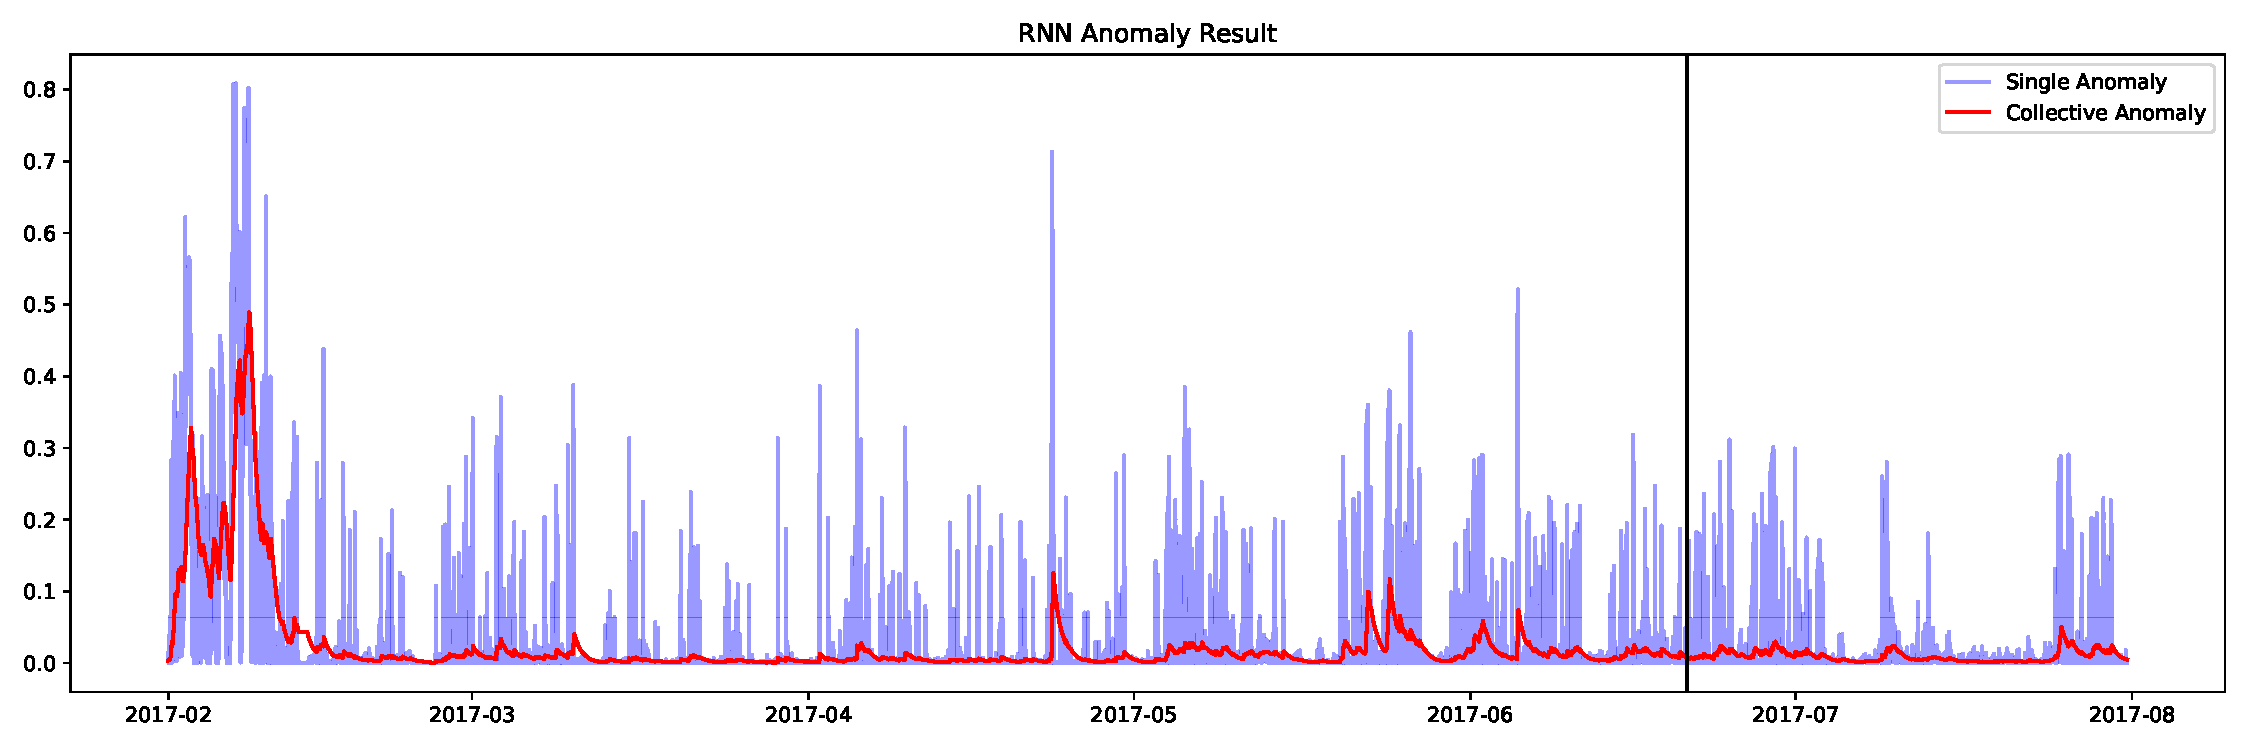
\includegraphics[width=0.48\textwidth]{rnn_anomaly_128_2_L1.pdf}
       \label{fig:2-rnn-anomaly-figb}
  }%
  \hfill
  \subfigure[LSTM with L1 loss]{
       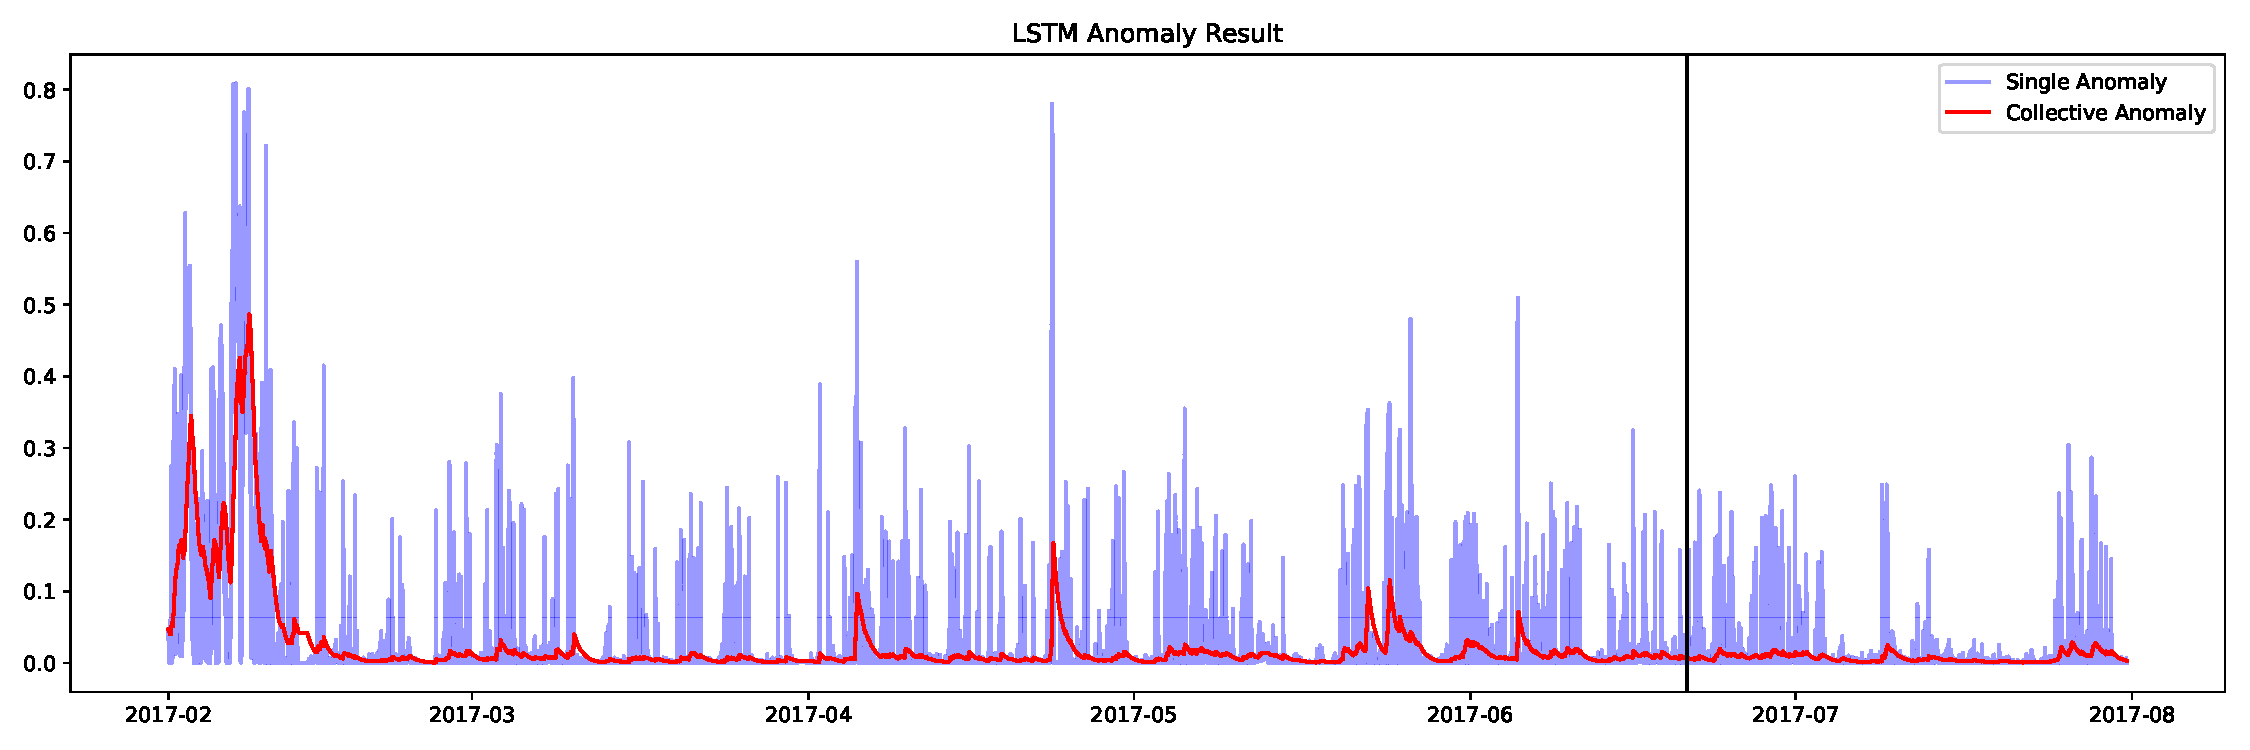
\includegraphics[width=0.48\textwidth]{lstm_anomaly_128_2_L1.pdf}
        \label{fig:2-lstm-anomaly-figb}
  }
  
  \subfigure[RNN with Tukey's biweight loss]{
       %\centering
       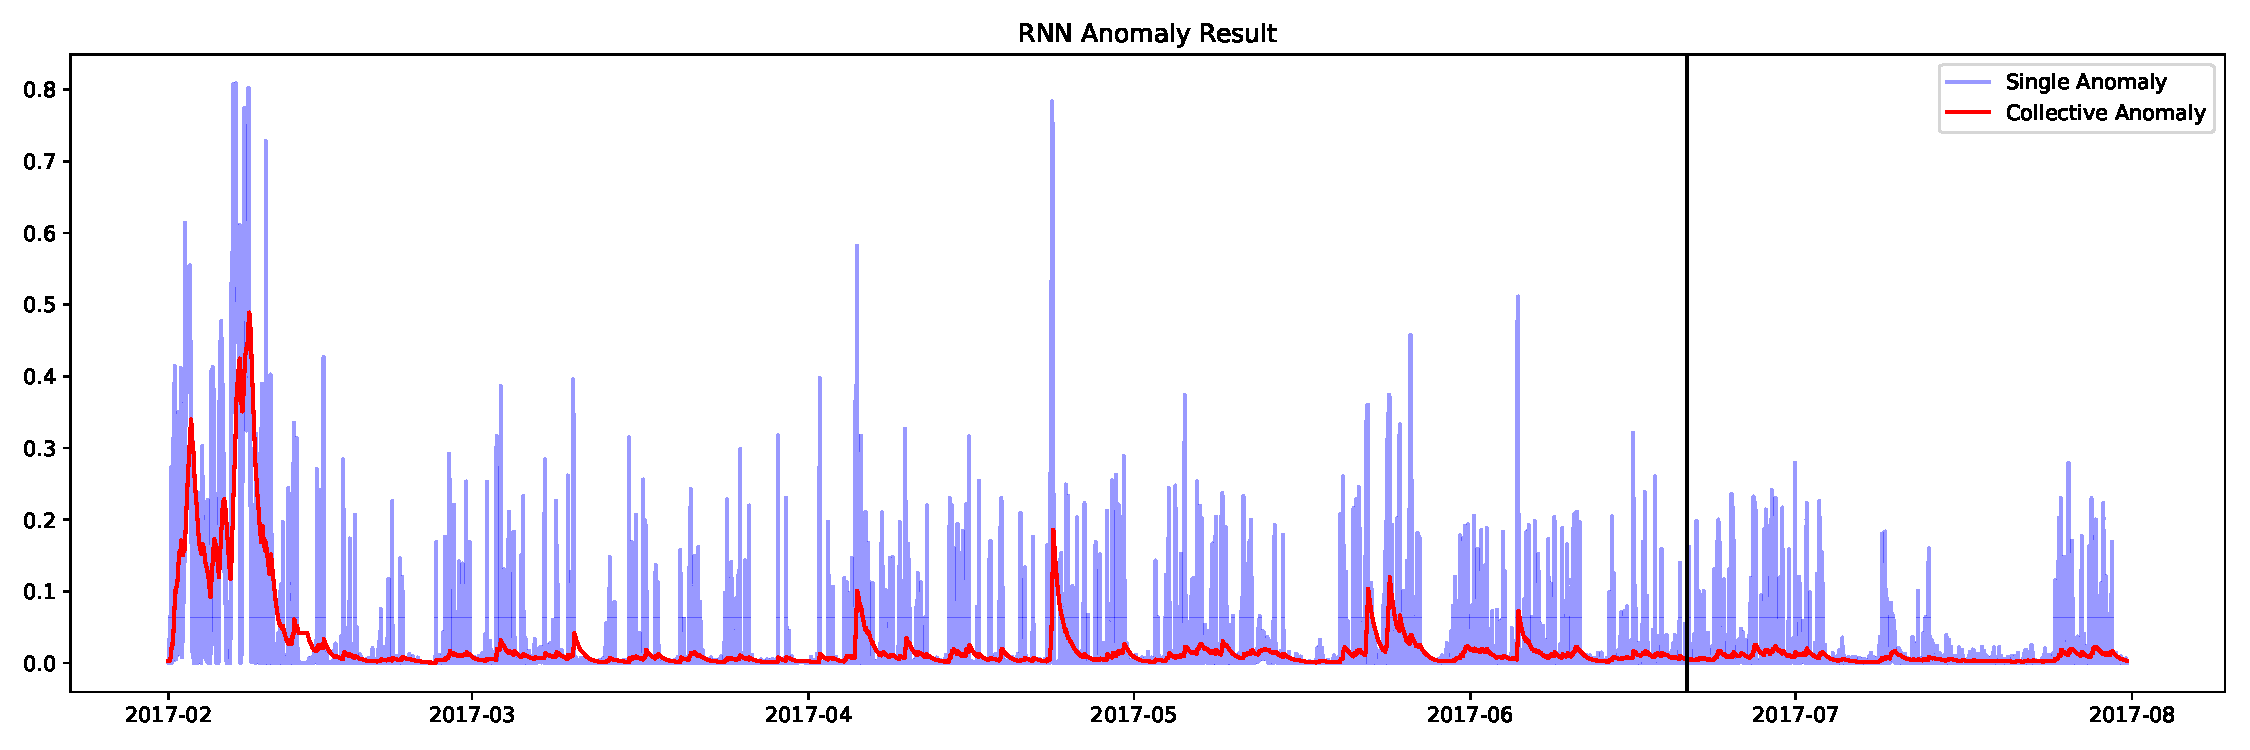
\includegraphics[width=0.48\textwidth]{rnn_anomaly_128_2_tukey.pdf}
        \label{fig:2-rnn-anomaly-figc}
  }%
  \hfill
  \subfigure[LSTM with Tukey's biweight loss]{
       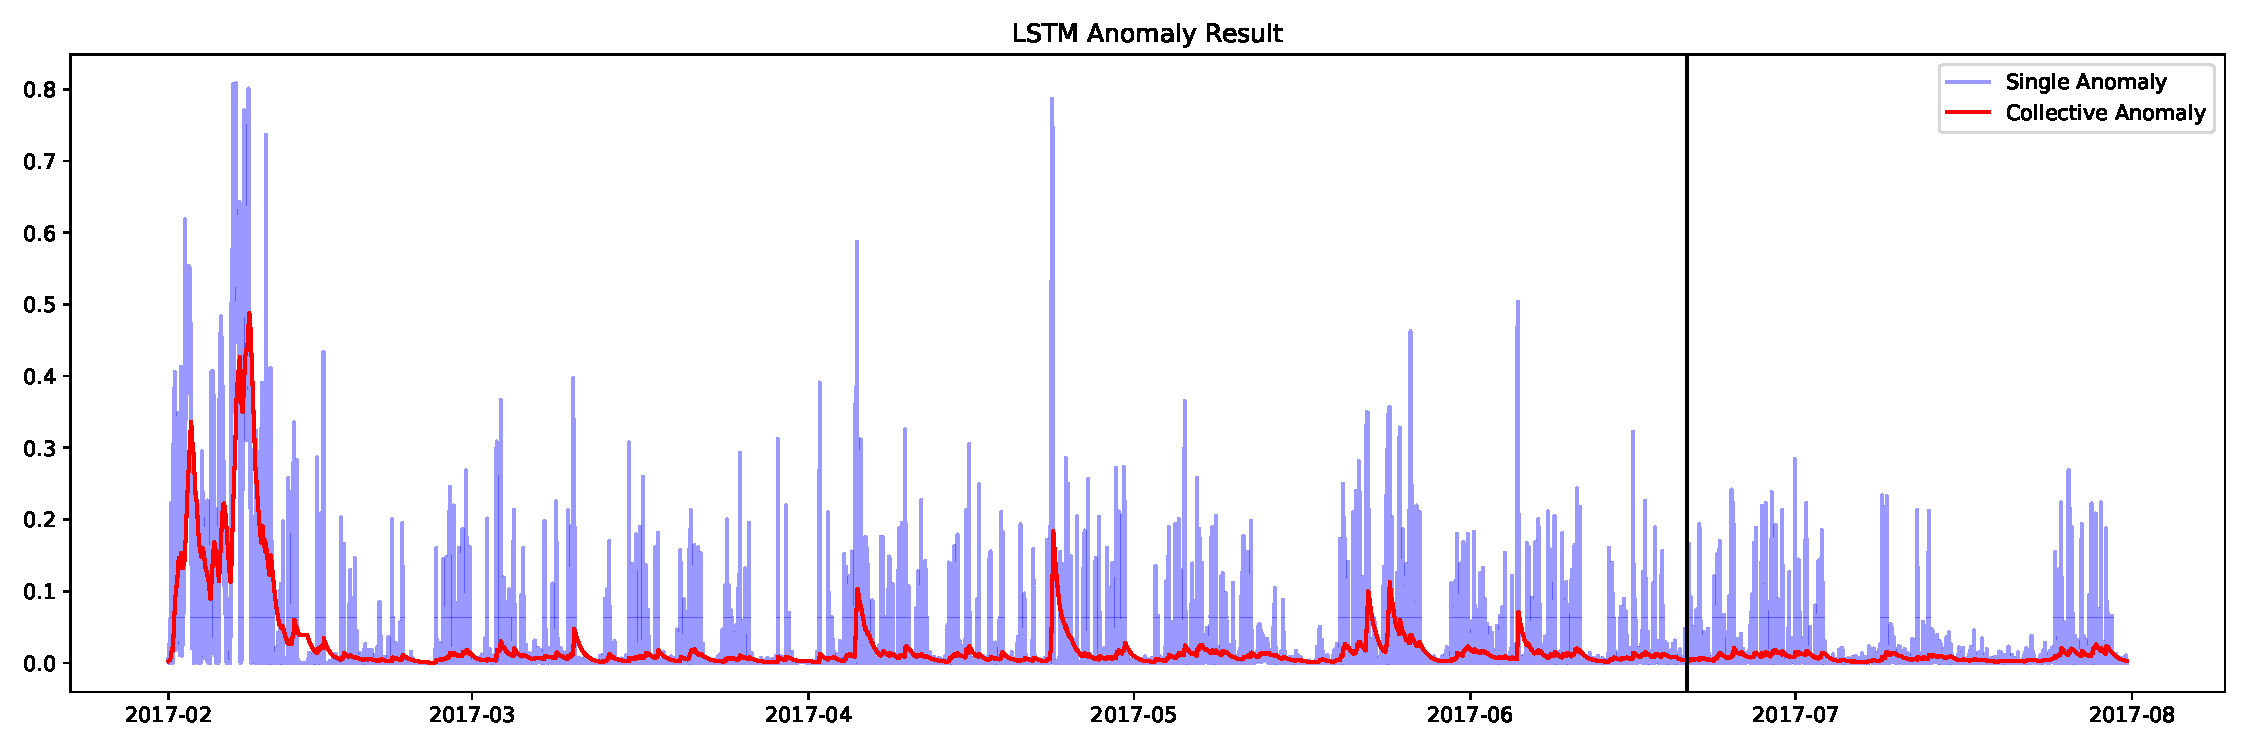
\includegraphics[width=0.48\textwidth]{lstm_anomaly_128_2_tukey.pdf}
       \label{fig:2-lstm-anomaly-figc}
  }
  \vspace{10pt}
  \caption{Anomaly scores of the $2$-layered (stacked) networks on test data.}
  \label{fig:2-deep_anomalies}
\end{figure}